% Options for packages loaded elsewhere
\PassOptionsToPackage{unicode}{hyperref}
\PassOptionsToPackage{hyphens}{url}
%
\documentclass[
]{article}
\usepackage{amsmath,amssymb}
\usepackage{lmodern}
\usepackage{iftex}
\ifPDFTeX
  \usepackage[T1]{fontenc}
  \usepackage[utf8]{inputenc}
  \usepackage{textcomp} % provide euro and other symbols
\else % if luatex or xetex
  \usepackage{unicode-math}
  \defaultfontfeatures{Scale=MatchLowercase}
  \defaultfontfeatures[\rmfamily]{Ligatures=TeX,Scale=1}
\fi
% Use upquote if available, for straight quotes in verbatim environments
\IfFileExists{upquote.sty}{\usepackage{upquote}}{}
\IfFileExists{microtype.sty}{% use microtype if available
  \usepackage[]{microtype}
  \UseMicrotypeSet[protrusion]{basicmath} % disable protrusion for tt fonts
}{}
\makeatletter
\@ifundefined{KOMAClassName}{% if non-KOMA class
  \IfFileExists{parskip.sty}{%
    \usepackage{parskip}
  }{% else
    \setlength{\parindent}{0pt}
    \setlength{\parskip}{6pt plus 2pt minus 1pt}}
}{% if KOMA class
  \KOMAoptions{parskip=half}}
\makeatother
\usepackage{xcolor}
\usepackage[margin=1in]{geometry}
\usepackage{color}
\usepackage{fancyvrb}
\newcommand{\VerbBar}{|}
\newcommand{\VERB}{\Verb[commandchars=\\\{\}]}
\DefineVerbatimEnvironment{Highlighting}{Verbatim}{commandchars=\\\{\}}
% Add ',fontsize=\small' for more characters per line
\usepackage{framed}
\definecolor{shadecolor}{RGB}{248,248,248}
\newenvironment{Shaded}{\begin{snugshade}}{\end{snugshade}}
\newcommand{\AlertTok}[1]{\textcolor[rgb]{0.94,0.16,0.16}{#1}}
\newcommand{\AnnotationTok}[1]{\textcolor[rgb]{0.56,0.35,0.01}{\textbf{\textit{#1}}}}
\newcommand{\AttributeTok}[1]{\textcolor[rgb]{0.77,0.63,0.00}{#1}}
\newcommand{\BaseNTok}[1]{\textcolor[rgb]{0.00,0.00,0.81}{#1}}
\newcommand{\BuiltInTok}[1]{#1}
\newcommand{\CharTok}[1]{\textcolor[rgb]{0.31,0.60,0.02}{#1}}
\newcommand{\CommentTok}[1]{\textcolor[rgb]{0.56,0.35,0.01}{\textit{#1}}}
\newcommand{\CommentVarTok}[1]{\textcolor[rgb]{0.56,0.35,0.01}{\textbf{\textit{#1}}}}
\newcommand{\ConstantTok}[1]{\textcolor[rgb]{0.00,0.00,0.00}{#1}}
\newcommand{\ControlFlowTok}[1]{\textcolor[rgb]{0.13,0.29,0.53}{\textbf{#1}}}
\newcommand{\DataTypeTok}[1]{\textcolor[rgb]{0.13,0.29,0.53}{#1}}
\newcommand{\DecValTok}[1]{\textcolor[rgb]{0.00,0.00,0.81}{#1}}
\newcommand{\DocumentationTok}[1]{\textcolor[rgb]{0.56,0.35,0.01}{\textbf{\textit{#1}}}}
\newcommand{\ErrorTok}[1]{\textcolor[rgb]{0.64,0.00,0.00}{\textbf{#1}}}
\newcommand{\ExtensionTok}[1]{#1}
\newcommand{\FloatTok}[1]{\textcolor[rgb]{0.00,0.00,0.81}{#1}}
\newcommand{\FunctionTok}[1]{\textcolor[rgb]{0.00,0.00,0.00}{#1}}
\newcommand{\ImportTok}[1]{#1}
\newcommand{\InformationTok}[1]{\textcolor[rgb]{0.56,0.35,0.01}{\textbf{\textit{#1}}}}
\newcommand{\KeywordTok}[1]{\textcolor[rgb]{0.13,0.29,0.53}{\textbf{#1}}}
\newcommand{\NormalTok}[1]{#1}
\newcommand{\OperatorTok}[1]{\textcolor[rgb]{0.81,0.36,0.00}{\textbf{#1}}}
\newcommand{\OtherTok}[1]{\textcolor[rgb]{0.56,0.35,0.01}{#1}}
\newcommand{\PreprocessorTok}[1]{\textcolor[rgb]{0.56,0.35,0.01}{\textit{#1}}}
\newcommand{\RegionMarkerTok}[1]{#1}
\newcommand{\SpecialCharTok}[1]{\textcolor[rgb]{0.00,0.00,0.00}{#1}}
\newcommand{\SpecialStringTok}[1]{\textcolor[rgb]{0.31,0.60,0.02}{#1}}
\newcommand{\StringTok}[1]{\textcolor[rgb]{0.31,0.60,0.02}{#1}}
\newcommand{\VariableTok}[1]{\textcolor[rgb]{0.00,0.00,0.00}{#1}}
\newcommand{\VerbatimStringTok}[1]{\textcolor[rgb]{0.31,0.60,0.02}{#1}}
\newcommand{\WarningTok}[1]{\textcolor[rgb]{0.56,0.35,0.01}{\textbf{\textit{#1}}}}
\usepackage{longtable,booktabs,array}
\usepackage{calc} % for calculating minipage widths
% Correct order of tables after \paragraph or \subparagraph
\usepackage{etoolbox}
\makeatletter
\patchcmd\longtable{\par}{\if@noskipsec\mbox{}\fi\par}{}{}
\makeatother
% Allow footnotes in longtable head/foot
\IfFileExists{footnotehyper.sty}{\usepackage{footnotehyper}}{\usepackage{footnote}}
\makesavenoteenv{longtable}
\usepackage{graphicx}
\makeatletter
\def\maxwidth{\ifdim\Gin@nat@width>\linewidth\linewidth\else\Gin@nat@width\fi}
\def\maxheight{\ifdim\Gin@nat@height>\textheight\textheight\else\Gin@nat@height\fi}
\makeatother
% Scale images if necessary, so that they will not overflow the page
% margins by default, and it is still possible to overwrite the defaults
% using explicit options in \includegraphics[width, height, ...]{}
\setkeys{Gin}{width=\maxwidth,height=\maxheight,keepaspectratio}
% Set default figure placement to htbp
\makeatletter
\def\fps@figure{htbp}
\makeatother
\setlength{\emergencystretch}{3em} % prevent overfull lines
\providecommand{\tightlist}{%
  \setlength{\itemsep}{0pt}\setlength{\parskip}{0pt}}
\setcounter{secnumdepth}{5}
\ifLuaTeX
  \usepackage{selnolig}  % disable illegal ligatures
\fi
\IfFileExists{bookmark.sty}{\usepackage{bookmark}}{\usepackage{hyperref}}
\IfFileExists{xurl.sty}{\usepackage{xurl}}{} % add URL line breaks if available
\urlstyle{same} % disable monospaced font for URLs
\hypersetup{
  pdftitle={Burrows Bay Octopus Phylogeny},
  pdfauthor={Kirt Onthank},
  hidelinks,
  pdfcreator={LaTeX via pandoc}}

\title{Burrows Bay Octopus Phylogeny}
\author{Kirt Onthank}
\date{2022-09-25}

\begin{document}
\maketitle

{
\setcounter{tocdepth}{3}
\tableofcontents
}
\hypertarget{loading-libraries}{%
\section{Loading Libraries}\label{loading-libraries}}

\begin{Shaded}
\begin{Highlighting}[]
\FunctionTok{library}\NormalTok{(ape)}
\FunctionTok{library}\NormalTok{(xlsx)}
\FunctionTok{library}\NormalTok{(insect)}
\FunctionTok{library}\NormalTok{(aphid)}
\FunctionTok{library}\NormalTok{(DECIPHER)}
\FunctionTok{library}\NormalTok{(magrittr)}
\FunctionTok{library}\NormalTok{(phangorn)}
\FunctionTok{library}\NormalTok{(rwty)}
\FunctionTok{library}\NormalTok{(stringi)}
\FunctionTok{library}\NormalTok{(Biostrings)}
\FunctionTok{library}\NormalTok{(dplyr)}
\FunctionTok{library}\NormalTok{(knitr)}
\FunctionTok{library}\NormalTok{(colorRamps)}
\end{Highlighting}
\end{Shaded}

This function to convert DNAbin objects used by the ape package to
DNAStringSet objects used by the DECIPHER package was written by Joel
Nitta, available on his github
(\url{https://gist.github.com/joelnitta/6f30a7c0f1c83d78c76a5469e935d56f})

\begin{Shaded}
\begin{Highlighting}[]
\CommentTok{\# Convert ape::DNAbin format to Biostrings::DNAStringSet format,}
\CommentTok{\# optionally removing gaps}
\NormalTok{DNAbin\_to\_DNAstringset }\OtherTok{\textless{}{-}} \ControlFlowTok{function}\NormalTok{ (seqs, }\AttributeTok{remove\_gaps =} \ConstantTok{TRUE}\NormalTok{) \{}
  \ControlFlowTok{if}\NormalTok{(}\FunctionTok{isTRUE}\NormalTok{(remove\_gaps)) \{}
\NormalTok{  seqs }\SpecialCharTok{\%\textgreater{}\%} \FunctionTok{as.list}\NormalTok{() }\SpecialCharTok{\%\textgreater{}\%}\NormalTok{ as.character }\SpecialCharTok{\%\textgreater{}\%} 
      \FunctionTok{lapply}\NormalTok{(.,paste0,}\AttributeTok{collapse=}\StringTok{""}\NormalTok{) }\SpecialCharTok{\%\textgreater{}\%} 
      \FunctionTok{lapply}\NormalTok{( }\ControlFlowTok{function}\NormalTok{ (x) }\FunctionTok{gsub}\NormalTok{(}\StringTok{"{-}"}\NormalTok{, }\StringTok{""}\NormalTok{, x)) }\SpecialCharTok{\%\textgreater{}\%} 
\NormalTok{      unlist }\SpecialCharTok{\%\textgreater{}\%}\NormalTok{ Biostrings}\SpecialCharTok{::}\FunctionTok{DNAStringSet}\NormalTok{()}
\NormalTok{  \} }\ControlFlowTok{else}\NormalTok{ \{}
\NormalTok{    seqs }\SpecialCharTok{\%\textgreater{}\%} \FunctionTok{as.list}\NormalTok{() }\SpecialCharTok{\%\textgreater{}\%}\NormalTok{ as.character }\SpecialCharTok{\%\textgreater{}\%} 
      \FunctionTok{lapply}\NormalTok{(.,paste0,}\AttributeTok{collapse=}\StringTok{""}\NormalTok{) }\SpecialCharTok{\%\textgreater{}\%} 
\NormalTok{      unlist }\SpecialCharTok{\%\textgreater{}\%}\NormalTok{ Biostrings}\SpecialCharTok{::}\FunctionTok{DNAStringSet}\NormalTok{()}
\NormalTok{  \}}
\NormalTok{\}}
\end{Highlighting}
\end{Shaded}

\hypertarget{preparing-the-dataset}{%
\section{Preparing the dataset}\label{preparing-the-dataset}}

\hypertarget{reading-in-accession-numbers}{%
\subsection{Reading in accession
numbers}\label{reading-in-accession-numbers}}

First I read in the accession numbers and

\begin{Shaded}
\begin{Highlighting}[]
\NormalTok{access}\OtherTok{=}\FunctionTok{read.csv}\NormalTok{(}\StringTok{"Enteroctopodidae\_and\_Outgroup.csv"}\NormalTok{,}\AttributeTok{na.strings =} \StringTok{""}\NormalTok{)}
\FunctionTok{colnames}\NormalTok{(access)}\OtherTok{=}\FunctionTok{c}\NormalTok{(}\StringTok{"NA."}\NormalTok{,}\StringTok{"X12s"}\NormalTok{,}\StringTok{"COIII"}\NormalTok{,}\StringTok{"Cytb"}\NormalTok{,}\StringTok{"notes"}\NormalTok{)}
\NormalTok{access}\OtherTok{=}\NormalTok{access[,}\DecValTok{1}\SpecialCharTok{:}\DecValTok{4}\NormalTok{] }\CommentTok{\#Dropping the notes column}
\end{Highlighting}
\end{Shaded}

I am dropping all of the taxa for which sequences for all three genes
(COIII, CytB and 12s) are available. The one exception is Octopus
rubescens, which some reviewers have asked me to include so that I could
exclude both octopus species that occur in the same area.

\begin{Shaded}
\begin{Highlighting}[]
\NormalTok{access}\OtherTok{=}\NormalTok{access[}\FunctionTok{complete.cases}\NormalTok{(access)}\SpecialCharTok{|}\NormalTok{access}\SpecialCharTok{$}\NormalTok{NA.}\SpecialCharTok{==}\StringTok{"Octopus\_rubescens"}\NormalTok{,] }
\end{Highlighting}
\end{Shaded}

Next, I am limiting the dataset to only a single set of sequences for
each species or subspecies.

\begin{Shaded}
\begin{Highlighting}[]
\NormalTok{access}\OtherTok{=}\NormalTok{access[}\SpecialCharTok{!}\FunctionTok{grepl}\NormalTok{(}\StringTok{"\_}\SpecialCharTok{\textbackslash{}\textbackslash{}}\StringTok{d"}\NormalTok{,access}\SpecialCharTok{$}\NormalTok{NA.),]}
\end{Highlighting}
\end{Shaded}

\begin{Shaded}
\begin{Highlighting}[]
\NormalTok{access.kable}\OtherTok{=}\NormalTok{access}
\FunctionTok{colnames}\NormalTok{(access.kable)}\OtherTok{=}\FunctionTok{c}\NormalTok{(}\StringTok{"species"}\NormalTok{,}\StringTok{"12s"}\NormalTok{,}\StringTok{"COIII"}\NormalTok{,}\StringTok{"CytB"}\NormalTok{)}
\FunctionTok{kable}\NormalTok{(access.kable,}\AttributeTok{row.names =}\NormalTok{ F)}
\end{Highlighting}
\end{Shaded}

\begin{longtable}[]{@{}llll@{}}
\toprule()
species & 12s & COIII & CytB \\
\midrule()
\endhead
Octopus\_vulgaris & AB191119 & AJ616311 & EF423031 \\
Octopus\_rubescens & AY545084 & X83101 & NA \\
Octopus\_bimaculoides & AY545086 & KF225012 & MG999670 \\
Octopus\_cyanea & AB191129 & AJ628221 & KX024747 \\
Amphioctopus\_aegina & AB191125 & AJ628214 & AJ628178 \\
Hapalochlaena\_maculosa & AY545085 & AJ628212 & AJ628176 \\
Abdopus\_aculeatus & HM104234 & AJ628213 & AJ628177 \\
Octopus\_tetricus & KJ605225 & KJ605301 & KJ605331 \\
Octopus\_berrima & AY545082 & AJ628218 & AJ628182 \\
Macroctopus\_maorum & HM104239 & AJ628231 & AJ628194 \\
Muusoctopus\_leioderma\_casiz31213 & MH361295 & MH363733 & MH363737 \\
Burrows\_Bay\_octopus & MH361296 & MH363734 & MH363738 \\
Muusoctopus\_leioderma\_neotype & MH361297 & MH363735 & MH363739 \\
Muusoctopus\_eureka & HM572145 & HM572190 & HM572204 \\
Muusoctopus\_oregonensis & FJ603545 & FJ603538 & FJ603518 \\
Muusoctopus\_yaquinae & FJ603550 & FJ603532 & FJ603519 \\
Muusoctopus\_longibrachus\_longibrachus & HM572146 & HM572192 &
HM572206 \\
Muusoctopus\_rigbyae & FJ428006 & FJ603528 & FJ603527 \\
Muusoctopus\_normani & EF016354 & EF016327 & FJ603526 \\
Muusoctopus\_longibrachus\_akambei & HM572152 & HM572195 & HM572205 \\
Muusoctopus\_johnsonianus & EF016351 & EF016324 & FJ603517 \\
Muusoctopus\_sp.\_A & FJ603551 & FJ603535 & FJ603521 \\
Muusoctopus\_cf.\_profundorum & FJ603548 & FJ603537 & FJ603524 \\
Muusoctopus\_sp.\_B & FJ603552 & HM572189 & FJ603525 \\
Octopus\_californicus & HM572142 & HM572187 & HM572209 \\
Enteroctopus\_dofleini & AB191121 & FJ603531 & FJ603522 \\
Enteroctopus\_megalocyathus & GQ226030 & GQ226027 & MG999665 \\
\bottomrule()
\end{longtable}

\hypertarget{multi-gene-tree}{%
\section{Multi-Gene Tree}\label{multi-gene-tree}}

First, I am constructing a tree using all three genes.

\hypertarget{s}{%
\subsection{12s}\label{s}}

\hypertarget{reading-sequences-from-genbank}{%
\subsubsection{Reading Sequences from
GenBank}\label{reading-sequences-from-genbank}}

I use ape's read.GenBank command to go out and get the specific
sequences.

\begin{Shaded}
\begin{Highlighting}[]
\NormalTok{x12s.accession}\OtherTok{=}\NormalTok{access}\SpecialCharTok{$}\NormalTok{X12s}
\NormalTok{x12s.accession[}\FunctionTok{is.na}\NormalTok{(x12s.accession)]}\OtherTok{=}\StringTok{"DJ078208"}
\NormalTok{x12s}\OtherTok{=}\FunctionTok{read.GenBank}\NormalTok{(x12s.accession)}
\NormalTok{x12s[}\FunctionTok{names}\NormalTok{(x12s)}\SpecialCharTok{==}\StringTok{"DJ078208"}\NormalTok{]}\OtherTok{=}\FunctionTok{as.DNAbin}\NormalTok{(}\StringTok{"{-}"}\NormalTok{)}
\FunctionTok{names}\NormalTok{(x12s)}\OtherTok{=}\NormalTok{access}\SpecialCharTok{$}\NormalTok{NA.}
\end{Highlighting}
\end{Shaded}

As is the case with with a lot of the sequences you get from Genbank,
all of the sequences are not same strand, and the reverse complement
will need to be taken for those sequences. To determine which sequences
need this done, I am looking at the pattern of base frequencies for each
sequence.\\
I probably could have built the object with some apply family
functioninstead of a for loop if I knew that group of functions
better\ldots{}

\begin{Shaded}
\begin{Highlighting}[]
\NormalTok{x12s.bases}\OtherTok{=}\FunctionTok{base.freq}\NormalTok{(x12s[}\DecValTok{1}\NormalTok{])}
\ControlFlowTok{for}\NormalTok{ (i }\ControlFlowTok{in} \DecValTok{2}\SpecialCharTok{:}\FunctionTok{length}\NormalTok{(x12s))\{}
\NormalTok{  x12s.bases}\OtherTok{=}\FunctionTok{rbind}\NormalTok{(x12s.bases,}\FunctionTok{base.freq}\NormalTok{(x12s[i]))  }
\NormalTok{\}}
\FunctionTok{rownames}\NormalTok{(x12s.bases)}\OtherTok{=}\FunctionTok{names}\NormalTok{(x12s)}
\end{Highlighting}
\end{Shaded}

\begin{Shaded}
\begin{Highlighting}[]
\FunctionTok{plot}\NormalTok{(x12s.bases[,}\DecValTok{2}\NormalTok{]}\SpecialCharTok{/}\NormalTok{x12s.bases[,}\DecValTok{3}\NormalTok{],}\AttributeTok{ylim=}\FunctionTok{c}\NormalTok{(}\DecValTok{0}\NormalTok{,}\FloatTok{2.8}\NormalTok{))}
\end{Highlighting}
\end{Shaded}

\includegraphics{Burrows_Bay_Octopus_files/figure-latex/unnamed-chunk-8-1.pdf}

\begin{Shaded}
\begin{Highlighting}[]
\FunctionTok{plot}\NormalTok{(x12s.bases[,}\DecValTok{2}\NormalTok{]}\SpecialCharTok{/}\NormalTok{x12s.bases[,}\DecValTok{3}\NormalTok{],x12s.bases[,}\DecValTok{1}\NormalTok{]}\SpecialCharTok{/}\NormalTok{x12s.bases[,}\DecValTok{4}\NormalTok{])}
\FunctionTok{abline}\NormalTok{(}\AttributeTok{h=}\DecValTok{1}\NormalTok{,}\AttributeTok{col=}\StringTok{"red"}\NormalTok{)}
\FunctionTok{abline}\NormalTok{(}\AttributeTok{v=}\DecValTok{1}\NormalTok{,}\AttributeTok{col=}\StringTok{"red"}\NormalTok{)}
\end{Highlighting}
\end{Shaded}

\includegraphics{Burrows_Bay_Octopus_files/figure-latex/unnamed-chunk-8-2.pdf}

\begin{Shaded}
\begin{Highlighting}[]
\NormalTok{revcomp}\OtherTok{=}\FunctionTok{which}\NormalTok{(x12s.bases[,}\DecValTok{2}\NormalTok{]}\SpecialCharTok{/}\NormalTok{x12s.bases[,}\DecValTok{3}\NormalTok{]}\SpecialCharTok{\textgreater{}=}\DecValTok{1}\NormalTok{)}
\end{Highlighting}
\end{Shaded}

\begin{Shaded}
\begin{Highlighting}[]
\ControlFlowTok{for}\NormalTok{ (i }\ControlFlowTok{in}\NormalTok{ revcomp)\{}
\NormalTok{  x12s[i]}\OtherTok{=}\NormalTok{ape}\SpecialCharTok{::}\FunctionTok{complement}\NormalTok{(x12s[i])}
\NormalTok{\}}
\end{Highlighting}
\end{Shaded}

\begin{Shaded}
\begin{Highlighting}[]
\NormalTok{x12s.bases}\OtherTok{=}\FunctionTok{base.freq}\NormalTok{(x12s[}\DecValTok{1}\NormalTok{])}
\ControlFlowTok{for}\NormalTok{ (i }\ControlFlowTok{in} \DecValTok{2}\SpecialCharTok{:}\FunctionTok{length}\NormalTok{(x12s))\{}
\NormalTok{  x12s.bases}\OtherTok{=}\FunctionTok{rbind}\NormalTok{(x12s.bases,}\FunctionTok{base.freq}\NormalTok{(x12s[i]))  }
\NormalTok{\}}
\FunctionTok{rownames}\NormalTok{(x12s.bases)}\OtherTok{=}\FunctionTok{names}\NormalTok{(x12s)}
\FunctionTok{plot}\NormalTok{(x12s.bases[,}\DecValTok{2}\NormalTok{]}\SpecialCharTok{/}\NormalTok{x12s.bases[,}\DecValTok{3}\NormalTok{],}\AttributeTok{ylim=}\FunctionTok{c}\NormalTok{(}\DecValTok{0}\NormalTok{,}\FloatTok{2.8}\NormalTok{))}
\end{Highlighting}
\end{Shaded}

\includegraphics{Burrows_Bay_Octopus_files/figure-latex/unnamed-chunk-11-1.pdf}

\begin{Shaded}
\begin{Highlighting}[]
\FunctionTok{write.FASTA}\NormalTok{(x12s[}\SpecialCharTok{!}\FunctionTok{is.na}\NormalTok{(access}\SpecialCharTok{$}\NormalTok{X12s)],}\StringTok{"12s.fasta"}\NormalTok{)}
\CommentTok{\#write.FASTA(x12s,"12s.fasta")}
\end{Highlighting}
\end{Shaded}

\begin{Shaded}
\begin{Highlighting}[]
\FunctionTok{mkdir}\NormalTok{ 12s}
\FunctionTok{cp}\NormalTok{ 12s.fasta 12s}
\FunctionTok{cp}\NormalTok{ dotbracket2indexPairs.pl 12s}
\end{Highlighting}
\end{Shaded}

\begin{verbatim}
## mkdir: cannot create directory ‘12s’: File exists
\end{verbatim}

\begin{Shaded}
\begin{Highlighting}[]
\BuiltInTok{cd}\NormalTok{ 12s}
\CommentTok{\#mlocarna {-}{-}probabilistic {-}{-}consistency{-}transformation {-}{-}cpus=20 {-}{-}stockholm {-}{-}write{-}structure 12s.fasta \textgreater{} LocARNA.output}
\ExtensionTok{mlocarna} \AttributeTok{{-}{-}free{-}endgaps} \AttributeTok{{-}{-}keep{-}sequence{-}order} \AttributeTok{{-}{-}cpus}\OperatorTok{=}\NormalTok{20 }\AttributeTok{{-}{-}stockholm} \AttributeTok{{-}{-}write{-}structure}\NormalTok{ 12s.fasta }\OperatorTok{\textgreater{}}\NormalTok{ LocARNA.output}
\CommentTok{\#reliability{-}profile.pl 12s.out}
\end{Highlighting}
\end{Shaded}

\begin{Shaded}
\begin{Highlighting}[]
\BuiltInTok{cd}\NormalTok{ 12s}
\CommentTok{\#\#\#\#\#\#\#\#\#\#\#\#\#\#\#\#\#\#\#\#\#\#\#\#\#\#}
\CommentTok{\# step 1: extraction of RNAalifold consensus structure}
\CommentTok{\#\#\#\#\#\#\#\#\#\#\#\#\#\#\#\#\#\#\#\#\#\#\#\#\#\#}

\FunctionTok{cat}\NormalTok{ LocARNA.output }\KeywordTok{|} \FunctionTok{awk} \StringTok{\textquotesingle{}BEGIN\{p=0;\}\{if(p!=0)\{printf$1;if(NF\textgreater{}1)\{p=0;\}\}else\{if($1=="alifold")\{p=1;printf$2;if(NF\textgreater{}2)\{p=0;\}\}\}\}END\{print ""\}\textquotesingle{}} \OperatorTok{\textgreater{}}\NormalTok{ LocARNA.RNAalifold.consensus}\KeywordTok{;}

\CommentTok{\#\#\#\#\#\#\#\#\#\#\#\#\#\#\#\#\#\#\#\#\#\#\#\#\#\#}
\CommentTok{\# step 1: convert dot{-}bracket to index information}
\CommentTok{\#\#\#\#\#\#\#\#\#\#\#\#\#\#\#\#\#\#\#\#\#\#\#\#\#\#}

\FunctionTok{perl}\NormalTok{ dotbracket2indexPairs.pl }\KeywordTok{\textasciigrave{}}\FunctionTok{cat}\NormalTok{ LocARNA.RNAalifold.consensus}\KeywordTok{\textasciigrave{}} \OperatorTok{\textgreater{}}\NormalTok{ LocARNA.RNAalifold.consensus.bp}
\end{Highlighting}
\end{Shaded}

\begin{Shaded}
\begin{Highlighting}[]
\NormalTok{x12s.txt}\OtherTok{=}\FunctionTok{readLines}\NormalTok{(}\StringTok{"12s/12s.out/results/result.aln"}\NormalTok{)}
\NormalTok{sp}\OtherTok{=}\FunctionTok{length}\NormalTok{(x12s[}\SpecialCharTok{!}\FunctionTok{is.na}\NormalTok{(access}\SpecialCharTok{$}\NormalTok{X12s)])}
\NormalTok{txt}\OtherTok{=}\FunctionTok{length}\NormalTok{(x12s.txt)}
\NormalTok{spaces}\OtherTok{=}\FunctionTok{max}\NormalTok{(}\FunctionTok{nchar}\NormalTok{(}\FunctionTok{names}\NormalTok{(x12s[}\SpecialCharTok{!}\FunctionTok{is.na}\NormalTok{(access}\SpecialCharTok{$}\NormalTok{X12s)])))}\SpecialCharTok{+}\DecValTok{1}
\NormalTok{string}\OtherTok{=}\FunctionTok{paste}\NormalTok{(}\FunctionTok{paste}\NormalTok{(}\FunctionTok{rep}\NormalTok{(}\StringTok{" "}\NormalTok{,spaces),}\AttributeTok{sep=}\StringTok{""}\NormalTok{,}\AttributeTok{collapse=}\StringTok{""}\NormalTok{),}\StringTok{"*"}\NormalTok{,}\AttributeTok{sep=}\StringTok{""}\NormalTok{)}
\NormalTok{rep.lines}\OtherTok{=}\FunctionTok{seq}\NormalTok{(}\AttributeTok{from=}\NormalTok{sp}\SpecialCharTok{+}\DecValTok{4}\NormalTok{,}\AttributeTok{to=}\NormalTok{txt,}\AttributeTok{by=}\NormalTok{sp}\SpecialCharTok{+}\DecValTok{1}\NormalTok{)}
\NormalTok{x12s.txt[rep.lines]}\OtherTok{=}\NormalTok{string}
\NormalTok{x12s.txt}\OtherTok{=}\FunctionTok{gsub}\NormalTok{(}\StringTok{"U"}\NormalTok{,}\StringTok{"T"}\NormalTok{,x12s.txt)}
\FunctionTok{writeLines}\NormalTok{(x12s.txt,}\StringTok{"12s\_result\_mod.aln"}\NormalTok{)}
\end{Highlighting}
\end{Shaded}

\begin{Shaded}
\begin{Highlighting}[]
\NormalTok{x12s.align}\OtherTok{=}\FunctionTok{read.dna}\NormalTok{(}\StringTok{"12s\_result\_mod.aln"}\NormalTok{,}\AttributeTok{format=}\StringTok{"clustal"}\NormalTok{)}
\end{Highlighting}
\end{Shaded}

\begin{Shaded}
\begin{Highlighting}[]
\FunctionTok{sed} \AttributeTok{{-}i} \AttributeTok{{-}e} \StringTok{\textquotesingle{}$a\textbackslash{}\textquotesingle{}}\NormalTok{ ./12s/LocARNA.RNAalifold.consensus.bp}
\end{Highlighting}
\end{Shaded}

\begin{Shaded}
\begin{Highlighting}[]
\NormalTok{base.pairs}\FloatTok{.12}\NormalTok{s}\OtherTok{=}\FunctionTok{readLines}\NormalTok{(}\StringTok{"12s/LocARNA.RNAalifold.consensus.bp"}\NormalTok{)}
\NormalTok{base.pairs}\FloatTok{.12}\NormalTok{s}\OtherTok{=}\FunctionTok{gsub}\NormalTok{(}\StringTok{"\^{} "}\NormalTok{,}\StringTok{""}\NormalTok{,base.pairs}\FloatTok{.12}\NormalTok{s)}
\NormalTok{stems}\FloatTok{.12}\NormalTok{s}\OtherTok{=}\FunctionTok{gsub}\NormalTok{(}\StringTok{":"}\NormalTok{,}\StringTok{","}\NormalTok{,base.pairs}\FloatTok{.12}\NormalTok{s)}
\NormalTok{stems}\FloatTok{.12}\NormalTok{s}\OtherTok{=}\FunctionTok{gsub}\NormalTok{(}\StringTok{" "}\NormalTok{,}\StringTok{","}\NormalTok{,stems}\FloatTok{.12}\NormalTok{s)}
\FunctionTok{writeLines}\NormalTok{(stems}\FloatTok{.12}\NormalTok{s,}\StringTok{"basepairs\_12s.csv"}\NormalTok{)}
\NormalTok{stems}\FloatTok{.12}\NormalTok{s}\OtherTok{=}\FunctionTok{as.vector}\NormalTok{(}\FunctionTok{t}\NormalTok{(}\FunctionTok{read.csv}\NormalTok{(}\StringTok{"basepairs\_12s.csv"}\NormalTok{,}\AttributeTok{header=}\NormalTok{F)[}\DecValTok{1}\NormalTok{,]))}
\NormalTok{stems}\FloatTok{.12}\NormalTok{s}\OtherTok{=}\FunctionTok{sort}\NormalTok{(stems}\FloatTok{.12}\NormalTok{s)}
\end{Highlighting}
\end{Shaded}

\begin{Shaded}
\begin{Highlighting}[]
\NormalTok{stems}\FloatTok{.12}\NormalTok{s.align}\OtherTok{=}\NormalTok{x12s.align[,stems}\FloatTok{.12}\NormalTok{s]}
\NormalTok{stems}\FloatTok{.12}\NormalTok{s.align}\OtherTok{=}\FunctionTok{DNAbin\_to\_DNAstringset}\NormalTok{(stems}\FloatTok{.12}\NormalTok{s.align)}
\NormalTok{stems}\FloatTok{.12}\NormalTok{s.align}\OtherTok{=}\FunctionTok{AlignSeqs}\NormalTok{(stems}\FloatTok{.12}\NormalTok{s.align)}
\end{Highlighting}
\end{Shaded}

\begin{verbatim}
## Determining distance matrix based on shared 9-mers:
## ================================================================================
## 
## Time difference of 0.01 secs
## 
## Clustering into groups by similarity:
## ================================================================================
## 
## Time difference of 0.01 secs
## 
## Aligning Sequences:
## ================================================================================
## 
## Time difference of 0.17 secs
## 
## Iteration 1 of 2:
## 
## Determining distance matrix based on alignment:
## ================================================================================
## 
## Time difference of 0 secs
## 
## Reclustering into groups by similarity:
## ================================================================================
## 
## Time difference of 0.01 secs
## 
## Realigning Sequences:
## ================================================================================
## 
## Time difference of 0.12 secs
## 
## Iteration 2 of 2:
## 
## Determining distance matrix based on alignment:
## ================================================================================
## 
## Time difference of 0 secs
## 
## Reclustering into groups by similarity:
## ================================================================================
## 
## Time difference of 0.01 secs
## 
## Realigning Sequences:
## ================================================================================
## 
## Time difference of 0.01 secs
\end{verbatim}

\begin{Shaded}
\begin{Highlighting}[]
\NormalTok{stems}\FloatTok{.12}\NormalTok{s.align}\OtherTok{=}\FunctionTok{as.DNAbin}\NormalTok{(stems}\FloatTok{.12}\NormalTok{s.align)}
\end{Highlighting}
\end{Shaded}

\begin{Shaded}
\begin{Highlighting}[]
\NormalTok{loops}\FloatTok{.12}\NormalTok{s}\OtherTok{=}\DecValTok{1}\SpecialCharTok{:}\FunctionTok{length}\NormalTok{(x12s.align[}\DecValTok{1}\NormalTok{,])}
\NormalTok{loops}\FloatTok{.12}\NormalTok{s}\OtherTok{=}\NormalTok{loops}\FloatTok{.12}\NormalTok{s[}\SpecialCharTok{{-}}\NormalTok{stems}\FloatTok{.12}\NormalTok{s]}
\NormalTok{loops}\FloatTok{.12}\NormalTok{s.align}\OtherTok{=}\NormalTok{x12s.align[,loops}\FloatTok{.12}\NormalTok{s]}
\NormalTok{loops}\FloatTok{.12}\NormalTok{s.align}\OtherTok{=}\FunctionTok{DNAbin\_to\_DNAstringset}\NormalTok{(loops}\FloatTok{.12}\NormalTok{s.align)}
\NormalTok{loops}\FloatTok{.12}\NormalTok{s.align}\OtherTok{=}\FunctionTok{AlignSeqs}\NormalTok{(loops}\FloatTok{.12}\NormalTok{s.align)}
\end{Highlighting}
\end{Shaded}

\begin{verbatim}
## Determining distance matrix based on shared 10-mers:
## ================================================================================
## 
## Time difference of 0 secs
## 
## Clustering into groups by similarity:
## ================================================================================
## 
## Time difference of 0.01 secs
## 
## Aligning Sequences:
## ================================================================================
## 
## Time difference of 0.19 secs
## 
## Iteration 1 of 2:
## 
## Determining distance matrix based on alignment:
## ================================================================================
## 
## Time difference of 0 secs
## 
## Reclustering into groups by similarity:
## ================================================================================
## 
## Time difference of 0.01 secs
## 
## Realigning Sequences:
## ================================================================================
## 
## Time difference of 0.1 secs
## 
## Iteration 2 of 2:
## 
## Determining distance matrix based on alignment:
## ================================================================================
## 
## Time difference of 0 secs
## 
## Reclustering into groups by similarity:
## ================================================================================
## 
## Time difference of 0.01 secs
## 
## Realigning Sequences:
## ================================================================================
## 
## Time difference of 0.07 secs
## 
## Refining the alignment:
## ================================================================================
## 
## Time difference of 0.03 secs
\end{verbatim}

\begin{Shaded}
\begin{Highlighting}[]
\NormalTok{loops}\FloatTok{.12}\NormalTok{s.align}\OtherTok{=}\FunctionTok{as.DNAbin}\NormalTok{(loops}\FloatTok{.12}\NormalTok{s.align)}
\end{Highlighting}
\end{Shaded}

\begin{Shaded}
\begin{Highlighting}[]
\NormalTok{x12s.stems.dist}\OtherTok{=}\FunctionTok{dist.dna}\NormalTok{(stems}\FloatTok{.12}\NormalTok{s.align)}
\NormalTok{x12s.stems.nj}\OtherTok{=}\FunctionTok{NJ}\NormalTok{(x12s.stems.dist)}
\NormalTok{x12s.stems.pd}\OtherTok{=}\FunctionTok{as.phyDat}\NormalTok{(stems}\FloatTok{.12}\NormalTok{s.align)}
\NormalTok{x12s.stems.mT}\OtherTok{=}\FunctionTok{modelTest}\NormalTok{(x12s.stems.pd,x12s.stems.nj,}
                        \AttributeTok{model=}\FunctionTok{c}\NormalTok{(}\StringTok{"GTR"}\NormalTok{,}\StringTok{"SYM"}\NormalTok{,}\StringTok{"K80"}\NormalTok{,}\StringTok{"HKY"}\NormalTok{,}\StringTok{"F81"}\NormalTok{,}\StringTok{"JC"}\NormalTok{),}
                        \AttributeTok{multicore=}\NormalTok{T,}\AttributeTok{mc.cores=}\DecValTok{4}\NormalTok{)}
\end{Highlighting}
\end{Shaded}

\begin{Shaded}
\begin{Highlighting}[]
\NormalTok{x12s.stems.mT}\OtherTok{=}\NormalTok{x12s.stems.mT[}\FunctionTok{order}\NormalTok{(x12s.stems.mT}\SpecialCharTok{$}\NormalTok{AICc),]}
\NormalTok{x12s.stems.mT}\SpecialCharTok{$}\NormalTok{Model}\OtherTok{=}\FunctionTok{gsub}\NormalTok{(}\StringTok{"}\SpecialCharTok{\textbackslash{}\textbackslash{}}\StringTok{(}\SpecialCharTok{\textbackslash{}\textbackslash{}}\StringTok{d}\SpecialCharTok{\textbackslash{}\textbackslash{}}\StringTok{)"}\NormalTok{,}\StringTok{""}\NormalTok{,x12s.stems.mT}\SpecialCharTok{$}\NormalTok{Model)}
\NormalTok{x12s.stems.mT}\SpecialCharTok{$}\NormalTok{Model[}\DecValTok{1}\NormalTok{]}
\end{Highlighting}
\end{Shaded}

\begin{verbatim}
## [1] "GTR+G+I"
\end{verbatim}

\begin{Shaded}
\begin{Highlighting}[]
\NormalTok{mt}\OtherTok{=}\FunctionTok{character}\NormalTok{()}
\NormalTok{mt[}\DecValTok{1}\NormalTok{]}\OtherTok{=}\NormalTok{x12s.stems.mT}\SpecialCharTok{$}\NormalTok{Model[}\DecValTok{1}\NormalTok{]}
\end{Highlighting}
\end{Shaded}

\begin{Shaded}
\begin{Highlighting}[]
\NormalTok{x12s.loops.dist}\OtherTok{=}\FunctionTok{dist.dna}\NormalTok{(loops}\FloatTok{.12}\NormalTok{s.align)}
\NormalTok{x12s.loops.nj}\OtherTok{=}\FunctionTok{NJ}\NormalTok{(x12s.loops.dist)}
\NormalTok{x12s.loops.pd}\OtherTok{=}\FunctionTok{as.phyDat}\NormalTok{(loops}\FloatTok{.12}\NormalTok{s.align)}
\NormalTok{x12s.loops.mT}\OtherTok{=}\FunctionTok{modelTest}\NormalTok{(x12s.loops.pd,x12s.loops.nj,}
                        \AttributeTok{model=}\FunctionTok{c}\NormalTok{(}\StringTok{"GTR"}\NormalTok{,}\StringTok{"SYM"}\NormalTok{,}\StringTok{"K80"}\NormalTok{,}\StringTok{"HKY"}\NormalTok{,}\StringTok{"F81"}\NormalTok{,}\StringTok{"JC"}\NormalTok{),}
                        \AttributeTok{multicore=}\NormalTok{T,}\AttributeTok{mc.cores=}\DecValTok{4}\NormalTok{)}
\end{Highlighting}
\end{Shaded}

\begin{Shaded}
\begin{Highlighting}[]
\NormalTok{x12s.loops.mT}\OtherTok{=}\NormalTok{x12s.loops.mT[}\FunctionTok{order}\NormalTok{(x12s.loops.mT}\SpecialCharTok{$}\NormalTok{AICc),]}
\NormalTok{x12s.loops.mT}\SpecialCharTok{$}\NormalTok{Model}\OtherTok{=}\FunctionTok{gsub}\NormalTok{(}\StringTok{"}\SpecialCharTok{\textbackslash{}\textbackslash{}}\StringTok{(}\SpecialCharTok{\textbackslash{}\textbackslash{}}\StringTok{d}\SpecialCharTok{\textbackslash{}\textbackslash{}}\StringTok{)"}\NormalTok{,}\StringTok{""}\NormalTok{,x12s.loops.mT}\SpecialCharTok{$}\NormalTok{Model)}
\NormalTok{x12s.loops.mT}\SpecialCharTok{$}\NormalTok{Model[}\DecValTok{1}\NormalTok{]}
\end{Highlighting}
\end{Shaded}

\begin{verbatim}
## [1] "HKY+G"
\end{verbatim}

\begin{Shaded}
\begin{Highlighting}[]
\NormalTok{mt[}\DecValTok{2}\NormalTok{]}\OtherTok{=}\NormalTok{x12s.loops.mT}\SpecialCharTok{$}\NormalTok{Model[}\DecValTok{1}\NormalTok{]}
\end{Highlighting}
\end{Shaded}

\begin{Shaded}
\begin{Highlighting}[]
\NormalTok{x12s.proto}\OtherTok{=}\FunctionTok{matrix}\NormalTok{(}\AttributeTok{ncol=}\FunctionTok{length}\NormalTok{(x12s.align[}\DecValTok{1}\NormalTok{,]),}\AttributeTok{nrow=}\FunctionTok{nrow}\NormalTok{(access),}\AttributeTok{data=}\StringTok{"{-}"}\NormalTok{)}
\FunctionTok{rownames}\NormalTok{(x12s.proto)}\OtherTok{=}\NormalTok{access}\SpecialCharTok{$}\NormalTok{NA.}
\NormalTok{x12s.final}\OtherTok{=}\FunctionTok{as.DNAbin}\NormalTok{(x12s.proto)}

\ControlFlowTok{for}\NormalTok{ (i }\ControlFlowTok{in} \DecValTok{1}\SpecialCharTok{:}\FunctionTok{length}\NormalTok{(}\FunctionTok{labels}\NormalTok{(x12s.align)))\{}
\NormalTok{  x12s.final[}\FunctionTok{which}\NormalTok{(access}\SpecialCharTok{$}\NormalTok{NA.}\SpecialCharTok{==}\FunctionTok{labels}\NormalTok{(x12s.align)[i]),]}\OtherTok{=}\NormalTok{x12s.align[i,]}
\NormalTok{\}}

\FunctionTok{write.nexus.data}\NormalTok{(x12s.final,}\StringTok{"12s.nxs"}\NormalTok{,}\AttributeTok{charsperline =} \DecValTok{1000}\NormalTok{)}
\end{Highlighting}
\end{Shaded}

Trimming the string of NAs from the end of the sequence. First, I find
out how many characters should appear per line.

\begin{Shaded}
\begin{Highlighting}[]
\FunctionTok{length}\NormalTok{(x12s.final[}\DecValTok{1}\NormalTok{,])}\SpecialCharTok{+}\FunctionTok{max}\NormalTok{(}\FunctionTok{nchar}\NormalTok{(}\FunctionTok{labels}\NormalTok{(x12s.final)))}\SpecialCharTok{+}\DecValTok{10}
\end{Highlighting}
\end{Shaded}

\begin{verbatim}
## [1] 536
\end{verbatim}

Next, I am using sed to trim the lines to that length.

\begin{Shaded}
\begin{Highlighting}[]
\FunctionTok{sed} \AttributeTok{{-}i} \AttributeTok{{-}E} \StringTok{\textquotesingle{}s/(\^{}.\{536\}).*/\textbackslash{}1/g\textquotesingle{}}\NormalTok{ 12s.nxs}
\end{Highlighting}
\end{Shaded}

Then, using sed to remove the last two lines of the file

\begin{Shaded}
\begin{Highlighting}[]
\FunctionTok{sed} \AttributeTok{{-}i} \StringTok{"}\VariableTok{$((} \VariableTok{$(}\FunctionTok{wc} \AttributeTok{{-}l} \OperatorTok{\textless{}}\NormalTok{12s.nxs}\VariableTok{)}\OperatorTok{{-}}\DecValTok{3}\OperatorTok{+}\DecValTok{1} \VariableTok{))}\StringTok{,$ d"}\NormalTok{ 12s.nxs}
\end{Highlighting}
\end{Shaded}

\hypertarget{coiii}{%
\subsection{COIII}\label{coiii}}

\begin{Shaded}
\begin{Highlighting}[]
\NormalTok{coiii.accession}\OtherTok{=}\NormalTok{access}\SpecialCharTok{$}\NormalTok{COIII}
\NormalTok{coiii.accession[}\FunctionTok{is.na}\NormalTok{(coiii.accession)]}\OtherTok{=}\StringTok{"DJ078208"}
\NormalTok{coiii}\OtherTok{=}\FunctionTok{read.GenBank}\NormalTok{(coiii.accession)}
\NormalTok{coiii[}\FunctionTok{names}\NormalTok{(coiii)}\SpecialCharTok{==}\StringTok{"DJ078208"}\NormalTok{]}\OtherTok{=}\FunctionTok{as.DNAbin}\NormalTok{(}\StringTok{"{-}"}\NormalTok{)}
\FunctionTok{names}\NormalTok{(coiii)}\OtherTok{=}\NormalTok{access}\SpecialCharTok{$}\NormalTok{NA.}
\end{Highlighting}
\end{Shaded}

\begin{Shaded}
\begin{Highlighting}[]
\NormalTok{coiii.bases}\OtherTok{=}\FunctionTok{base.freq}\NormalTok{(coiii[}\DecValTok{1}\NormalTok{])}
\ControlFlowTok{for}\NormalTok{ (i }\ControlFlowTok{in} \DecValTok{2}\SpecialCharTok{:}\FunctionTok{length}\NormalTok{(coiii))\{}
\NormalTok{  coiii.bases}\OtherTok{=}\FunctionTok{rbind}\NormalTok{(coiii.bases,}\FunctionTok{base.freq}\NormalTok{(coiii[i]))  }
\NormalTok{\}}
\FunctionTok{rownames}\NormalTok{(coiii.bases)}\OtherTok{=}\FunctionTok{names}\NormalTok{(coiii)}
\end{Highlighting}
\end{Shaded}

\begin{Shaded}
\begin{Highlighting}[]
\FunctionTok{plot}\NormalTok{(coiii.bases[,}\DecValTok{1}\NormalTok{]}\SpecialCharTok{/}\NormalTok{coiii.bases[,}\DecValTok{4}\NormalTok{],}\AttributeTok{ylim=}\FunctionTok{c}\NormalTok{(}\DecValTok{0}\NormalTok{,}\FloatTok{2.8}\NormalTok{))}
\end{Highlighting}
\end{Shaded}

\includegraphics{Burrows_Bay_Octopus_files/figure-latex/unnamed-chunk-32-1.pdf}

\begin{Shaded}
\begin{Highlighting}[]
\FunctionTok{plot}\NormalTok{(coiii.bases[,}\DecValTok{1}\NormalTok{]}\SpecialCharTok{/}\NormalTok{coiii.bases[,}\DecValTok{4}\NormalTok{],coiii.bases[,}\DecValTok{2}\NormalTok{]}\SpecialCharTok{/}\NormalTok{coiii.bases[,}\DecValTok{3}\NormalTok{],}\AttributeTok{ylim=}\FunctionTok{c}\NormalTok{(}\DecValTok{0}\NormalTok{,}\FloatTok{2.8}\NormalTok{),}\AttributeTok{xlim=}\FunctionTok{c}\NormalTok{(}\DecValTok{0}\NormalTok{,}\DecValTok{3}\NormalTok{))}
\FunctionTok{abline}\NormalTok{(}\AttributeTok{v=}\DecValTok{1}\NormalTok{,}\AttributeTok{col=}\StringTok{"red"}\NormalTok{)}
\FunctionTok{abline}\NormalTok{(}\AttributeTok{h=}\DecValTok{1}\NormalTok{,}\AttributeTok{col=}\StringTok{"red"}\NormalTok{)}
\end{Highlighting}
\end{Shaded}

\includegraphics{Burrows_Bay_Octopus_files/figure-latex/unnamed-chunk-32-2.pdf}

\begin{Shaded}
\begin{Highlighting}[]
\NormalTok{coiii2}\OtherTok{=}\FunctionTok{DNAbin\_to\_DNAstringset}\NormalTok{(coiii)}
\NormalTok{coiii.align}\OtherTok{=}\FunctionTok{AlignSeqs}\NormalTok{(coiii2)}
\end{Highlighting}
\end{Shaded}

\begin{verbatim}
## Determining distance matrix based on shared 9-mers:
## ================================================================================
## 
## Time difference of 0.02 secs
## 
## Clustering into groups by similarity:
## ================================================================================
## 
## Time difference of 0.01 secs
## 
## Aligning Sequences:
## ================================================================================
## 
## Time difference of 0.33 secs
## 
## Iteration 1 of 2:
## 
## Determining distance matrix based on alignment:
## ================================================================================
## 
## Time difference of 0 secs
## 
## Reclustering into groups by similarity:
## ================================================================================
## 
## Time difference of 0.01 secs
## 
## Realigning Sequences:
## ================================================================================
## 
## Time difference of 0.27 secs
## 
## Alignment converged - skipping remaining iteration.
\end{verbatim}

\begin{Shaded}
\begin{Highlighting}[]
\NormalTok{coiii.stag}\OtherTok{=}\FunctionTok{StaggerAlignment}\NormalTok{(coiii.align)}
\end{Highlighting}
\end{Shaded}

\begin{verbatim}
## Calculating distance matrix:
## ================================================================================
## 
## Time difference of 0 secs
## 
## Constructing neighbor-joining tree:
## ================================================================================
## 
## Time difference of 0.01 secs
## 
## Staggering insertions and deletions:
## ================================================================================
## 
## Time difference of 0.06 secs
\end{verbatim}

\begin{Shaded}
\begin{Highlighting}[]
\NormalTok{coiii.final}\OtherTok{=}\FunctionTok{as.DNAbin}\NormalTok{(coiii.stag)}
\end{Highlighting}
\end{Shaded}

\begin{Shaded}
\begin{Highlighting}[]
\NormalTok{coiii.final}\OtherTok{=}\FunctionTok{as.DNAbin}\NormalTok{(coiii.stag)}
\FunctionTok{write.nexus.data}\NormalTok{(coiii.final,}\StringTok{"coiii.nxs"}\NormalTok{,}\AttributeTok{charsperline =} \DecValTok{1000}\NormalTok{)}
\end{Highlighting}
\end{Shaded}

\hypertarget{trimming-written-dataset}{%
\subsubsection{trimming written
dataset}\label{trimming-written-dataset}}

\begin{Shaded}
\begin{Highlighting}[]
\FunctionTok{length}\NormalTok{(coiii.final}\SpecialCharTok{$}\NormalTok{Octopus\_vulgaris)}\SpecialCharTok{+}\FunctionTok{max}\NormalTok{(}\FunctionTok{nchar}\NormalTok{(}\FunctionTok{labels}\NormalTok{(coiii.final)))}\SpecialCharTok{+}\DecValTok{10}
\end{Highlighting}
\end{Shaded}

\begin{verbatim}
## [1] 711
\end{verbatim}

\begin{Shaded}
\begin{Highlighting}[]
\FunctionTok{sed} \AttributeTok{{-}i} \AttributeTok{{-}E} \StringTok{\textquotesingle{}s/(\^{}.\{711\}).*/\textbackslash{}1/g\textquotesingle{}}\NormalTok{ coiii.nxs}
\end{Highlighting}
\end{Shaded}

Then, using sed to remove the last two lines of the file

\begin{Shaded}
\begin{Highlighting}[]
\FunctionTok{sed} \AttributeTok{{-}i} \StringTok{"}\VariableTok{$((} \VariableTok{$(}\FunctionTok{wc} \AttributeTok{{-}l} \OperatorTok{\textless{}}\NormalTok{coiii.nxs}\VariableTok{)}\OperatorTok{{-}}\DecValTok{3}\OperatorTok{+}\DecValTok{1} \VariableTok{))}\StringTok{,$ d"}\NormalTok{ coiii.nxs}
\end{Highlighting}
\end{Shaded}

\hypertarget{model-test}{%
\subsubsection{Model Test}\label{model-test}}

\begin{Shaded}
\begin{Highlighting}[]
\NormalTok{coiii.dist}\OtherTok{=}\FunctionTok{dist.dna}\NormalTok{(coiii.final[}\SpecialCharTok{!}\FunctionTok{is.na}\NormalTok{(access}\SpecialCharTok{$}\NormalTok{COIII)])}
\NormalTok{coiii.nj}\OtherTok{=}\FunctionTok{NJ}\NormalTok{(coiii.dist)}
\NormalTok{coiii.pd}\OtherTok{=}\FunctionTok{as.phyDat}\NormalTok{(coiii.final[}\SpecialCharTok{!}\FunctionTok{is.na}\NormalTok{(access}\SpecialCharTok{$}\NormalTok{COIII)])}
\end{Highlighting}
\end{Shaded}

\begin{Shaded}
\begin{Highlighting}[]
\NormalTok{coiii.length}\OtherTok{=}\FunctionTok{length}\NormalTok{(coiii}\SpecialCharTok{$}\NormalTok{Octopus\_vulgaris)}
\end{Highlighting}
\end{Shaded}

COIII codon position 1

\begin{Shaded}
\begin{Highlighting}[]
\NormalTok{coiii.}\FloatTok{1.}\NormalTok{mT}\OtherTok{=}\FunctionTok{modelTest}\NormalTok{(coiii.pd[,}\FunctionTok{seq}\NormalTok{(}\AttributeTok{from=}\DecValTok{1}\NormalTok{,}\AttributeTok{to=}\NormalTok{coiii.length,}\AttributeTok{by=}\DecValTok{3}\NormalTok{)],coiii.nj,}
                        \AttributeTok{model=}\FunctionTok{c}\NormalTok{(}\StringTok{"GTR"}\NormalTok{,}\StringTok{"SYM"}\NormalTok{,}\StringTok{"K80"}\NormalTok{,}\StringTok{"HKY"}\NormalTok{,}\StringTok{"F81"}\NormalTok{,}\StringTok{"JC"}\NormalTok{),}
                        \AttributeTok{multicore=}\NormalTok{T,}\AttributeTok{mc.cores=}\DecValTok{4}\NormalTok{)}
\NormalTok{coiii.}\FloatTok{1.}\NormalTok{mT}\OtherTok{=}\NormalTok{coiii.}\FloatTok{1.}\NormalTok{mT[}\FunctionTok{order}\NormalTok{(coiii.}\FloatTok{1.}\NormalTok{mT}\SpecialCharTok{$}\NormalTok{AICc),]}
\NormalTok{coiii.}\FloatTok{1.}\NormalTok{mT}\SpecialCharTok{$}\NormalTok{Model}\OtherTok{=}\FunctionTok{gsub}\NormalTok{(}\StringTok{"}\SpecialCharTok{\textbackslash{}\textbackslash{}}\StringTok{(}\SpecialCharTok{\textbackslash{}\textbackslash{}}\StringTok{d}\SpecialCharTok{\textbackslash{}\textbackslash{}}\StringTok{)"}\NormalTok{,}\StringTok{""}\NormalTok{,coiii.}\FloatTok{1.}\NormalTok{mT}\SpecialCharTok{$}\NormalTok{Model)}
\NormalTok{coiii.}\FloatTok{1.}\NormalTok{mT}\SpecialCharTok{$}\NormalTok{Model[}\DecValTok{1}\NormalTok{]}
\end{Highlighting}
\end{Shaded}

\begin{verbatim}
## [1] "GTR+G+I"
\end{verbatim}

\begin{Shaded}
\begin{Highlighting}[]
\NormalTok{mt[}\DecValTok{3}\NormalTok{]}\OtherTok{=}\NormalTok{coiii.}\FloatTok{1.}\NormalTok{mT}\SpecialCharTok{$}\NormalTok{Model[}\DecValTok{1}\NormalTok{]}
\end{Highlighting}
\end{Shaded}

COIII codon position 2

\begin{Shaded}
\begin{Highlighting}[]
\NormalTok{coiii.}\FloatTok{2.}\NormalTok{mT}\OtherTok{=}\FunctionTok{modelTest}\NormalTok{(coiii.pd[,}\FunctionTok{seq}\NormalTok{(}\AttributeTok{from=}\DecValTok{2}\NormalTok{,}\AttributeTok{to=}\NormalTok{coiii.length,}\AttributeTok{by=}\DecValTok{3}\NormalTok{)],coiii.nj,}
                        \AttributeTok{model=}\FunctionTok{c}\NormalTok{(}\StringTok{"GTR"}\NormalTok{,}\StringTok{"SYM"}\NormalTok{,}\StringTok{"K80"}\NormalTok{,}\StringTok{"HKY"}\NormalTok{,}\StringTok{"F81"}\NormalTok{,}\StringTok{"JC"}\NormalTok{),}
                        \AttributeTok{multicore=}\NormalTok{T,}\AttributeTok{mc.cores=}\DecValTok{4}\NormalTok{)}
\NormalTok{coiii.}\FloatTok{2.}\NormalTok{mT}\SpecialCharTok{$}\NormalTok{Model}\OtherTok{=}\FunctionTok{gsub}\NormalTok{(}\StringTok{"}\SpecialCharTok{\textbackslash{}\textbackslash{}}\StringTok{(}\SpecialCharTok{\textbackslash{}\textbackslash{}}\StringTok{d}\SpecialCharTok{\textbackslash{}\textbackslash{}}\StringTok{)"}\NormalTok{,}\StringTok{""}\NormalTok{,coiii.}\FloatTok{2.}\NormalTok{mT}\SpecialCharTok{$}\NormalTok{Model)}
\NormalTok{coiii.}\FloatTok{2.}\NormalTok{mT}\OtherTok{=}\NormalTok{coiii.}\FloatTok{2.}\NormalTok{mT[}\FunctionTok{order}\NormalTok{(coiii.}\FloatTok{2.}\NormalTok{mT}\SpecialCharTok{$}\NormalTok{AICc),]}
\NormalTok{coiii.}\FloatTok{2.}\NormalTok{mT}\SpecialCharTok{$}\NormalTok{Model[}\DecValTok{1}\NormalTok{]}
\end{Highlighting}
\end{Shaded}

\begin{verbatim}
## [1] "HKY+G+I"
\end{verbatim}

\begin{Shaded}
\begin{Highlighting}[]
\NormalTok{mt[}\DecValTok{4}\NormalTok{]}\OtherTok{=}\NormalTok{coiii.}\FloatTok{2.}\NormalTok{mT}\SpecialCharTok{$}\NormalTok{Model[}\DecValTok{1}\NormalTok{]}
\end{Highlighting}
\end{Shaded}

COIII codon position 3

\begin{Shaded}
\begin{Highlighting}[]
\NormalTok{coiii.}\FloatTok{3.}\NormalTok{mT}\OtherTok{=}\FunctionTok{modelTest}\NormalTok{(coiii.pd[,}\FunctionTok{seq}\NormalTok{(}\AttributeTok{from=}\DecValTok{3}\NormalTok{,}\AttributeTok{to=}\NormalTok{coiii.length,}\AttributeTok{by=}\DecValTok{3}\NormalTok{)],coiii.nj,}
                        \AttributeTok{model=}\FunctionTok{c}\NormalTok{(}\StringTok{"GTR"}\NormalTok{,}\StringTok{"SYM"}\NormalTok{,}\StringTok{"K80"}\NormalTok{,}\StringTok{"HKY"}\NormalTok{,}\StringTok{"F81"}\NormalTok{,}\StringTok{"JC"}\NormalTok{),}
                        \AttributeTok{multicore=}\NormalTok{T,}\AttributeTok{mc.cores=}\DecValTok{4}\NormalTok{)}
\NormalTok{coiii.}\FloatTok{3.}\NormalTok{mT}\OtherTok{=}\NormalTok{coiii.}\FloatTok{3.}\NormalTok{mT[}\FunctionTok{order}\NormalTok{(coiii.}\FloatTok{3.}\NormalTok{mT}\SpecialCharTok{$}\NormalTok{AICc),]}
\NormalTok{coiii.}\FloatTok{3.}\NormalTok{mT}\SpecialCharTok{$}\NormalTok{Model}\OtherTok{=}\FunctionTok{gsub}\NormalTok{(}\StringTok{"}\SpecialCharTok{\textbackslash{}\textbackslash{}}\StringTok{(}\SpecialCharTok{\textbackslash{}\textbackslash{}}\StringTok{d}\SpecialCharTok{\textbackslash{}\textbackslash{}}\StringTok{)"}\NormalTok{,}\StringTok{""}\NormalTok{,coiii.}\FloatTok{3.}\NormalTok{mT}\SpecialCharTok{$}\NormalTok{Model)}
\NormalTok{coiii.}\FloatTok{3.}\NormalTok{mT}\SpecialCharTok{$}\NormalTok{Model[}\DecValTok{1}\NormalTok{]}
\end{Highlighting}
\end{Shaded}

\begin{verbatim}
## [1] "GTR+G+I"
\end{verbatim}

\begin{Shaded}
\begin{Highlighting}[]
\NormalTok{mt[}\DecValTok{5}\NormalTok{]}\OtherTok{=}\NormalTok{coiii.}\FloatTok{3.}\NormalTok{mT}\SpecialCharTok{$}\NormalTok{Model[}\DecValTok{1}\NormalTok{]}
\end{Highlighting}
\end{Shaded}

\hypertarget{cytb}{%
\subsection{Cytb}\label{cytb}}

\begin{Shaded}
\begin{Highlighting}[]
\NormalTok{cytb.accession}\OtherTok{=}\NormalTok{access}\SpecialCharTok{$}\NormalTok{Cytb}
\NormalTok{cytb.accession[}\FunctionTok{is.na}\NormalTok{(cytb.accession)]}\OtherTok{=}\StringTok{"DJ078208"}
\NormalTok{cytb}\OtherTok{=}\FunctionTok{read.GenBank}\NormalTok{(cytb.accession)}
\NormalTok{cytb[}\FunctionTok{names}\NormalTok{(cytb)}\SpecialCharTok{==}\StringTok{"DJ078208"}\NormalTok{]}\OtherTok{=}\FunctionTok{as.DNAbin}\NormalTok{(}\StringTok{"{-}"}\NormalTok{)}
\FunctionTok{names}\NormalTok{(cytb)}\OtherTok{=}\NormalTok{access}\SpecialCharTok{$}\NormalTok{NA.}
\end{Highlighting}
\end{Shaded}

\begin{Shaded}
\begin{Highlighting}[]
\NormalTok{cytb.bases}\OtherTok{=}\FunctionTok{base.freq}\NormalTok{(cytb[}\DecValTok{1}\NormalTok{])}
\ControlFlowTok{for}\NormalTok{ (i }\ControlFlowTok{in} \DecValTok{2}\SpecialCharTok{:}\FunctionTok{length}\NormalTok{(cytb))\{}
\NormalTok{  cytb.bases}\OtherTok{=}\FunctionTok{rbind}\NormalTok{(cytb.bases,}\FunctionTok{base.freq}\NormalTok{(cytb[i]))  }
\NormalTok{\}}
\FunctionTok{rownames}\NormalTok{(cytb.bases)}\OtherTok{=}\FunctionTok{names}\NormalTok{(cytb)}
\end{Highlighting}
\end{Shaded}

\begin{Shaded}
\begin{Highlighting}[]
\FunctionTok{plot}\NormalTok{(cytb.bases[,}\DecValTok{2}\NormalTok{]}\SpecialCharTok{/}\NormalTok{cytb.bases[,}\DecValTok{3}\NormalTok{],}\AttributeTok{ylim=}\FunctionTok{c}\NormalTok{(}\DecValTok{0}\NormalTok{,}\FloatTok{2.8}\NormalTok{))}
\end{Highlighting}
\end{Shaded}

\includegraphics{Burrows_Bay_Octopus_files/figure-latex/unnamed-chunk-45-1.pdf}

\begin{Shaded}
\begin{Highlighting}[]
\NormalTok{cytb2}\OtherTok{=}\FunctionTok{DNAbin\_to\_DNAstringset}\NormalTok{(cytb)}
\NormalTok{cytb.align}\OtherTok{=}\FunctionTok{AlignSeqs}\NormalTok{(cytb2)}
\end{Highlighting}
\end{Shaded}

\begin{verbatim}
## Determining distance matrix based on shared 9-mers:
## ================================================================================
## 
## Time difference of 0.02 secs
## 
## Clustering into groups by similarity:
## ================================================================================
## 
## Time difference of 0.01 secs
## 
## Aligning Sequences:
## ================================================================================
## 
## Time difference of 0.29 secs
## 
## Iteration 1 of 2:
## 
## Determining distance matrix based on alignment:
## ================================================================================
## 
## Time difference of 0 secs
## 
## Reclustering into groups by similarity:
## ================================================================================
## 
## Time difference of 0.02 secs
## 
## Realigning Sequences:
## ================================================================================
## 
## Time difference of 0.26 secs
## 
## Iteration 2 of 2:
## 
## Determining distance matrix based on alignment:
## ================================================================================
## 
## Time difference of 0 secs
## 
## Reclustering into groups by similarity:
## ================================================================================
## 
## Time difference of 0.01 secs
## 
## Realigning Sequences:
## ================================================================================
## 
## Time difference of 0.01 secs
## 
## Refining the alignment:
## ================================================================================
## 
## Time difference of 0.06 secs
\end{verbatim}

\begin{Shaded}
\begin{Highlighting}[]
\NormalTok{cytb.stag}\OtherTok{=}\FunctionTok{StaggerAlignment}\NormalTok{(cytb.align)}
\end{Highlighting}
\end{Shaded}

\begin{verbatim}
## Calculating distance matrix:
## ================================================================================
## 
## Time difference of 0 secs
## 
## Constructing neighbor-joining tree:
## ================================================================================
## 
## Time difference of 0.01 secs
## 
## Staggering insertions and deletions:
## ================================================================================
## 
## Time difference of 0.07 secs
\end{verbatim}

\begin{Shaded}
\begin{Highlighting}[]
\NormalTok{cytb.final}\OtherTok{=}\FunctionTok{as.DNAbin}\NormalTok{(cytb.stag)}
\FunctionTok{write.nexus.data}\NormalTok{(cytb.final,}\StringTok{"cytb.nxs"}\NormalTok{,}\AttributeTok{charsperline =} \DecValTok{1000}\NormalTok{)}
\end{Highlighting}
\end{Shaded}

\begin{Shaded}
\begin{Highlighting}[]
\FunctionTok{length}\NormalTok{(cytb.final}\SpecialCharTok{$}\NormalTok{Octopus\_vulgaris)}\SpecialCharTok{+}\FunctionTok{max}\NormalTok{(}\FunctionTok{nchar}\NormalTok{(}\FunctionTok{labels}\NormalTok{(cytb.final)))}\SpecialCharTok{+}\DecValTok{10}
\end{Highlighting}
\end{Shaded}

\begin{verbatim}
## [1] 675
\end{verbatim}

\begin{Shaded}
\begin{Highlighting}[]
\FunctionTok{sed} \AttributeTok{{-}i} \AttributeTok{{-}E} \StringTok{\textquotesingle{}s/(\^{}.\{675\}).*/\textbackslash{}1/g\textquotesingle{}}\NormalTok{ cytb.nxs}
\end{Highlighting}
\end{Shaded}

Then, using sed to remove the last two lines of the file

\begin{Shaded}
\begin{Highlighting}[]
\FunctionTok{sed} \AttributeTok{{-}i} \StringTok{"}\VariableTok{$((} \VariableTok{$(}\FunctionTok{wc} \AttributeTok{{-}l} \OperatorTok{\textless{}}\NormalTok{cytb.nxs}\VariableTok{)}\OperatorTok{{-}}\DecValTok{3}\OperatorTok{+}\DecValTok{1} \VariableTok{))}\StringTok{,$ d"}\NormalTok{ cytb.nxs}
\end{Highlighting}
\end{Shaded}

\hypertarget{model-test-cytb}{%
\subsubsection{Model Test Cytb}\label{model-test-cytb}}

\begin{Shaded}
\begin{Highlighting}[]
\NormalTok{cytb.dist}\OtherTok{=}\FunctionTok{dist.dna}\NormalTok{(cytb.final[}\SpecialCharTok{!}\FunctionTok{is.na}\NormalTok{(access}\SpecialCharTok{$}\NormalTok{Cytb)])}
\NormalTok{cytb.nj}\OtherTok{=}\FunctionTok{NJ}\NormalTok{(cytb.dist)}
\NormalTok{cytb.pd}\OtherTok{=}\FunctionTok{as.phyDat}\NormalTok{(cytb.final[}\SpecialCharTok{!}\FunctionTok{is.na}\NormalTok{(access}\SpecialCharTok{$}\NormalTok{Cytb)])}
\end{Highlighting}
\end{Shaded}

\begin{Shaded}
\begin{Highlighting}[]
\NormalTok{cytb.length}\OtherTok{=}\FunctionTok{length}\NormalTok{(cytb}\SpecialCharTok{$}\NormalTok{Octopus\_vulgaris)}
\end{Highlighting}
\end{Shaded}

Cytb codon position 1

\begin{Shaded}
\begin{Highlighting}[]
\NormalTok{cytb.}\FloatTok{1.}\NormalTok{mT}\OtherTok{=}\FunctionTok{modelTest}\NormalTok{(cytb.pd[,}\FunctionTok{seq}\NormalTok{(}\AttributeTok{from=}\DecValTok{1}\NormalTok{,}\AttributeTok{to=}\NormalTok{cytb.length,}\AttributeTok{by=}\DecValTok{3}\NormalTok{)],cytb.nj,}
                        \AttributeTok{model=}\FunctionTok{c}\NormalTok{(}\StringTok{"GTR"}\NormalTok{,}\StringTok{"SYM"}\NormalTok{,}\StringTok{"K80"}\NormalTok{,}\StringTok{"HKY"}\NormalTok{,}\StringTok{"F81"}\NormalTok{,}\StringTok{"JC"}\NormalTok{),}
                        \AttributeTok{multicore=}\NormalTok{T,}\AttributeTok{mc.cores=}\DecValTok{4}\NormalTok{)}
\NormalTok{cytb.}\FloatTok{1.}\NormalTok{mT}\OtherTok{=}\NormalTok{cytb.}\FloatTok{1.}\NormalTok{mT[}\FunctionTok{order}\NormalTok{(cytb.}\FloatTok{1.}\NormalTok{mT}\SpecialCharTok{$}\NormalTok{AICc),]}
\NormalTok{cytb.}\FloatTok{1.}\NormalTok{mT}\SpecialCharTok{$}\NormalTok{Model}\OtherTok{=}\FunctionTok{gsub}\NormalTok{(}\StringTok{"}\SpecialCharTok{\textbackslash{}\textbackslash{}}\StringTok{(}\SpecialCharTok{\textbackslash{}\textbackslash{}}\StringTok{d}\SpecialCharTok{\textbackslash{}\textbackslash{}}\StringTok{)"}\NormalTok{,}\StringTok{""}\NormalTok{,cytb.}\FloatTok{1.}\NormalTok{mT}\SpecialCharTok{$}\NormalTok{Model)}
\NormalTok{cytb.}\FloatTok{1.}\NormalTok{mT}\SpecialCharTok{$}\NormalTok{Model[}\DecValTok{1}\NormalTok{]}
\end{Highlighting}
\end{Shaded}

\begin{verbatim}
## [1] "HKY+G"
\end{verbatim}

\begin{Shaded}
\begin{Highlighting}[]
\NormalTok{mt[}\DecValTok{6}\NormalTok{]}\OtherTok{=}\NormalTok{cytb.}\FloatTok{1.}\NormalTok{mT}\SpecialCharTok{$}\NormalTok{Model[}\DecValTok{1}\NormalTok{]}
\end{Highlighting}
\end{Shaded}

Cytb codon postion 2

\begin{Shaded}
\begin{Highlighting}[]
\NormalTok{cytb.}\FloatTok{2.}\NormalTok{mT}\OtherTok{=}\FunctionTok{modelTest}\NormalTok{(cytb.pd[,}\FunctionTok{seq}\NormalTok{(}\AttributeTok{from=}\DecValTok{2}\NormalTok{,}\AttributeTok{to=}\NormalTok{cytb.length,}\AttributeTok{by=}\DecValTok{3}\NormalTok{)],cytb.nj,}
                        \AttributeTok{model=}\FunctionTok{c}\NormalTok{(}\StringTok{"GTR"}\NormalTok{,}\StringTok{"SYM"}\NormalTok{,}\StringTok{"K80"}\NormalTok{,}\StringTok{"HKY"}\NormalTok{,}\StringTok{"F81"}\NormalTok{,}\StringTok{"JC"}\NormalTok{),}
                        \AttributeTok{multicore=}\NormalTok{T,}\AttributeTok{mc.cores=}\DecValTok{4}\NormalTok{)}
\NormalTok{cytb.}\FloatTok{2.}\NormalTok{mT}\OtherTok{=}\NormalTok{cytb.}\FloatTok{2.}\NormalTok{mT[}\FunctionTok{order}\NormalTok{(cytb.}\FloatTok{2.}\NormalTok{mT}\SpecialCharTok{$}\NormalTok{AICc),]}
\NormalTok{cytb.}\FloatTok{2.}\NormalTok{mT}\SpecialCharTok{$}\NormalTok{Model}\OtherTok{=}\FunctionTok{gsub}\NormalTok{(}\StringTok{"}\SpecialCharTok{\textbackslash{}\textbackslash{}}\StringTok{(}\SpecialCharTok{\textbackslash{}\textbackslash{}}\StringTok{d}\SpecialCharTok{\textbackslash{}\textbackslash{}}\StringTok{)"}\NormalTok{,}\StringTok{""}\NormalTok{,cytb.}\FloatTok{2.}\NormalTok{mT}\SpecialCharTok{$}\NormalTok{Model)}
\NormalTok{cytb.}\FloatTok{2.}\NormalTok{mT}\SpecialCharTok{$}\NormalTok{Model[}\DecValTok{1}\NormalTok{]}
\end{Highlighting}
\end{Shaded}

\begin{verbatim}
## [1] "HKY+G"
\end{verbatim}

\begin{Shaded}
\begin{Highlighting}[]
\NormalTok{mt[}\DecValTok{7}\NormalTok{]}\OtherTok{=}\NormalTok{cytb.}\FloatTok{2.}\NormalTok{mT}\SpecialCharTok{$}\NormalTok{Model[}\DecValTok{1}\NormalTok{]}
\end{Highlighting}
\end{Shaded}

Cytb codon postion 3

\begin{Shaded}
\begin{Highlighting}[]
\NormalTok{cytb.}\FloatTok{3.}\NormalTok{mT}\OtherTok{=}\FunctionTok{modelTest}\NormalTok{(cytb.pd[,}\FunctionTok{seq}\NormalTok{(}\AttributeTok{from=}\DecValTok{3}\NormalTok{,}\AttributeTok{to=}\NormalTok{cytb.length,}\AttributeTok{by=}\DecValTok{3}\NormalTok{)],cytb.nj,}
                        \AttributeTok{model=}\FunctionTok{c}\NormalTok{(}\StringTok{"GTR"}\NormalTok{,}\StringTok{"SYM"}\NormalTok{,}\StringTok{"K80"}\NormalTok{,}\StringTok{"HKY"}\NormalTok{,}\StringTok{"F81"}\NormalTok{,}\StringTok{"JC"}\NormalTok{),}
                        \AttributeTok{multicore=}\NormalTok{T,}\AttributeTok{mc.cores=}\DecValTok{4}\NormalTok{)}
\NormalTok{cytb.}\FloatTok{3.}\NormalTok{mT}\OtherTok{=}\NormalTok{cytb.}\FloatTok{3.}\NormalTok{mT[}\FunctionTok{order}\NormalTok{(cytb.}\FloatTok{3.}\NormalTok{mT}\SpecialCharTok{$}\NormalTok{AICc),]}
\NormalTok{cytb.}\FloatTok{3.}\NormalTok{mT}\SpecialCharTok{$}\NormalTok{Model}\OtherTok{=}\FunctionTok{gsub}\NormalTok{(}\StringTok{"}\SpecialCharTok{\textbackslash{}\textbackslash{}}\StringTok{(}\SpecialCharTok{\textbackslash{}\textbackslash{}}\StringTok{d}\SpecialCharTok{\textbackslash{}\textbackslash{}}\StringTok{)"}\NormalTok{,}\StringTok{""}\NormalTok{,cytb.}\FloatTok{3.}\NormalTok{mT}\SpecialCharTok{$}\NormalTok{Model)}
\NormalTok{cytb.}\FloatTok{3.}\NormalTok{mT}\SpecialCharTok{$}\NormalTok{Model[}\DecValTok{1}\NormalTok{]}
\end{Highlighting}
\end{Shaded}

\begin{verbatim}
## [1] "HKY+I"
\end{verbatim}

\begin{Shaded}
\begin{Highlighting}[]
\NormalTok{mt[}\DecValTok{8}\NormalTok{]}\OtherTok{=}\NormalTok{cytb.}\FloatTok{3.}\NormalTok{mT}\SpecialCharTok{$}\NormalTok{Model[}\DecValTok{1}\NormalTok{]}
\end{Highlighting}
\end{Shaded}

\hypertarget{models-selected}{%
\subsection{Models Selected}\label{models-selected}}

\begin{Shaded}
\begin{Highlighting}[]
\FunctionTok{kable}\NormalTok{(}\FunctionTok{data.frame}\NormalTok{(}\AttributeTok{partition=}\FunctionTok{c}\NormalTok{(}\StringTok{"12s stems"}\NormalTok{,}\StringTok{"12s loops"}\NormalTok{,}\StringTok{"COXIII pos 1"}\NormalTok{,}\StringTok{"COXIII pos 2"}\NormalTok{,}\StringTok{"COXIII pos 3"}\NormalTok{,}
                            \StringTok{"CytB pos 1"}\NormalTok{,}\StringTok{"CytB pos 2"}\NormalTok{,}\StringTok{"CytB pos 3"}\NormalTok{),}\AttributeTok{model=}\NormalTok{mt))}
\end{Highlighting}
\end{Shaded}

\begin{longtable}[]{@{}ll@{}}
\toprule()
partition & model \\
\midrule()
\endhead
12s stems & GTR+G+I \\
12s loops & HKY+G \\
COXIII pos 1 & GTR+G+I \\
COXIII pos 2 & HKY+G+I \\
COXIII pos 3 & GTR+G+I \\
CytB pos 1 & HKY+G \\
CytB pos 2 & HKY+G \\
CytB pos 3 & HKY+I \\
\bottomrule()
\end{longtable}

\hypertarget{combining-data-together.}{%
\subsection{Combining data together.}\label{combining-data-together.}}

\begin{Shaded}
\begin{Highlighting}[]
\FunctionTok{write.table}\NormalTok{(}\FunctionTok{t}\NormalTok{(stems}\FloatTok{.12}\NormalTok{s),}\StringTok{"stems12s"}\NormalTok{,}\AttributeTok{sep=}\StringTok{" "}\NormalTok{,}\AttributeTok{row.names =}\NormalTok{ F,}\AttributeTok{col.names =}\NormalTok{ F)}
\FunctionTok{write.table}\NormalTok{(}\FunctionTok{t}\NormalTok{(loops}\FloatTok{.12}\NormalTok{s),}\StringTok{"loops12s"}\NormalTok{,}\AttributeTok{sep=}\StringTok{" "}\NormalTok{,}\AttributeTok{row.names =}\NormalTok{ F,}\AttributeTok{col.names =}\NormalTok{ F)}
\end{Highlighting}
\end{Shaded}

Length of the whole dataset

\begin{Shaded}
\begin{Highlighting}[]
\NormalTok{total.len}\OtherTok{=}\FunctionTok{length}\NormalTok{(x12s.final[}\DecValTok{1}\NormalTok{,])}\SpecialCharTok{+}
  \FunctionTok{length}\NormalTok{(coiii.final}\SpecialCharTok{$}\NormalTok{Octopus\_vulgaris)}\SpecialCharTok{+}
  \FunctionTok{length}\NormalTok{(cytb.final}\SpecialCharTok{$}\NormalTok{Octopus\_vulgaris)}
\NormalTok{total.len}
\end{Highlighting}
\end{Shaded}

\begin{verbatim}
## [1] 1781
\end{verbatim}

The start of the coiii dataset:

\begin{Shaded}
\begin{Highlighting}[]
\NormalTok{coiii.start}\OtherTok{=}\FunctionTok{length}\NormalTok{(x12s.final[}\DecValTok{1}\NormalTok{,])}\SpecialCharTok{+}\DecValTok{1}
\NormalTok{coiii.start}
\end{Highlighting}
\end{Shaded}

\begin{verbatim}
## [1] 490
\end{verbatim}

The start of the cytb dataset:

\begin{Shaded}
\begin{Highlighting}[]
\NormalTok{cytb.start}\OtherTok{=}\FunctionTok{length}\NormalTok{(x12s.final[}\DecValTok{1}\NormalTok{,])}\SpecialCharTok{+}
  \FunctionTok{length}\NormalTok{(coiii.final}\SpecialCharTok{$}\NormalTok{Octopus\_vulgaris)}\SpecialCharTok{+}\DecValTok{1}
\NormalTok{cytb.start}
\end{Highlighting}
\end{Shaded}

\begin{verbatim}
## [1] 1154
\end{verbatim}

\begin{Shaded}
\begin{Highlighting}[]
\NormalTok{models}\OtherTok{=}\FunctionTok{read.csv}\NormalTok{(}\StringTok{"model\_selection.csv"}\NormalTok{)}
\NormalTok{models.muus}\OtherTok{=}\FunctionTok{character}\NormalTok{()}
\ControlFlowTok{for}\NormalTok{ (i }\ControlFlowTok{in} \DecValTok{1}\SpecialCharTok{:}\FunctionTok{length}\NormalTok{(mt))\{}
\NormalTok{  models.muus[i]}\OtherTok{=}\FunctionTok{paste}\NormalTok{(}\StringTok{"      lset applyto=("}\NormalTok{,i,}\StringTok{") "}\NormalTok{,models}\SpecialCharTok{$}\NormalTok{lset[models}\SpecialCharTok{$}\NormalTok{model}\SpecialCharTok{==}\NormalTok{mt[i]],}\StringTok{";"}\NormalTok{,}\AttributeTok{sep=}\StringTok{""}\NormalTok{)}
\NormalTok{\}}
\ControlFlowTok{for}\NormalTok{ (i }\ControlFlowTok{in} \DecValTok{1}\SpecialCharTok{:}\FunctionTok{length}\NormalTok{(mt))\{}
\NormalTok{  models.muus[i}\SpecialCharTok{+}\FunctionTok{length}\NormalTok{(mt)]}\OtherTok{=}\FunctionTok{paste}\NormalTok{(}\StringTok{"      prset applyto=("}\NormalTok{,i,}\StringTok{") "}\NormalTok{,models}\SpecialCharTok{$}\NormalTok{prset[models}\SpecialCharTok{$}\NormalTok{model}\SpecialCharTok{==}\NormalTok{mt[i]],}\StringTok{";"}\NormalTok{,}\AttributeTok{sep=}\StringTok{""}\NormalTok{)}
\NormalTok{\}}
\NormalTok{models.muus}\OtherTok{=}\NormalTok{models.muus[}\SpecialCharTok{{-}}\FunctionTok{grep}\NormalTok{(}\StringTok{"NA"}\NormalTok{,models.muus)]}
\FunctionTok{write.table}\NormalTok{(models.muus,}\StringTok{"models\_to\_write"}\NormalTok{,}\AttributeTok{row.names =}\NormalTok{ F,}\AttributeTok{col.names =}\NormalTok{ F,}\AttributeTok{quote =}\NormalTok{ F)}
\end{Highlighting}
\end{Shaded}

\hypertarget{making-basepairs}{%
\subsection{Making basepairs}\label{making-basepairs}}

\begin{Shaded}
\begin{Highlighting}[]
\FunctionTok{write.table}\NormalTok{(}\FunctionTok{t}\NormalTok{(}\FunctionTok{c}\NormalTok{(}\FunctionTok{as.vector}\NormalTok{(}\FunctionTok{t}\NormalTok{(}\FunctionTok{read.csv}\NormalTok{(}\StringTok{"basepairs\_12s.csv"}\NormalTok{,}\AttributeTok{header=}\NormalTok{F)[}\DecValTok{1}\NormalTok{,])))),}\StringTok{"basepairs"}\NormalTok{,}\AttributeTok{row.names =}\NormalTok{ F,}\AttributeTok{col.names =}\NormalTok{ F)}
\end{Highlighting}
\end{Shaded}

\begin{Shaded}
\begin{Highlighting}[]
\FunctionTok{sed} \AttributeTok{{-}i} \AttributeTok{{-}E} \StringTok{\textquotesingle{}s/([0{-}9]\{2,4\}) ([0{-}9]\{2,4\})/\textbackslash{}1:\textbackslash{}2/g\textquotesingle{}}\NormalTok{ basepairs}
\end{Highlighting}
\end{Shaded}

Writing length variable lines

\begin{Shaded}
\begin{Highlighting}[]
\FunctionTok{write.table}\NormalTok{(}\FunctionTok{paste}\NormalTok{(}\StringTok{"  DIMENSIONS NTAX="}\NormalTok{,}\FunctionTok{nrow}\NormalTok{(access),}\StringTok{" NCHAR="}\NormalTok{,total.len,}\StringTok{";"}\NormalTok{,}\AttributeTok{sep=}\StringTok{""}\NormalTok{),}\StringTok{"dimensions"}\NormalTok{,}
            \AttributeTok{row.names =}\NormalTok{ F,}\AttributeTok{col.names =}\NormalTok{ F,}\AttributeTok{quote =}\NormalTok{ F)}

\FunctionTok{write.table}\NormalTok{(}\FunctionTok{data.frame}\NormalTok{(}\AttributeTok{models=}\FunctionTok{c}\NormalTok{(}
            \FunctionTok{paste}\NormalTok{(}\StringTok{"      charset coiii\_pos1 =  "}\NormalTok{,coiii.start,}\StringTok{" {-} "}\NormalTok{,cytb.start}\DecValTok{{-}1}\NormalTok{,}\StringTok{"}\SpecialCharTok{\textbackslash{}\textbackslash{}}\StringTok{3;"}\NormalTok{,}\AttributeTok{sep=}\StringTok{""}\NormalTok{),}
            \FunctionTok{paste}\NormalTok{(}\StringTok{"      charset coiii\_pos2 =  "}\NormalTok{,coiii.start}\SpecialCharTok{+}\DecValTok{1}\NormalTok{,}\StringTok{" {-} "}\NormalTok{,cytb.start}\DecValTok{{-}1}\NormalTok{,}\StringTok{"}\SpecialCharTok{\textbackslash{}\textbackslash{}}\StringTok{3;"}\NormalTok{,}\AttributeTok{sep=}\StringTok{""}\NormalTok{),}
            \FunctionTok{paste}\NormalTok{(}\StringTok{"      charset coiii\_pos3 =  "}\NormalTok{,coiii.start}\SpecialCharTok{+}\DecValTok{2}\NormalTok{,}\StringTok{" {-} "}\NormalTok{,cytb.start}\DecValTok{{-}1}\NormalTok{,}\StringTok{"}\SpecialCharTok{\textbackslash{}\textbackslash{}}\StringTok{3;"}\NormalTok{,}\AttributeTok{sep=}\StringTok{""}\NormalTok{)}
\NormalTok{            )),}
            \StringTok{"charset.coii"}\NormalTok{,}
            \AttributeTok{row.names =}\NormalTok{ F,}\AttributeTok{col.names =}\NormalTok{ F,}\AttributeTok{quote =}\NormalTok{ F)}

\FunctionTok{write.table}\NormalTok{(}\FunctionTok{data.frame}\NormalTok{(}\AttributeTok{models=}\FunctionTok{c}\NormalTok{(}
            \FunctionTok{paste}\NormalTok{(}\StringTok{"      charset cytb\_pos1 =  "}\NormalTok{,cytb.start,}\StringTok{" {-} "}\NormalTok{,total.len,}\StringTok{"}\SpecialCharTok{\textbackslash{}\textbackslash{}}\StringTok{3;"}\NormalTok{,}\AttributeTok{sep=}\StringTok{""}\NormalTok{),}
            \FunctionTok{paste}\NormalTok{(}\StringTok{"      charset cytb\_pos2 =  "}\NormalTok{,cytb.start}\SpecialCharTok{+}\DecValTok{1}\NormalTok{,}\StringTok{" {-} "}\NormalTok{,total.len,}\StringTok{"}\SpecialCharTok{\textbackslash{}\textbackslash{}}\StringTok{3;"}\NormalTok{,}\AttributeTok{sep=}\StringTok{""}\NormalTok{),}
            \FunctionTok{paste}\NormalTok{(}\StringTok{"      charset cytb\_pos3 =  "}\NormalTok{,cytb.start}\SpecialCharTok{+}\DecValTok{2}\NormalTok{,}\StringTok{" {-} "}\NormalTok{,total.len,}\StringTok{"}\SpecialCharTok{\textbackslash{}\textbackslash{}}\StringTok{3;"}\NormalTok{,}\AttributeTok{sep=}\StringTok{""}\NormalTok{)}
\NormalTok{            )),}
            \StringTok{"charset.cytb"}\NormalTok{,}
            \AttributeTok{row.names =}\NormalTok{ F,}\AttributeTok{col.names =}\NormalTok{ F,}\AttributeTok{quote =}\NormalTok{ F)}
\end{Highlighting}
\end{Shaded}

\hypertarget{generating-nexus-file-with-mrbayes-command-block.}{%
\subsection{Generating nexus file with MrBayes command
block.}\label{generating-nexus-file-with-mrbayes-command-block.}}

\begin{Shaded}
\begin{Highlighting}[]
\FunctionTok{rm}\NormalTok{ complete.nxs }\CommentTok{\#just cleaning out previous iteration if running multiple times}
\CommentTok{\#cp {-}r mb mb.backup}
\FunctionTok{rm} \AttributeTok{{-}r}\NormalTok{ mb}
\FunctionTok{touch}\NormalTok{ complete.nxs}
\BuiltInTok{echo} \StringTok{"\#NEXUS"} \OperatorTok{\textgreater{}\textgreater{}}\NormalTok{ complete.nxs}
\BuiltInTok{echo} \StringTok{"BEGIN DATA;"} \OperatorTok{\textgreater{}\textgreater{}}\NormalTok{ complete.nxs}
\FunctionTok{sed} \AttributeTok{{-}n}\NormalTok{ 1p dimensions }\OperatorTok{\textgreater{}\textgreater{}}\NormalTok{ complete.nxs}
\CommentTok{\#echo "  DIMENSIONS NTAX=24 NCHAR=1725;" \textgreater{}\textgreater{} complete.nxs}
\BuiltInTok{echo} \StringTok{"  FORMAT DATATYPE=DNA MISSING=? GAP={-} INTERLEAVE=YES;}
\StringTok{  MATRIX}
\StringTok{  }
\StringTok{  [12s]"} \OperatorTok{\textgreater{}\textgreater{}}\NormalTok{ complete.nxs }
\FunctionTok{sed} \AttributeTok{{-}n}\NormalTok{ 7,96p 12s.nxs }\OperatorTok{\textgreater{}\textgreater{}}\NormalTok{ complete.nxs}
\BuiltInTok{echo} \StringTok{"}
\StringTok{   [COIII]"} \OperatorTok{\textgreater{}\textgreater{}}\NormalTok{ complete.nxs}
\FunctionTok{sed} \AttributeTok{{-}n}\NormalTok{ 7,96p coiii.nxs }\OperatorTok{\textgreater{}\textgreater{}}\NormalTok{ complete.nxs}
\BuiltInTok{echo} \StringTok{"}
\StringTok{   [Cytb]"} \OperatorTok{\textgreater{}\textgreater{}}\NormalTok{ complete.nxs}
\FunctionTok{sed} \AttributeTok{{-}n}\NormalTok{ 7,98p cytb.nxs }\OperatorTok{\textgreater{}\textgreater{}}\NormalTok{ complete.nxs}
\BuiltInTok{echo} \StringTok{"  ;}
\StringTok{END;}

\StringTok{begin mrbayes;}
\StringTok{    [Define pairs for the doublet model]"} \OperatorTok{\textgreater{}\textgreater{}}\NormalTok{ complete.nxs}
\FunctionTok{cat}\NormalTok{ basepairs }\KeywordTok{|} \FunctionTok{sed} \StringTok{\textquotesingle{}1s/\^{}/    pairs /\textquotesingle{}} \KeywordTok{|} \FunctionTok{sed} \AttributeTok{{-}E} \StringTok{\textquotesingle{}s/(:[0{-}9]\{,4\})/\textbackslash{}1,/g\textquotesingle{}} \KeywordTok{|} \FunctionTok{sed} \AttributeTok{{-}E} \StringTok{\textquotesingle{}s/,$/;/g\textquotesingle{}} \KeywordTok{|} \FunctionTok{sed} \AttributeTok{{-}r} \StringTok{\textquotesingle{}s/(.\{72,76\} )/\textbackslash{}1\textbackslash{}n         /g\textquotesingle{}} \OperatorTok{\textgreater{}\textgreater{}}\NormalTok{ complete.nxs}
\BuiltInTok{echo} \StringTok{" "} \OperatorTok{\textgreater{}\textgreater{}}\NormalTok{ complete.nxs}
\FunctionTok{cat}\NormalTok{ stems12s }\KeywordTok{|} \FunctionTok{sed} \StringTok{\textquotesingle{}1s/\^{}/       charset  12s{-}stems = /\textquotesingle{}} \KeywordTok{|} \FunctionTok{sed} \AttributeTok{{-}E} \StringTok{\textquotesingle{}s/$/;/g\textquotesingle{}} \KeywordTok{|} \FunctionTok{sed} \AttributeTok{{-}r} \StringTok{\textquotesingle{}s/(.\{73,76\} )/\textbackslash{}1\textbackslash{}n           /g\textquotesingle{}} \KeywordTok{|} \FunctionTok{sed} \StringTok{\textquotesingle{}1s/\^{}/\textbackslash{}n/\textquotesingle{}} \OperatorTok{\textgreater{}\textgreater{}}\NormalTok{ complete.nxs}

\BuiltInTok{echo} \StringTok{" "} \OperatorTok{\textgreater{}\textgreater{}}\NormalTok{ complete.nxs}
\FunctionTok{cat}\NormalTok{ loops12s }\KeywordTok{|} \FunctionTok{sed} \StringTok{\textquotesingle{}1s/\^{}/       charset  12s{-}loops = /\textquotesingle{}} \KeywordTok{|} \FunctionTok{sed} \AttributeTok{{-}E} \StringTok{\textquotesingle{}s/$/;/g\textquotesingle{}} \KeywordTok{|} \FunctionTok{sed} \AttributeTok{{-}r} \StringTok{\textquotesingle{}s/(.\{73,76\} )/\textbackslash{}1\textbackslash{}n           /g\textquotesingle{}} \KeywordTok{|} \FunctionTok{sed} \StringTok{\textquotesingle{}1s/\^{}/\textbackslash{}n/\textquotesingle{}} \OperatorTok{\textgreater{}\textgreater{}}\NormalTok{ complete.nxs}
\BuiltInTok{echo} \StringTok{" "} \OperatorTok{\textgreater{}\textgreater{}}\NormalTok{ complete.nxs}
\FunctionTok{sed} \AttributeTok{{-}n}\NormalTok{ 1,3p charset.coii }\OperatorTok{\textgreater{}\textgreater{}}\NormalTok{ complete.nxs}
\FunctionTok{sed} \AttributeTok{{-}n}\NormalTok{ 1,3p charset.cytb }\OperatorTok{\textgreater{}\textgreater{}}\NormalTok{ complete.nxs}
\CommentTok{\#echo "     charset coiii =  479 {-} 1118;" \textgreater{}\textgreater{} complete.nxs}
\CommentTok{\#echo "     charset cytb =  1119 {-} 1725;" \textgreater{}\textgreater{} complete.nxs}
\BuiltInTok{echo} \StringTok{" "} \OperatorTok{\textgreater{}\textgreater{}}\NormalTok{ complete.nxs}
\BuiltInTok{echo} \StringTok{"      partition by\_gene = 8:12s{-}stems,12s{-}loops,coiii\_pos1,coiii\_pos2,coiii\_pos3,cytb\_pos1,cytb\_pos2,cytb\_pos3;"} \OperatorTok{\textgreater{}\textgreater{}}\NormalTok{ complete.nxs}
\BuiltInTok{echo} \StringTok{"      set partition = by\_gene;}
\StringTok{"} \OperatorTok{\textgreater{}\textgreater{}}\NormalTok{ complete.nxs}
\BuiltInTok{echo} \StringTok{"      constraint outg = Octopus\_vulgaris Octopus\_rubescens Octopus\_bimaculoides Octopus\_cyanea Amphioctopus\_aegina Hapalochlaena\_maculosa Abdopus\_aculeatus Octopus\_tetricus Octopus\_berrima Macroctopus\_maorum;}
\StringTok{        prset topologypr = constraints (outg);}
\StringTok{        outgroup Octopus\_vulgaris;}
\StringTok{        "} \OperatorTok{\textgreater{}\textgreater{}}\NormalTok{ complete.nxs}
\BuiltInTok{echo} \StringTok{"      lset applyto=(1)   nucmodel=doublet;}
\StringTok{        lset applyto=(2,3,4,6,7,8)   nucmodel=4by4;}
\StringTok{        prset ratepr=variable;}
\StringTok{        unlink statefreq=(all) revmat=(all) shape=(all) pinvar=(all);"} \OperatorTok{\textgreater{}\textgreater{}}\NormalTok{ complete.nxs}

\FunctionTok{cat}\NormalTok{ models\_to\_write }\OperatorTok{\textgreater{}\textgreater{}}\NormalTok{ complete.nxs}

\BuiltInTok{echo} \StringTok{"}
\StringTok{      mcmcp ngen=100000000 printfreq=1000 samplefreq=10000 stoprule=yes stopval=0.01 nruns=5 nchains=2 burninfrac=0.25;}
\StringTok{      mcmc;}
\StringTok{      sump;}
\StringTok{      sumt filename=mb/complete.nxs contype=allcompat conformat=simple;}

\StringTok{end;}
\StringTok{"} \OperatorTok{\textgreater{}\textgreater{}}\NormalTok{ complete.nxs}

\FunctionTok{mkdir}\NormalTok{ mb}
\FunctionTok{cp}\NormalTok{ complete.nxs mb/complete.nxs}
\end{Highlighting}
\end{Shaded}

\hypertarget{running-mrbayes-analysis}{%
\subsection{Running MrBayes analysis}\label{running-mrbayes-analysis}}

\begin{Shaded}
\begin{Highlighting}[]
\ExtensionTok{mpiexec} \AttributeTok{{-}np}\NormalTok{ 10 mb mb/complete.nxs }\OperatorTok{\textgreater{}}\NormalTok{ mb\_log}
\end{Highlighting}
\end{Shaded}

\hypertarget{assessing-convergency-with-rwty}{%
\subsection{Assessing convergency with
RWTY}\label{assessing-convergency-with-rwty}}

The R package RWTY (Standing for R We There Yet), is useful for
determining if a Bayesian phylogenetic analysis has run for long enough.
Specifically it produces visualizations that help assess if the MCMC
chains have converged.

\begin{Shaded}
\begin{Highlighting}[]
\NormalTok{octo.trees}\OtherTok{=}\FunctionTok{load.multi}\NormalTok{(}\StringTok{"mb/"}\NormalTok{, }\AttributeTok{format =} \StringTok{"mb"}\NormalTok{)}
\FunctionTok{check.chains}\NormalTok{(octo.trees)}
\end{Highlighting}
\end{Shaded}

\begin{Shaded}
\begin{Highlighting}[]
\NormalTok{rwty.processors }\OtherTok{\textless{}\textless{}{-}} \DecValTok{15}
\NormalTok{octo.rwty}\OtherTok{=}\FunctionTok{analyze.rwty}\NormalTok{(octo.trees,}\AttributeTok{filename=}\StringTok{"Burrows\_Bay\_octo\_rwty.pdf"}\NormalTok{)}
\end{Highlighting}
\end{Shaded}

\hypertarget{log-likelihood-plots}{%
\subsubsection{Log likelihood plots}\label{log-likelihood-plots}}

First, we will take a look at the log likelihood traces for the 5
different runs. We expect these to have no trend in an analysis that has
converged. In addition, estimated sample size (ESS) should be above 200
for each parameter. As with most of the graphs in this analysis, trace
plots show the change in some factor (y-axis) over successive
generations of the analysis (x-axis). This allows you to see if the
factor was changing, and in what way, over the course of the analysis.
The density plot will show the distribution of that factor over all
generations, allowing easy comparison between runs.

\begin{Shaded}
\begin{Highlighting}[]
\FunctionTok{png}\NormalTok{(}\StringTok{"LnL\_trace.png"}\NormalTok{,}\AttributeTok{width=}\DecValTok{2000}\NormalTok{,}\AttributeTok{height=}\DecValTok{1000}\NormalTok{,}\AttributeTok{res=}\DecValTok{200}\NormalTok{)}
\FunctionTok{makeplot.param}\NormalTok{(octo.trees, }\AttributeTok{burnin =} \DecValTok{50}\NormalTok{, }\StringTok{"LnL"}\NormalTok{)}\SpecialCharTok{$}\NormalTok{trace.plot}
\FunctionTok{dev.off}\NormalTok{()}

\FunctionTok{png}\NormalTok{(}\StringTok{"LnL\_density.png"}\NormalTok{,}\AttributeTok{width=}\DecValTok{2000}\NormalTok{,}\AttributeTok{height=}\DecValTok{1000}\NormalTok{,}\AttributeTok{res=}\DecValTok{200}\NormalTok{)}
\FunctionTok{makeplot.param}\NormalTok{(octo.trees, }\AttributeTok{burnin =} \DecValTok{50}\NormalTok{, }\StringTok{"LnL"}\NormalTok{)}\SpecialCharTok{$}\NormalTok{density.plot}
\FunctionTok{dev.off}\NormalTok{()}
\end{Highlighting}
\end{Shaded}

\begin{figure}
\centering
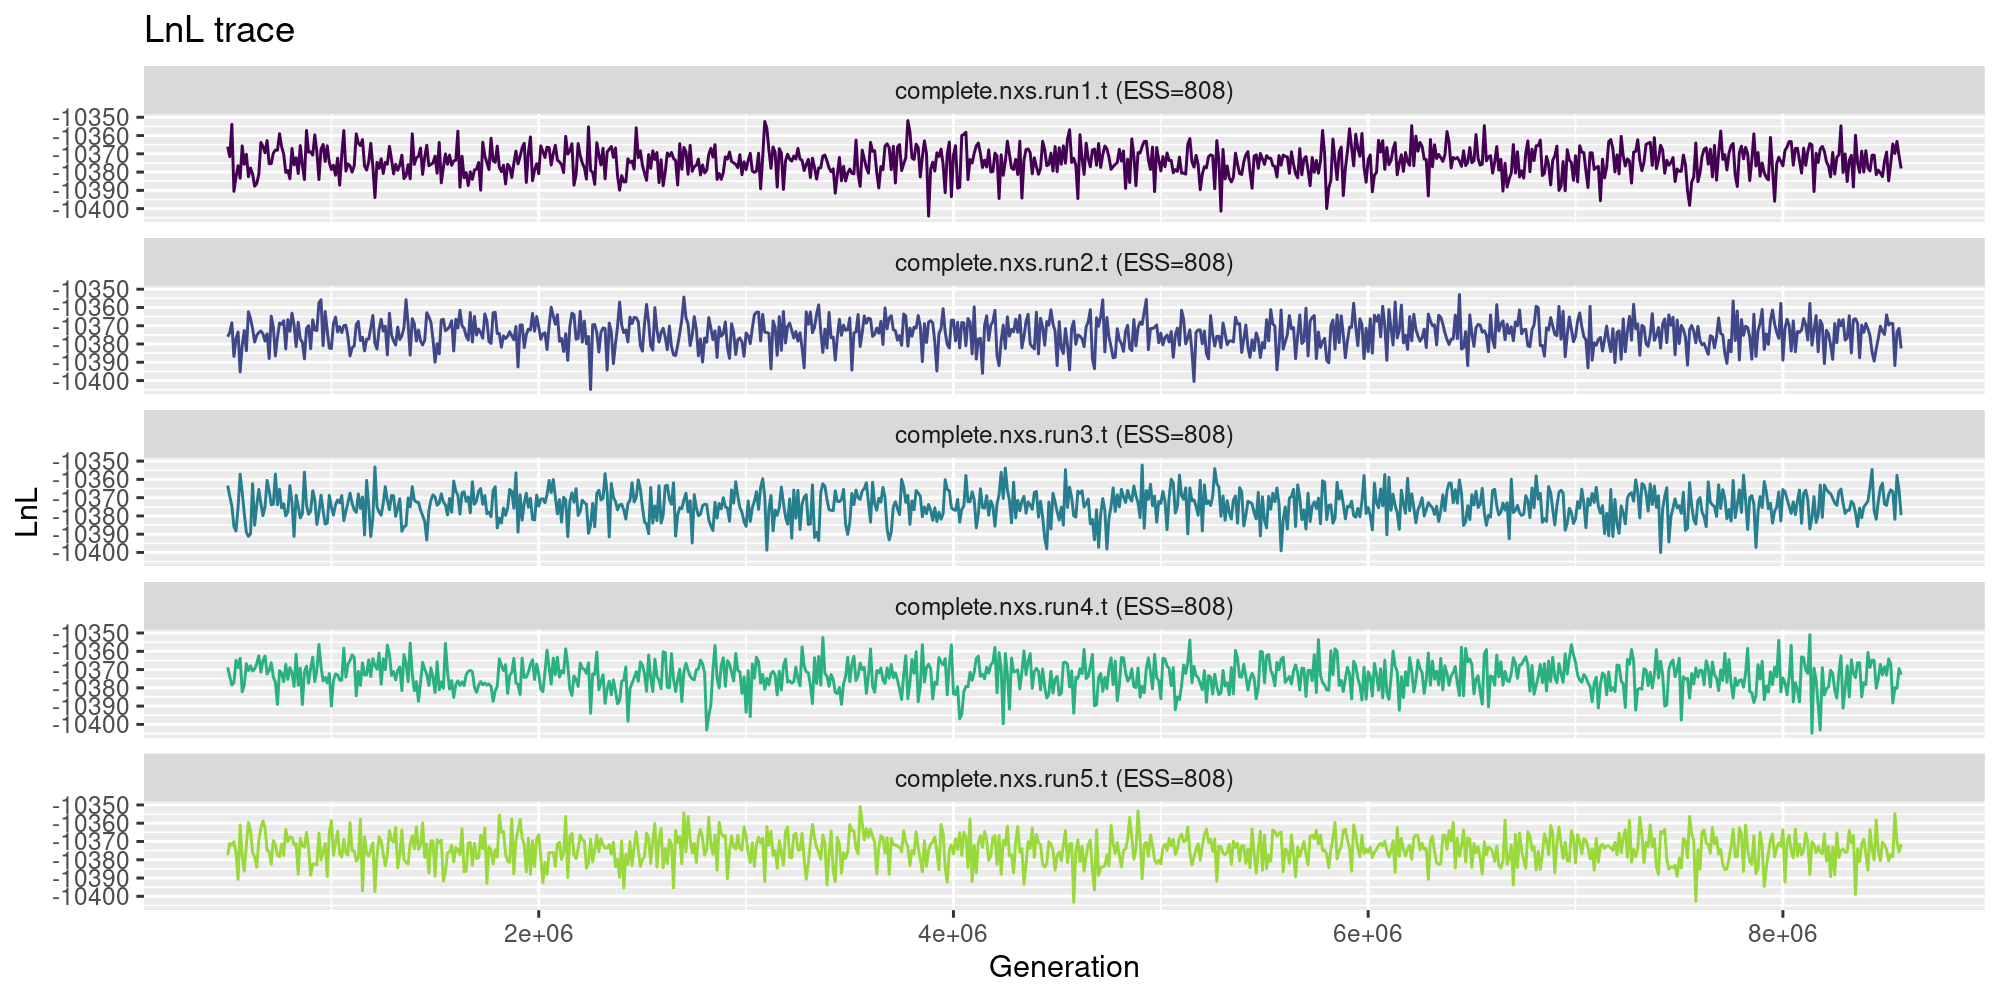
\includegraphics{LnL_trace.png}
\caption{Log likelihood trace}
\end{figure}

In the density plot we are looking to see that the values sampled by
each of the runs is approximately the same.

\begin{figure}
\centering
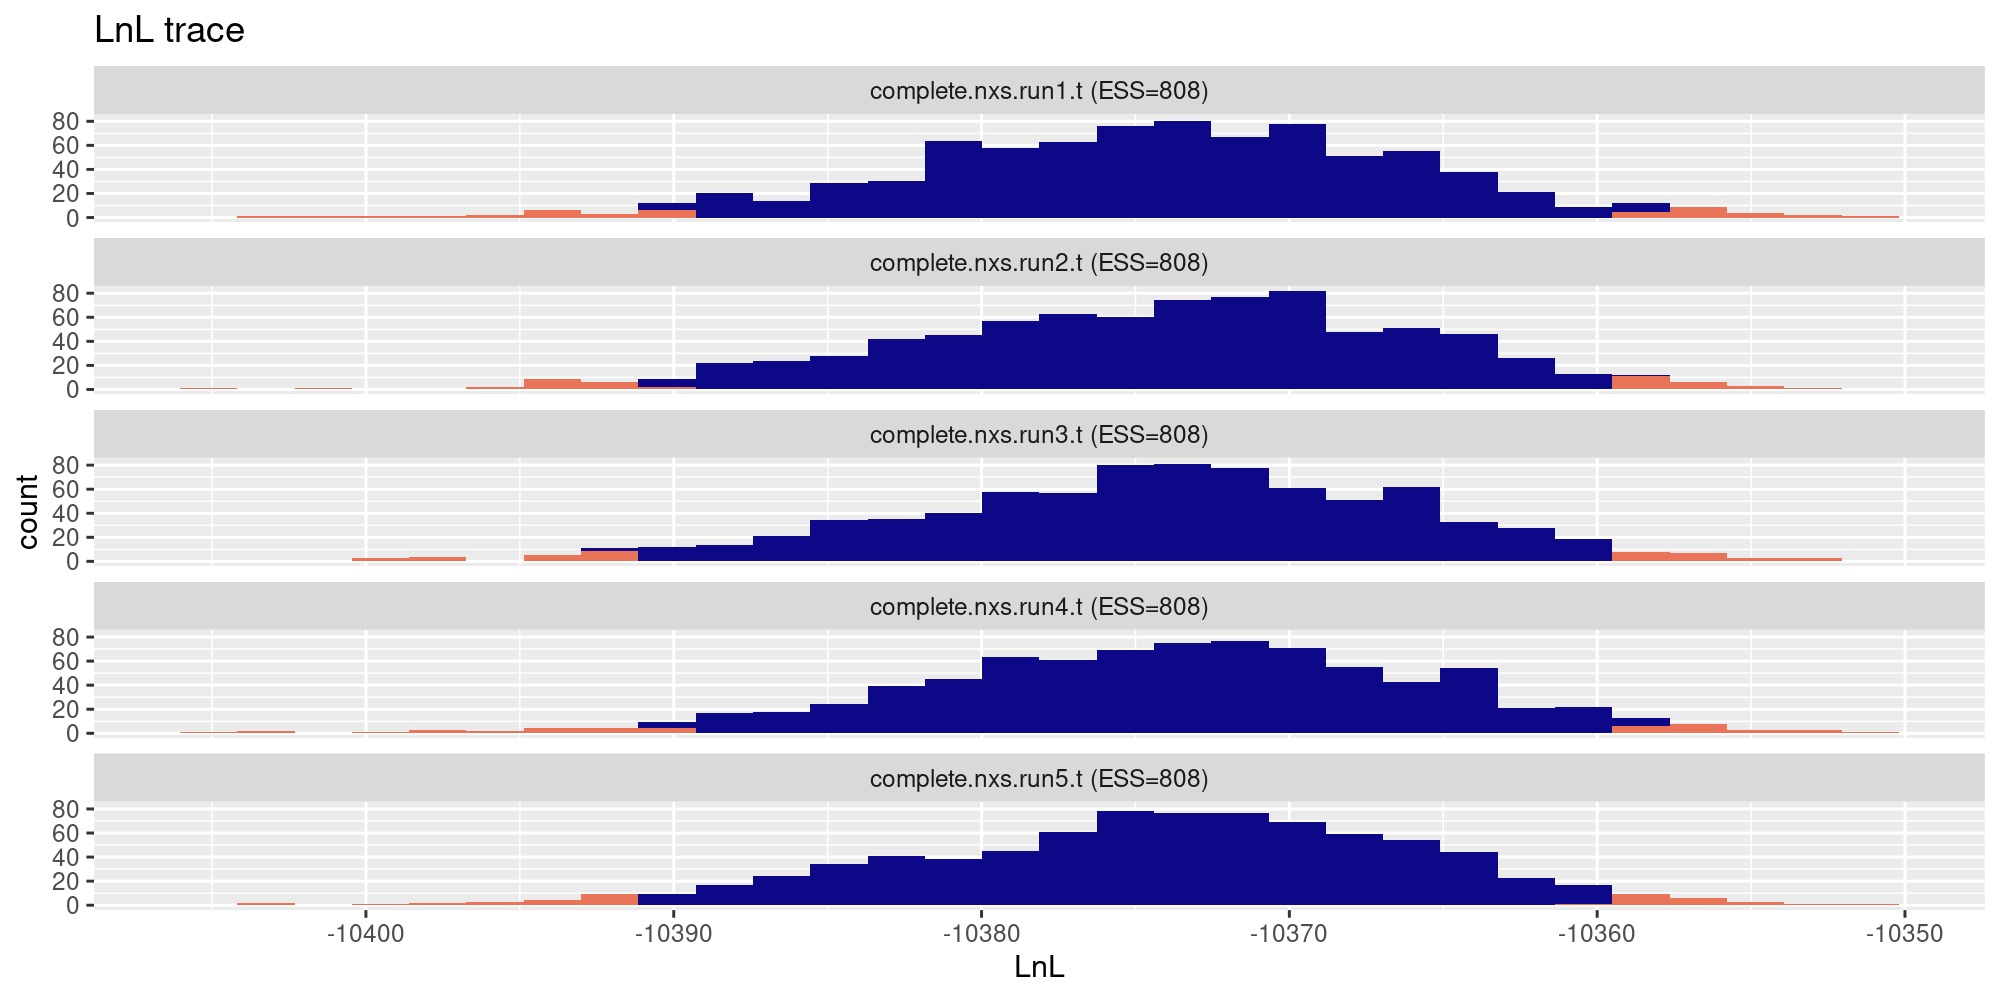
\includegraphics{LnL_density.png}
\caption{Log likelihood density plot}
\end{figure}

\hypertarget{tree-topology-plot}{%
\subsubsection{Tree topology plot}\label{tree-topology-plot}}

Tree topology trace show the difference in sampled tree topology from
the focal tree (on the y-axis) across generations of the bayesian
analysis (x-axis). According the documentation: ``Well mixed chains will
show the topology trace jumping rapidly between values. Poorly mixed
chains will show chains remaining at similar values in successive
samples. Topology traces can also reveal whether different chains are
sampling different bits of tree space, in which case the stationary
distributions will show traces at different y values on the plot.''
(\url{https://cran.r-project.org/web/packages/rwty/vignettes/rwty.html})

\begin{Shaded}
\begin{Highlighting}[]
\FunctionTok{png}\NormalTok{(}\StringTok{"Topology\_trace.png"}\NormalTok{,}\AttributeTok{width=}\DecValTok{2000}\NormalTok{,}\AttributeTok{height=}\DecValTok{1000}\NormalTok{,}\AttributeTok{res=}\DecValTok{200}\NormalTok{)}
\FunctionTok{makeplot.topology}\NormalTok{(octo.trees, }\AttributeTok{burnin =} \DecValTok{50}\NormalTok{)}\SpecialCharTok{$}\NormalTok{trace.plot}
\FunctionTok{dev.off}\NormalTok{()}
\end{Highlighting}
\end{Shaded}

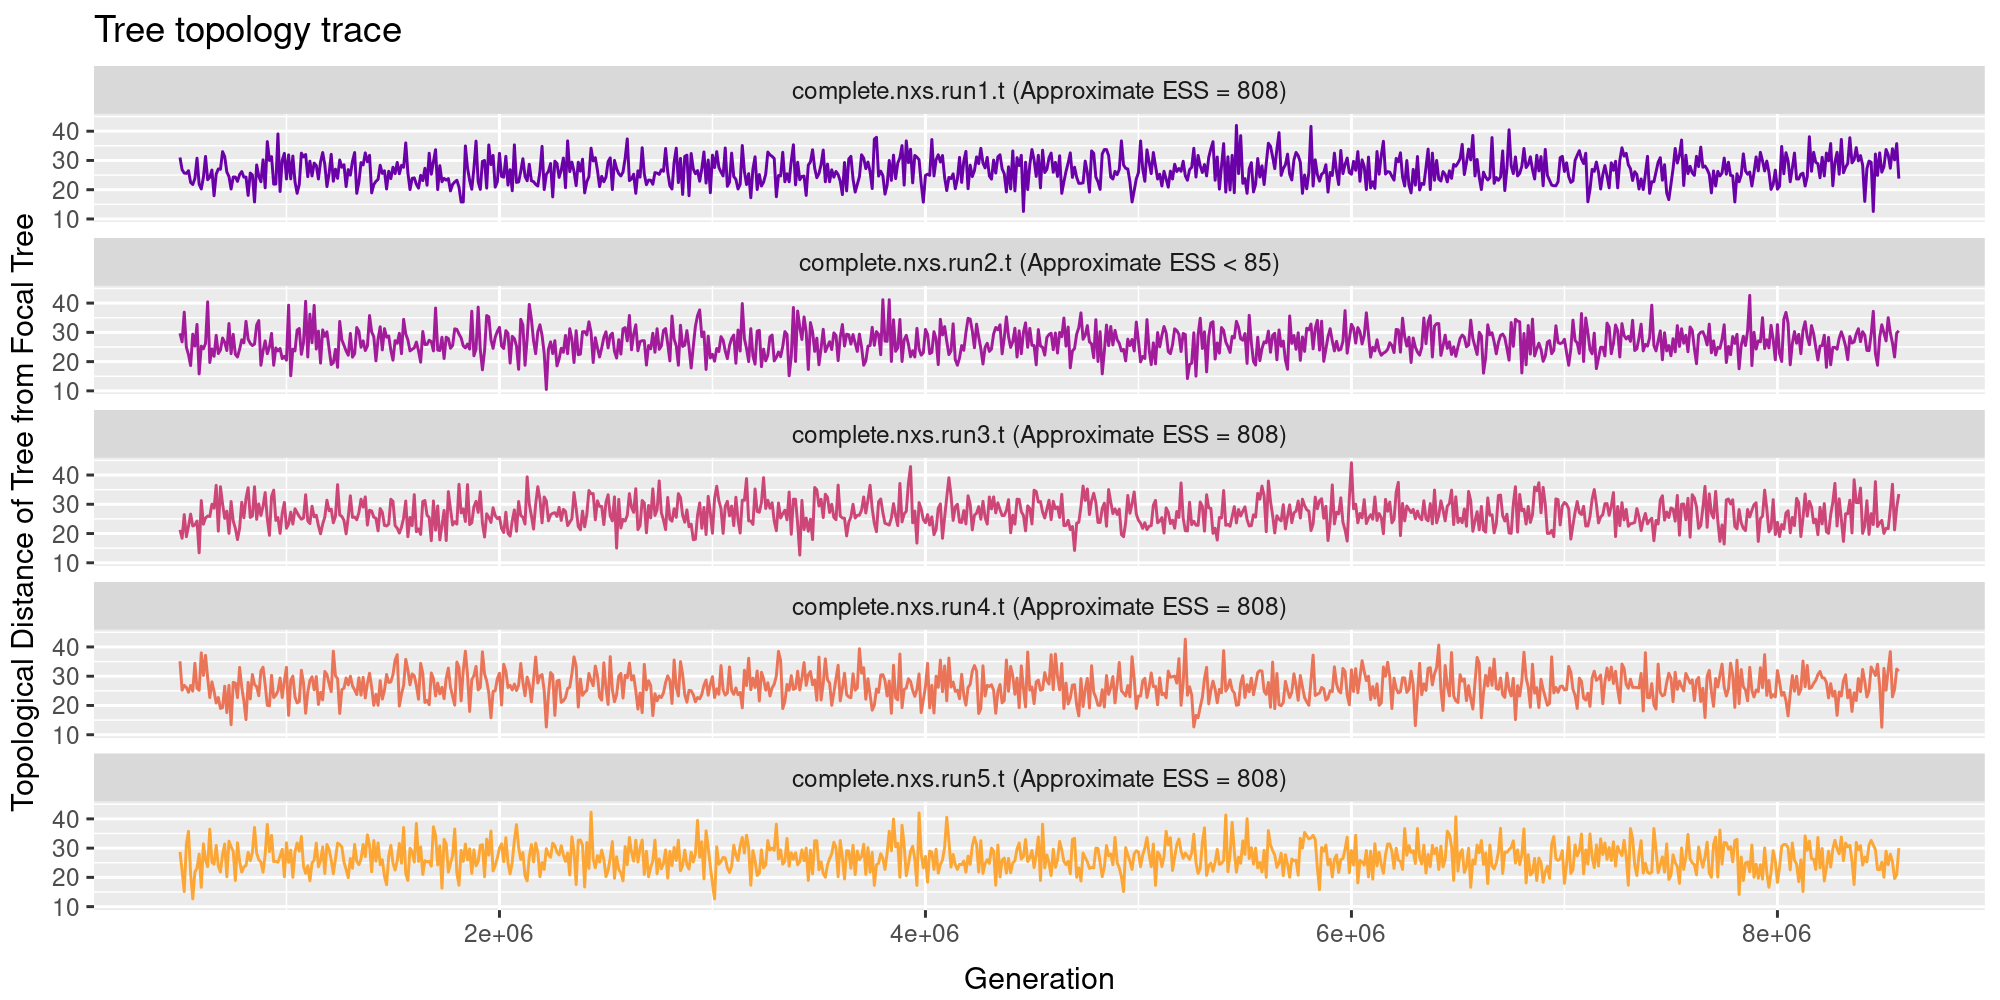
\includegraphics{Topology_trace.png} \#\#\# Split frequency plots Next
up, we look at the split frequency plots. According to the documentation
for the functions: ``In an analysis that is mixing well, we expect the
frequencies in the sliding window to move around a lot, but the
frequencies in the cumulative plot should level off. If the frequencies
in the cumulative plot have not leveled off, it might be necessary to
run the chain for longer.''

\begin{Shaded}
\begin{Highlighting}[]
\FunctionTok{png}\NormalTok{(}\StringTok{"sliding\_split\_freq.png"}\NormalTok{,}\AttributeTok{width=}\DecValTok{2000}\NormalTok{,}\AttributeTok{height=}\DecValTok{1000}\NormalTok{,}\AttributeTok{res=}\DecValTok{200}\NormalTok{)}
\FunctionTok{makeplot.splitfreqs.sliding}\NormalTok{(octo.trees, }\AttributeTok{burnin =} \DecValTok{50}\NormalTok{)}
\FunctionTok{dev.off}\NormalTok{()}
\end{Highlighting}
\end{Shaded}

\begin{figure}
\centering
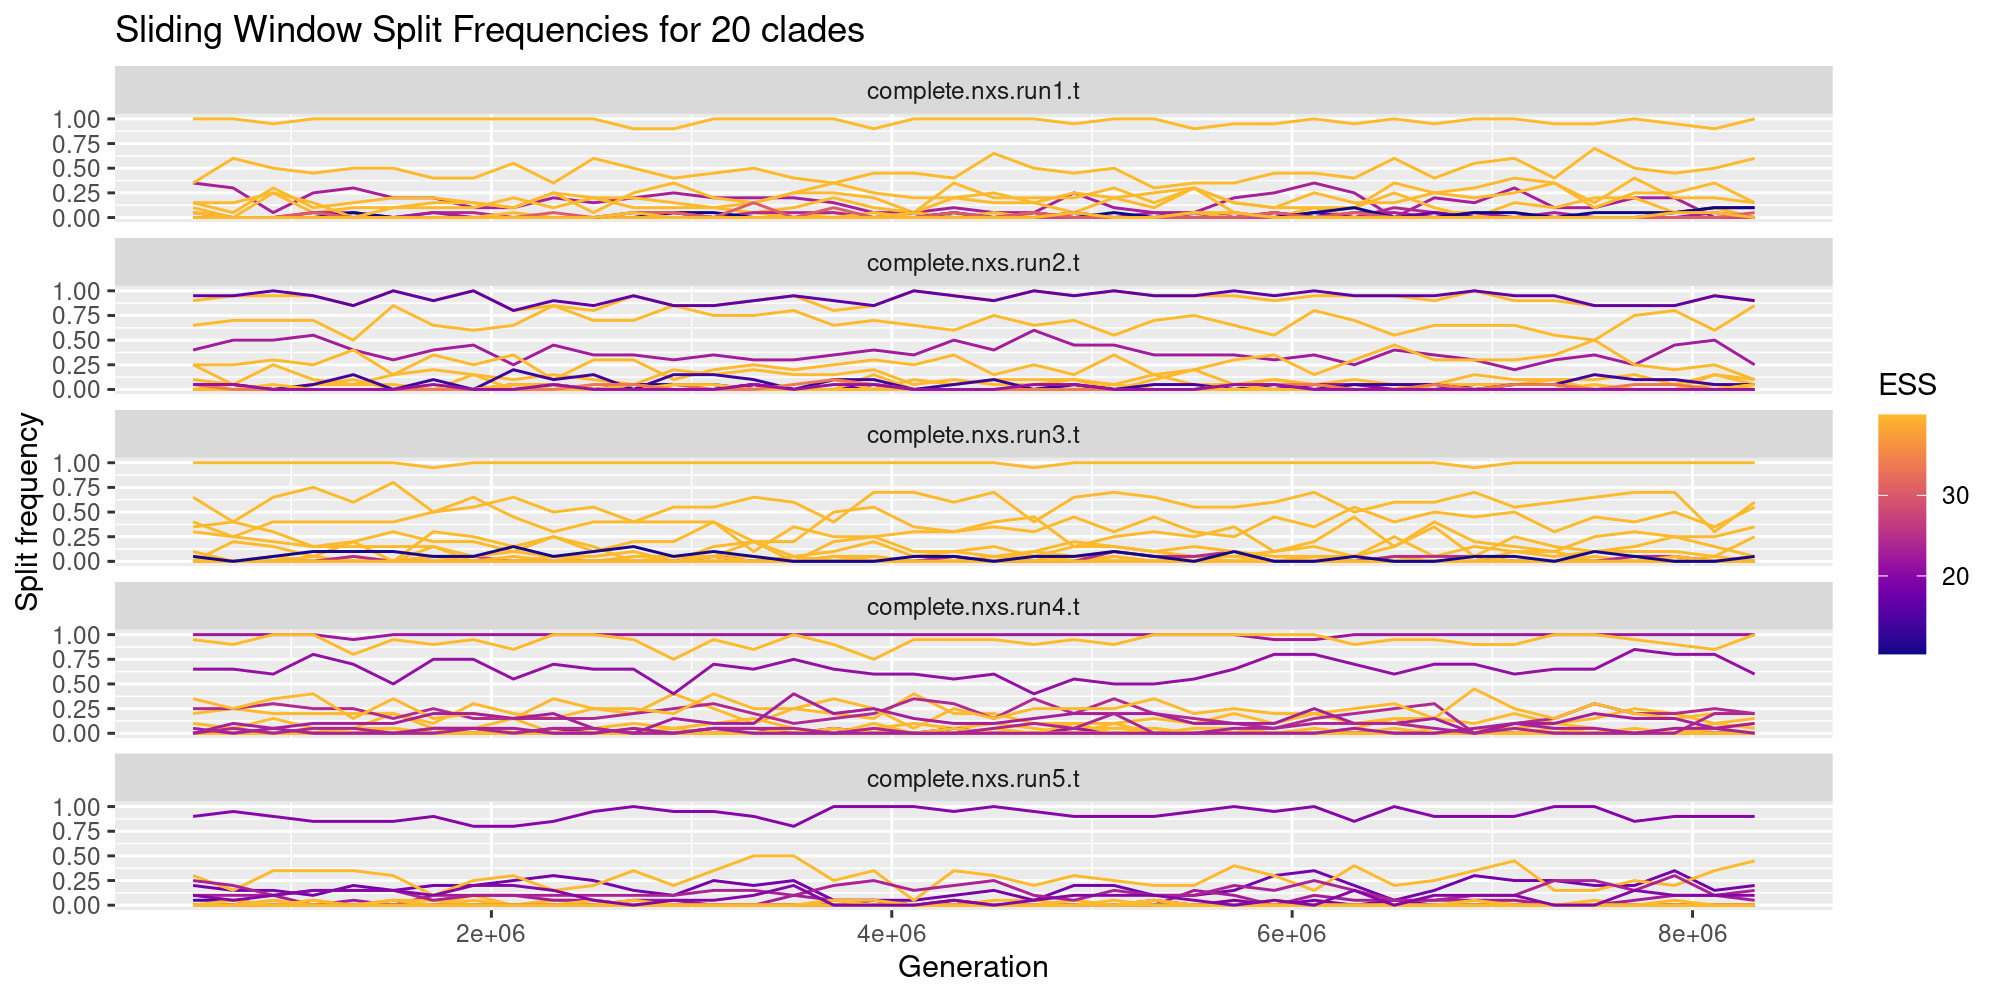
\includegraphics{sliding_split_freq.png}
\caption{Sliding Window Split Frequency Plot}
\end{figure}

\begin{Shaded}
\begin{Highlighting}[]
\FunctionTok{png}\NormalTok{(}\StringTok{"cumulative\_split\_freq.png"}\NormalTok{,}\AttributeTok{width=}\DecValTok{2000}\NormalTok{,}\AttributeTok{height=}\DecValTok{1000}\NormalTok{,}\AttributeTok{res=}\DecValTok{200}\NormalTok{)}
\FunctionTok{makeplot.splitfreqs.cumulative}\NormalTok{(octo.trees, }\AttributeTok{burnin =} \DecValTok{50}\NormalTok{)}
\FunctionTok{dev.off}\NormalTok{()}
\end{Highlighting}
\end{Shaded}

\begin{figure}
\centering
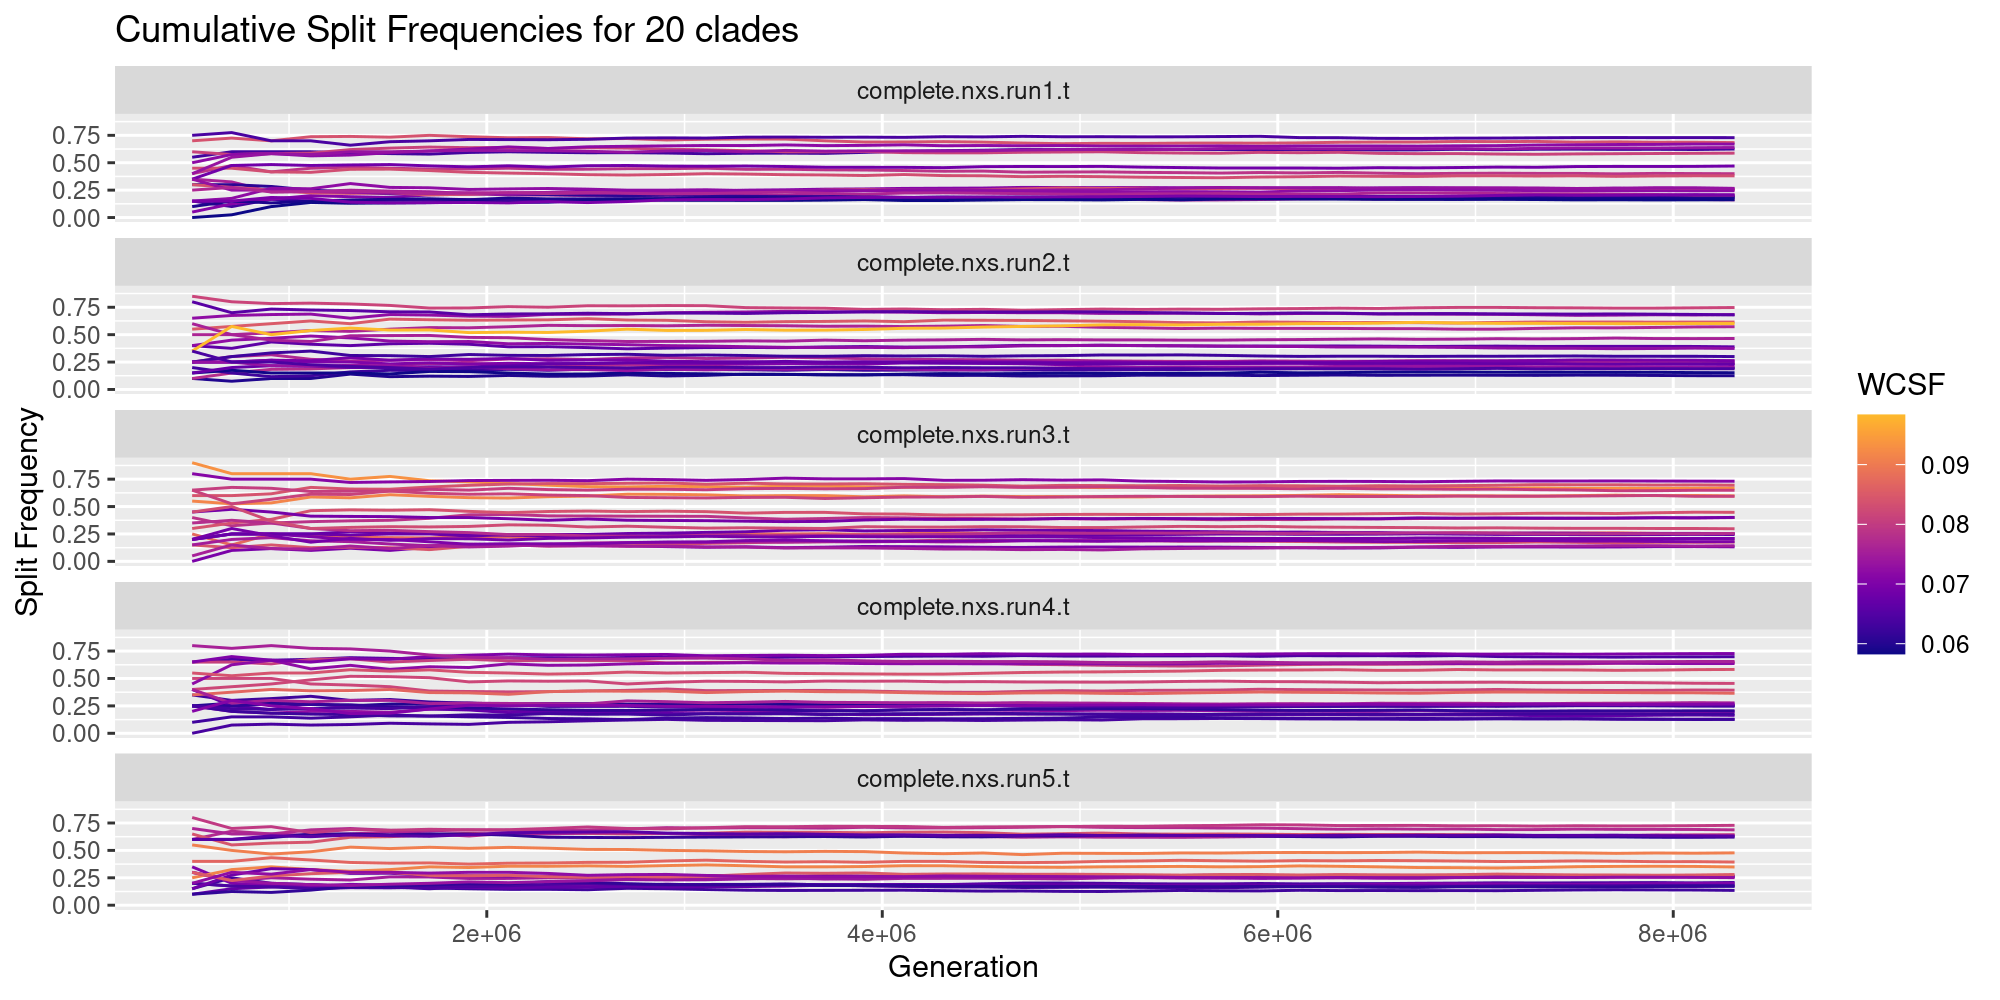
\includegraphics{cumulative_split_freq.png}
\caption{Cumulative split frequency plot}
\end{figure}

\hypertarget{tree-space-heatmap}{%
\subsubsection{Tree space heatmap}\label{tree-space-heatmap}}

This plot show the areas of treespace sampled by each run.

\begin{Shaded}
\begin{Highlighting}[]
\FunctionTok{png}\NormalTok{(}\StringTok{"treespace\_heatmap.png"}\NormalTok{,}\AttributeTok{width=}\DecValTok{2000}\NormalTok{,}\AttributeTok{height=}\DecValTok{1000}\NormalTok{,}\AttributeTok{res=}\DecValTok{200}\NormalTok{)}
\FunctionTok{makeplot.treespace}\NormalTok{(octo.trees, }\AttributeTok{burnin =}\DecValTok{50}\NormalTok{, }\AttributeTok{fill.color =} \StringTok{"LnL"}\NormalTok{)}\SpecialCharTok{$}\NormalTok{treespace.heatmap}
\FunctionTok{dev.off}\NormalTok{()}
\end{Highlighting}
\end{Shaded}

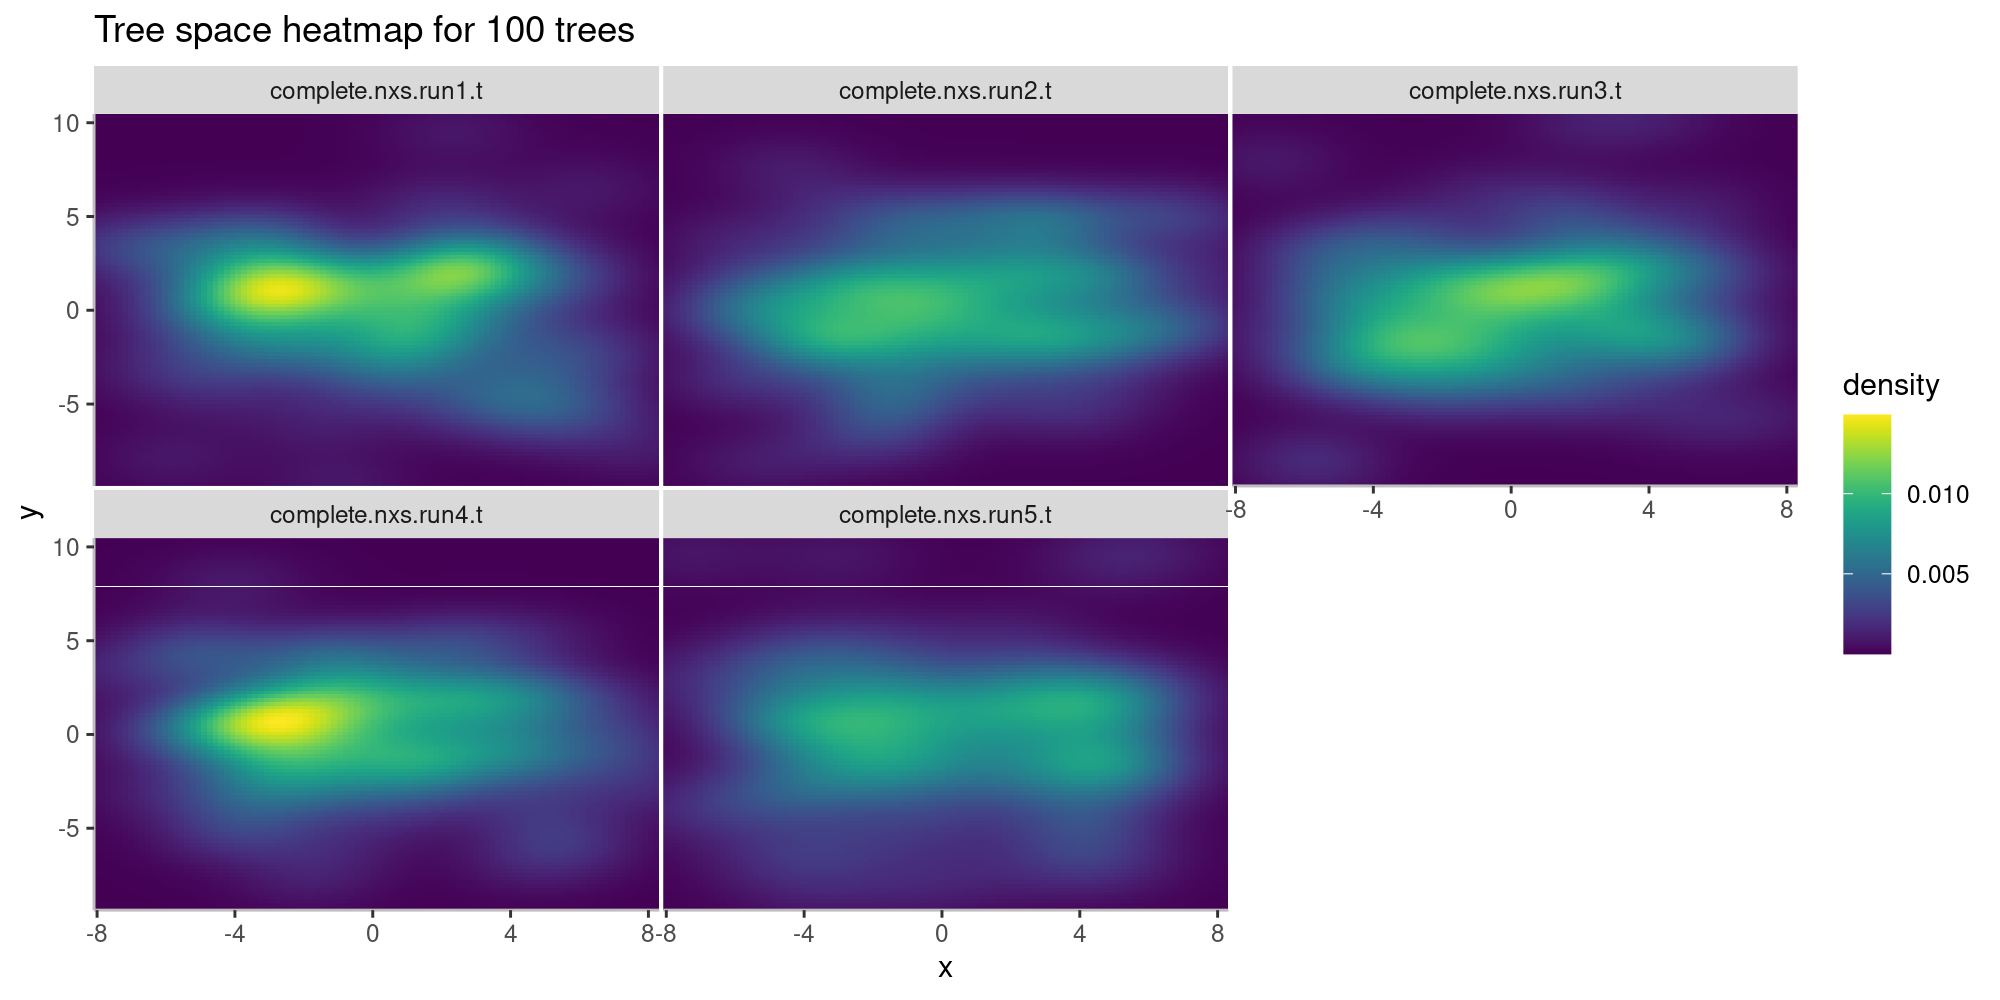
\includegraphics{treespace_heatmap.png} \#\#\# Split Frequency Matrix

\begin{Shaded}
\begin{Highlighting}[]
\FunctionTok{png}\NormalTok{(}\StringTok{"split\_freq\_matrix.png"}\NormalTok{,}\AttributeTok{width=}\DecValTok{2000}\NormalTok{,}\AttributeTok{height=}\DecValTok{1000}\NormalTok{,}\AttributeTok{res=}\DecValTok{200}\NormalTok{)}
\FunctionTok{makeplot.splitfreq.matrix}\NormalTok{(octo.trees, }\AttributeTok{burnin =} \DecValTok{50}\NormalTok{)}\SpecialCharTok{$}\NormalTok{splitfreq.matrix}
\FunctionTok{dev.off}\NormalTok{()}
\end{Highlighting}
\end{Shaded}

\begin{figure}
\centering
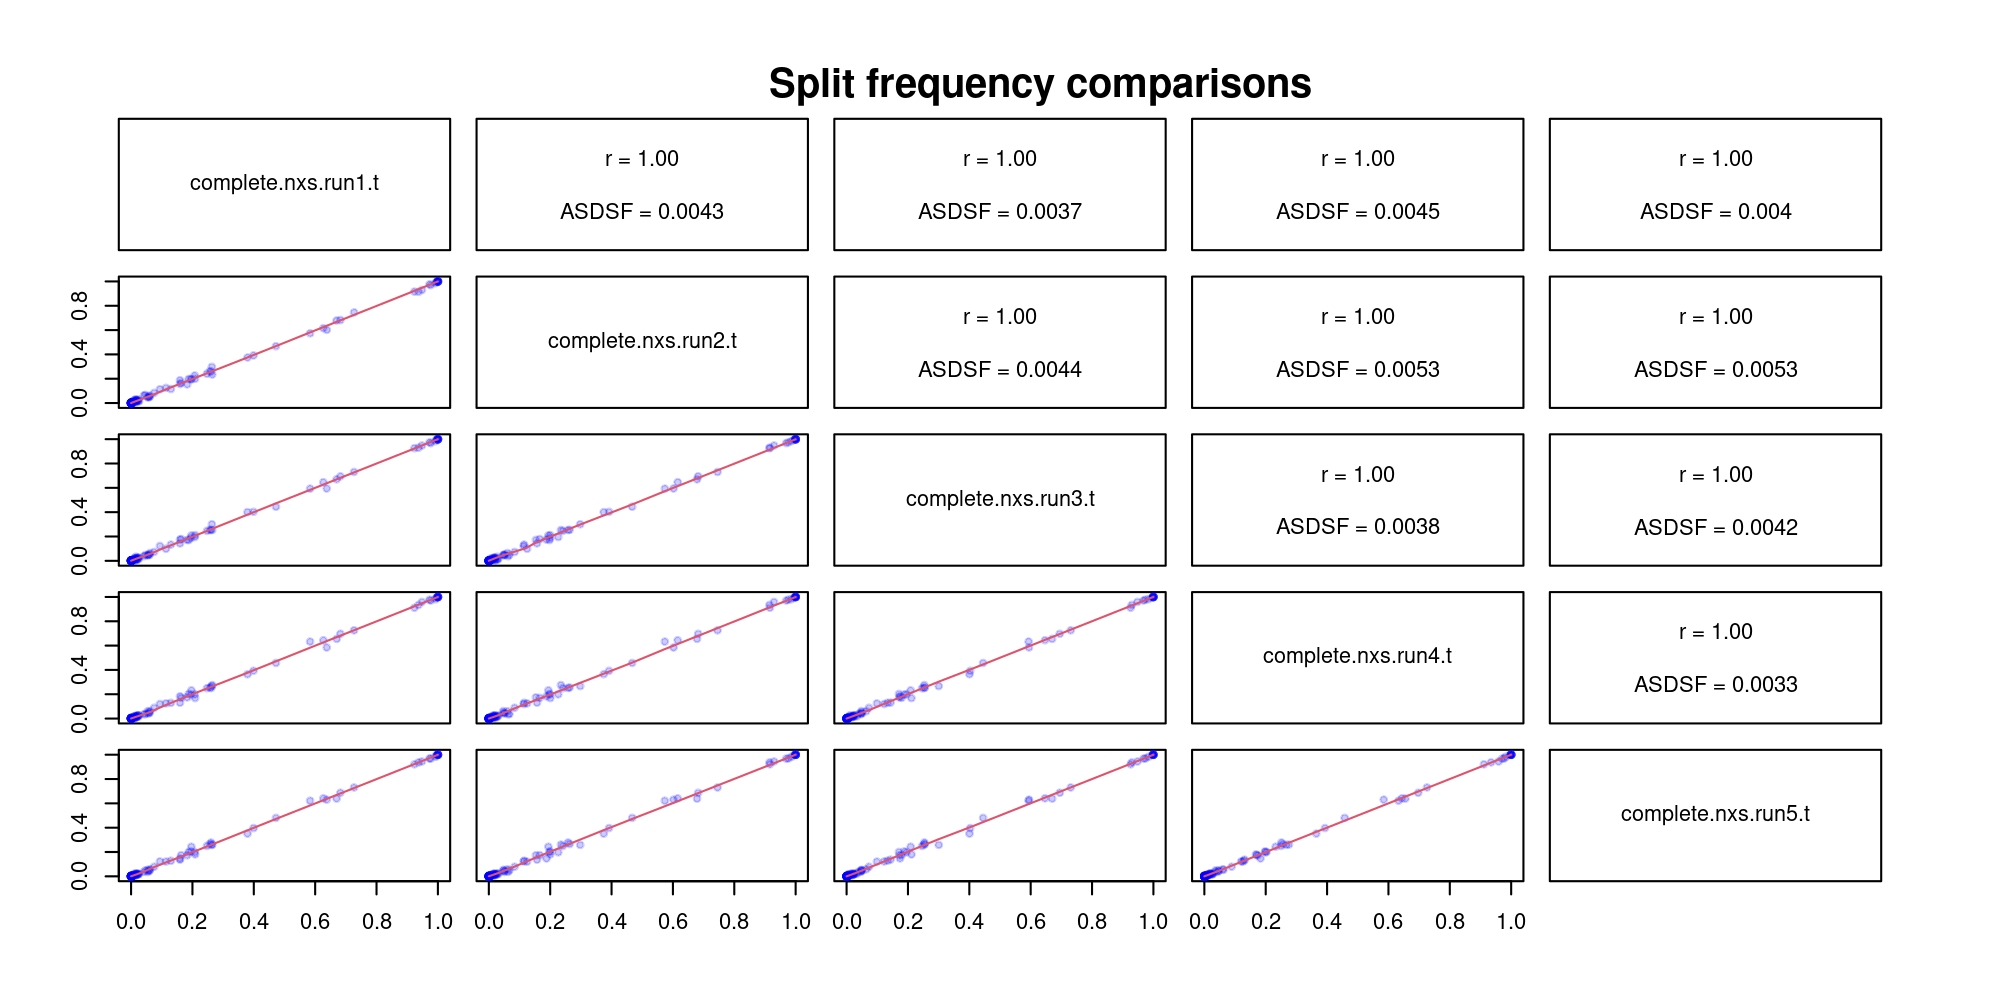
\includegraphics{split_freq_matrix.png}
\caption{Split frequency matrix plot}
\end{figure}

Finally, I am removing the octo.trees and octo.rwty object because they
are super big.

\begin{Shaded}
\begin{Highlighting}[]
\FunctionTok{rm}\NormalTok{(octo.trees)}
\end{Highlighting}
\end{Shaded}

\begin{verbatim}
## Warning in rm(octo.trees): object 'octo.trees' not found
\end{verbatim}

\begin{Shaded}
\begin{Highlighting}[]
\FunctionTok{rm}\NormalTok{(octo.rwty)}
\end{Highlighting}
\end{Shaded}

\begin{verbatim}
## Warning in rm(octo.rwty): object 'octo.rwty' not found
\end{verbatim}

\hypertarget{single-gene-trees}{%
\section{Single Gene Trees}\label{single-gene-trees}}

\hypertarget{s-only-tree}{%
\subsection{12s Only Tree}\label{s-only-tree}}

\begin{Shaded}
\begin{Highlighting}[]
\NormalTok{x12s.solo}\OtherTok{=}\NormalTok{x12s.final[}\FunctionTok{complete.cases}\NormalTok{(access}\SpecialCharTok{$}\NormalTok{X12s),]}
\FunctionTok{write.nexus.data}\NormalTok{(x12s.solo,}\StringTok{"12s\_solo.nxs"}\NormalTok{,}\AttributeTok{charsperline =} \DecValTok{1000}\NormalTok{)}
\FunctionTok{length}\NormalTok{(x12s.solo[}\DecValTok{1}\NormalTok{,])}\SpecialCharTok{+}\FunctionTok{max}\NormalTok{(}\FunctionTok{nchar}\NormalTok{(}\FunctionTok{labels}\NormalTok{(x12s.solo)))}\SpecialCharTok{+}\DecValTok{10}
\end{Highlighting}
\end{Shaded}

\begin{verbatim}
## [1] 536
\end{verbatim}

\begin{Shaded}
\begin{Highlighting}[]
\FunctionTok{sed} \AttributeTok{{-}i} \AttributeTok{{-}E} \StringTok{\textquotesingle{}s/(\^{}.\{536\}).*/\textbackslash{}1/g\textquotesingle{}}\NormalTok{ 12s\_solo.nxs}
\end{Highlighting}
\end{Shaded}

\hypertarget{writing-length-variable-lines}{%
\subsubsection{Writing length variable
lines}\label{writing-length-variable-lines}}

\begin{Shaded}
\begin{Highlighting}[]
\FunctionTok{write.table}\NormalTok{(}\FunctionTok{paste}\NormalTok{(}\StringTok{"  DIMENSIONS NTAX="}\NormalTok{,}
                  \FunctionTok{dim}\NormalTok{(x12s.solo)[}\DecValTok{1}\NormalTok{],}
                  \StringTok{" NCHAR="}\NormalTok{,}
                  \FunctionTok{dim}\NormalTok{(x12s.solo)[}\DecValTok{2}\NormalTok{],}
                  \StringTok{";"}\NormalTok{,}\AttributeTok{sep=}\StringTok{""}\NormalTok{),}
            \StringTok{"12s\_dimensions"}\NormalTok{,}
            \AttributeTok{row.names =}\NormalTok{ F,}\AttributeTok{col.names =}\NormalTok{ F,}\AttributeTok{quote =}\NormalTok{ F)}

\FunctionTok{write.table}\NormalTok{(models.muus[}\FunctionTok{grepl}\NormalTok{(}\StringTok{"}\SpecialCharTok{\textbackslash{}\textbackslash{}}\StringTok{(1}\SpecialCharTok{\textbackslash{}\textbackslash{}}\StringTok{)|}\SpecialCharTok{\textbackslash{}\textbackslash{}}\StringTok{(2}\SpecialCharTok{\textbackslash{}\textbackslash{}}\StringTok{)"}\NormalTok{,models.muus)],}
            \StringTok{"12s\_models\_to\_write"}\NormalTok{,}\AttributeTok{row.names =}\NormalTok{ F,}\AttributeTok{col.names =}\NormalTok{ F,}\AttributeTok{quote =}\NormalTok{ F)}
\end{Highlighting}
\end{Shaded}

\hypertarget{generating-nexus-file-with-mrbayes-command-block.-1}{%
\subsubsection{Generating nexus file with MrBayes command
block.}\label{generating-nexus-file-with-mrbayes-command-block.-1}}

\begin{Shaded}
\begin{Highlighting}[]
\FunctionTok{rm}\NormalTok{ 12s\_alone.nxs }\CommentTok{\#just cleaning out previous iteration if running multiple times}
\FunctionTok{cp} \AttributeTok{{-}r}\NormalTok{ mb\_12s mb\_12s.backup}
\FunctionTok{rm} \AttributeTok{{-}r}\NormalTok{ mb\_12s}
\FunctionTok{touch}\NormalTok{ 12s\_alone.nxs}
\BuiltInTok{echo} \StringTok{"\#NEXUS"} \OperatorTok{\textgreater{}\textgreater{}}\NormalTok{ 12s\_alone.nxs}
\BuiltInTok{echo} \StringTok{"BEGIN DATA;"} \OperatorTok{\textgreater{}\textgreater{}}\NormalTok{ 12s\_alone.nxs}
\FunctionTok{sed} \AttributeTok{{-}n}\NormalTok{ 1p 12s\_dimensions }\OperatorTok{\textgreater{}\textgreater{}}\NormalTok{ 12s\_alone.nxs}
\BuiltInTok{echo} \StringTok{"  FORMAT DATATYPE=DNA MISSING=? GAP={-} INTERLEAVE=YES;}
\StringTok{  MATRIX}
\StringTok{  }
\StringTok{  [12s]"} \OperatorTok{\textgreater{}\textgreater{}}\NormalTok{ 12s\_alone.nxs }
\FunctionTok{sed} \AttributeTok{{-}n}\NormalTok{ 7,96p 12s\_solo.nxs }\OperatorTok{\textgreater{}\textgreater{}}\NormalTok{ 12s\_alone.nxs}
\BuiltInTok{echo} \StringTok{"}
\StringTok{begin mrbayes;}
\StringTok{    [Define pairs for the doublet model]"} \OperatorTok{\textgreater{}\textgreater{}}\NormalTok{ 12s\_alone.nxs}
\FunctionTok{cat}\NormalTok{ basepairs }\KeywordTok{|} \FunctionTok{sed} \StringTok{\textquotesingle{}1s/\^{}/    pairs /\textquotesingle{}} \KeywordTok{|} \FunctionTok{sed} \AttributeTok{{-}E} \StringTok{\textquotesingle{}s/(:[0{-}9]\{,4\})/\textbackslash{}1,/g\textquotesingle{}} \KeywordTok{|} \FunctionTok{sed} \AttributeTok{{-}E} \StringTok{\textquotesingle{}s/,$/;/g\textquotesingle{}} \KeywordTok{|} \FunctionTok{sed} \AttributeTok{{-}r} \StringTok{\textquotesingle{}s/(.\{72,76\} )/\textbackslash{}1\textbackslash{}n         /g\textquotesingle{}} \OperatorTok{\textgreater{}\textgreater{}}\NormalTok{ 12s\_alone.nxs}
\BuiltInTok{echo} \StringTok{" "} \OperatorTok{\textgreater{}\textgreater{}}\NormalTok{ 12s\_alone.nxs}
\FunctionTok{cat}\NormalTok{ stems12s }\KeywordTok{|} \FunctionTok{sed} \StringTok{\textquotesingle{}1s/\^{}/       charset  12s{-}stems = /\textquotesingle{}} \KeywordTok{|} \FunctionTok{sed} \AttributeTok{{-}E} \StringTok{\textquotesingle{}s/$/;/g\textquotesingle{}} \KeywordTok{|} \FunctionTok{sed} \AttributeTok{{-}r} \StringTok{\textquotesingle{}s/(.\{73,76\} )/\textbackslash{}1\textbackslash{}n           /g\textquotesingle{}} \KeywordTok{|} \FunctionTok{sed} \StringTok{\textquotesingle{}1s/\^{}/\textbackslash{}n/\textquotesingle{}} \OperatorTok{\textgreater{}\textgreater{}}\NormalTok{ 12s\_alone.nxs}

\BuiltInTok{echo} \StringTok{" "} \OperatorTok{\textgreater{}\textgreater{}}\NormalTok{ 12s\_alone.nxs}
\FunctionTok{cat}\NormalTok{ loops12s }\KeywordTok{|} \FunctionTok{sed} \StringTok{\textquotesingle{}1s/\^{}/       charset  12s{-}loops = /\textquotesingle{}} \KeywordTok{|} \FunctionTok{sed} \AttributeTok{{-}E} \StringTok{\textquotesingle{}s/$/;/g\textquotesingle{}} \KeywordTok{|} \FunctionTok{sed} \AttributeTok{{-}r} \StringTok{\textquotesingle{}s/(.\{73,76\} )/\textbackslash{}1\textbackslash{}n           /g\textquotesingle{}} \KeywordTok{|} \FunctionTok{sed} \StringTok{\textquotesingle{}1s/\^{}/\textbackslash{}n/\textquotesingle{}} \OperatorTok{\textgreater{}\textgreater{}}\NormalTok{ 12s\_alone.nxs}
\BuiltInTok{echo} \StringTok{" "} \OperatorTok{\textgreater{}\textgreater{}}\NormalTok{ 12s\_alone.nxs}
\BuiltInTok{echo} \StringTok{"      partition by\_gene = 2:12s{-}stems,12s{-}loops;"} \OperatorTok{\textgreater{}\textgreater{}}\NormalTok{ 12s\_alone.nxs}
\BuiltInTok{echo} \StringTok{"      set partition = by\_gene;}
\StringTok{"} \OperatorTok{\textgreater{}\textgreater{}}\NormalTok{ 12s\_alone.nxs}
\BuiltInTok{echo} \StringTok{"      constraint outg = Octopus\_vulgaris Octopus\_rubescens Octopus\_bimaculoides Octopus\_cyanea Amphioctopus\_aegina Hapalochlaena\_maculosa Abdopus\_aculeatus Octopus\_tetricus Octopus\_berrima Macroctopus\_maorum;}
\StringTok{        prset topologypr = constraints (outg);}
\StringTok{        outgroup Octopus\_vulgaris;}
\StringTok{        "} \OperatorTok{\textgreater{}\textgreater{}}\NormalTok{ 12s\_alone.nxs}
\BuiltInTok{echo} \StringTok{"      lset applyto=(1)   nucmodel=doublet;}
\StringTok{        lset applyto=(2)   nucmodel=4by4;}
\StringTok{        prset ratepr=variable;}
\StringTok{        unlink statefreq=(all) revmat=(all) shape=(all) pinvar=(all);"} \OperatorTok{\textgreater{}\textgreater{}}\NormalTok{ 12s\_alone.nxs}

\FunctionTok{cat}\NormalTok{ 12s\_models\_to\_write }\OperatorTok{\textgreater{}\textgreater{}}\NormalTok{ 12s\_alone.nxs}

\BuiltInTok{echo} \StringTok{"}
\StringTok{      mcmcp ngen=100000000 printfreq=1000 samplefreq=10000 stoprule=yes stopval=0.01 nruns=5 nchains=2 burninfrac=0.25;}
\StringTok{      mcmc;}
\StringTok{      sump;}
\StringTok{      sumt filename=mb\_12s/12s\_alone.nxs conformat=simple;}

\StringTok{end;}
\StringTok{"} \OperatorTok{\textgreater{}\textgreater{}}\NormalTok{ 12s\_alone.nxs}

\FunctionTok{mkdir}\NormalTok{ mb\_12s}
\FunctionTok{cp}\NormalTok{ 12s\_alone.nxs mb\_12s/12s\_alone.nxs}
\end{Highlighting}
\end{Shaded}

\hypertarget{running-the-mrbayes-analysis}{%
\subsubsection{Running the MrBayes
analysis}\label{running-the-mrbayes-analysis}}

\begin{Shaded}
\begin{Highlighting}[]
\ExtensionTok{mpiexec} \AttributeTok{{-}np}\NormalTok{ 10 mb mb\_12s/12s\_alone.nxs }\OperatorTok{\textgreater{}}\NormalTok{ mb\_12s\_log}
\end{Highlighting}
\end{Shaded}

\hypertarget{coiii-only-tree}{%
\subsection{COIII Only Tree}\label{coiii-only-tree}}

\begin{Shaded}
\begin{Highlighting}[]
\NormalTok{coiii.solo}\OtherTok{=}\NormalTok{coiii.final[}\FunctionTok{complete.cases}\NormalTok{(access}\SpecialCharTok{$}\NormalTok{COIII)]}
\FunctionTok{write.nexus.data}\NormalTok{(coiii.solo,}\StringTok{"coiii\_solo.nxs"}\NormalTok{,}\AttributeTok{charsperline =} \DecValTok{1000}\NormalTok{)}
\FunctionTok{length}\NormalTok{(coiii.solo}\SpecialCharTok{$}\NormalTok{Octopus\_vulgaris)}\SpecialCharTok{+}\FunctionTok{max}\NormalTok{(}\FunctionTok{nchar}\NormalTok{(}\FunctionTok{labels}\NormalTok{(coiii.solo)))}\SpecialCharTok{+}\DecValTok{10}
\end{Highlighting}
\end{Shaded}

\begin{verbatim}
## [1] 711
\end{verbatim}

\begin{Shaded}
\begin{Highlighting}[]
\FunctionTok{sed} \AttributeTok{{-}i} \AttributeTok{{-}E} \StringTok{\textquotesingle{}s/(\^{}.\{711\}).*/\textbackslash{}1/g\textquotesingle{}}\NormalTok{ coiii\_solo.nxs}
\end{Highlighting}
\end{Shaded}

\hypertarget{writing-length-variable-lines-1}{%
\subsubsection{Writing length variable
lines}\label{writing-length-variable-lines-1}}

\begin{Shaded}
\begin{Highlighting}[]
\FunctionTok{write.table}\NormalTok{(}\FunctionTok{paste}\NormalTok{(}\StringTok{"  DIMENSIONS NTAX="}\NormalTok{,}
                  \FunctionTok{length}\NormalTok{(coiii.solo),}
                  \StringTok{" NCHAR="}\NormalTok{,}
                  \FunctionTok{length}\NormalTok{(coiii.solo}\SpecialCharTok{$}\NormalTok{Octopus\_vulgaris),}
                  \StringTok{";"}\NormalTok{,}\AttributeTok{sep=}\StringTok{""}\NormalTok{),}
            \StringTok{"coiii\_dimensions"}\NormalTok{,}
            \AttributeTok{row.names =}\NormalTok{ F,}\AttributeTok{col.names =}\NormalTok{ F,}\AttributeTok{quote =}\NormalTok{ F)}
\NormalTok{coiii.models}\OtherTok{=}\NormalTok{models.muus[}\FunctionTok{grepl}\NormalTok{(}\StringTok{"}\SpecialCharTok{\textbackslash{}\textbackslash{}}\StringTok{(3}\SpecialCharTok{\textbackslash{}\textbackslash{}}\StringTok{)|}\SpecialCharTok{\textbackslash{}\textbackslash{}}\StringTok{(4}\SpecialCharTok{\textbackslash{}\textbackslash{}}\StringTok{)|}\SpecialCharTok{\textbackslash{}\textbackslash{}}\StringTok{(5}\SpecialCharTok{\textbackslash{}\textbackslash{}}\StringTok{)"}\NormalTok{,models.muus)]}
\NormalTok{coiii.models}\OtherTok{=}\FunctionTok{gsub}\NormalTok{(}\StringTok{"}\SpecialCharTok{\textbackslash{}\textbackslash{}}\StringTok{(3}\SpecialCharTok{\textbackslash{}\textbackslash{}}\StringTok{)"}\NormalTok{,}\StringTok{"(1)"}\NormalTok{,coiii.models)}
\NormalTok{coiii.models}\OtherTok{=}\FunctionTok{gsub}\NormalTok{(}\StringTok{"}\SpecialCharTok{\textbackslash{}\textbackslash{}}\StringTok{(4}\SpecialCharTok{\textbackslash{}\textbackslash{}}\StringTok{)"}\NormalTok{,}\StringTok{"(2)"}\NormalTok{,coiii.models)}
\NormalTok{coiii.models}\OtherTok{=}\FunctionTok{gsub}\NormalTok{(}\StringTok{"}\SpecialCharTok{\textbackslash{}\textbackslash{}}\StringTok{(5}\SpecialCharTok{\textbackslash{}\textbackslash{}}\StringTok{)"}\NormalTok{,}\StringTok{"(3)"}\NormalTok{,coiii.models)}
\FunctionTok{write.table}\NormalTok{(coiii.models,}
            \StringTok{"coiii\_models\_to\_write"}\NormalTok{,}\AttributeTok{row.names =}\NormalTok{ F,}\AttributeTok{col.names =}\NormalTok{ F,}\AttributeTok{quote =}\NormalTok{ F)}

\FunctionTok{write.table}\NormalTok{(}\FunctionTok{data.frame}\NormalTok{(}\AttributeTok{models=}\FunctionTok{c}\NormalTok{(}
            \FunctionTok{paste}\NormalTok{(}\StringTok{"      charset coiii\_pos1 =  "}\NormalTok{,}\DecValTok{1}\NormalTok{,}\StringTok{" {-} "}\NormalTok{,}\FunctionTok{length}\NormalTok{(coiii.solo}\SpecialCharTok{$}\NormalTok{Octopus\_vulgaris),}\StringTok{"}\SpecialCharTok{\textbackslash{}\textbackslash{}}\StringTok{3;"}\NormalTok{,}\AttributeTok{sep=}\StringTok{""}\NormalTok{),}
            \FunctionTok{paste}\NormalTok{(}\StringTok{"      charset coiii\_pos2 =  "}\NormalTok{,}\DecValTok{2}\NormalTok{,}\StringTok{" {-} "}\NormalTok{,}\FunctionTok{length}\NormalTok{(coiii.solo}\SpecialCharTok{$}\NormalTok{Octopus\_vulgaris),}\StringTok{"}\SpecialCharTok{\textbackslash{}\textbackslash{}}\StringTok{3;"}\NormalTok{,}\AttributeTok{sep=}\StringTok{""}\NormalTok{),}
            \FunctionTok{paste}\NormalTok{(}\StringTok{"      charset coiii\_pos3 =  "}\NormalTok{,}\DecValTok{3}\NormalTok{,}\StringTok{" {-} "}\NormalTok{,}\FunctionTok{length}\NormalTok{(coiii.solo}\SpecialCharTok{$}\NormalTok{Octopus\_vulgaris),}\StringTok{"}\SpecialCharTok{\textbackslash{}\textbackslash{}}\StringTok{3;"}\NormalTok{,}\AttributeTok{sep=}\StringTok{""}\NormalTok{)}
\NormalTok{            )),}
            \StringTok{"charset.coii2"}\NormalTok{,}
            \AttributeTok{row.names =}\NormalTok{ F,}\AttributeTok{col.names =}\NormalTok{ F,}\AttributeTok{quote =}\NormalTok{ F)}
\end{Highlighting}
\end{Shaded}

\hypertarget{generating-nexus-file-with-mrbayes-command-block.-2}{%
\subsubsection{Generating nexus file with MrBayes command
block.}\label{generating-nexus-file-with-mrbayes-command-block.-2}}

\begin{Shaded}
\begin{Highlighting}[]
\FunctionTok{rm}\NormalTok{ coiii\_alone.nxs }\CommentTok{\#just cleaning out previous iteration if running multiple times}
\FunctionTok{cp} \AttributeTok{{-}r}\NormalTok{ mb\_coiii mb\_coiii.backup}
\FunctionTok{rm} \AttributeTok{{-}r}\NormalTok{ mb\_coiii}
\FunctionTok{touch}\NormalTok{ coiii\_alone.nxs}
\BuiltInTok{echo} \StringTok{"\#NEXUS"} \OperatorTok{\textgreater{}\textgreater{}}\NormalTok{ coiii\_alone.nxs}
\BuiltInTok{echo} \StringTok{"BEGIN DATA;"} \OperatorTok{\textgreater{}\textgreater{}}\NormalTok{ coiii\_alone.nxs}
\FunctionTok{sed} \AttributeTok{{-}n}\NormalTok{ 1p coiii\_dimensions }\OperatorTok{\textgreater{}\textgreater{}}\NormalTok{ coiii\_alone.nxs}
\BuiltInTok{echo} \StringTok{"  FORMAT DATATYPE=DNA MISSING=? GAP={-} INTERLEAVE=YES;}
\StringTok{  MATRIX}
\StringTok{  }
\StringTok{  [COIII]"} \OperatorTok{\textgreater{}\textgreater{}}\NormalTok{ coiii\_alone.nxs}
\FunctionTok{sed} \AttributeTok{{-}n}\NormalTok{ 7,96p coiii\_solo.nxs }\OperatorTok{\textgreater{}\textgreater{}}\NormalTok{ coiii\_alone.nxs}
\BuiltInTok{echo} \StringTok{"}
\StringTok{begin mrbayes;"} \OperatorTok{\textgreater{}\textgreater{}}\NormalTok{ coiii\_alone.nxs}
\BuiltInTok{echo} \StringTok{" "} \OperatorTok{\textgreater{}\textgreater{}}\NormalTok{ coiii\_alone.nxs}
\FunctionTok{sed} \AttributeTok{{-}n}\NormalTok{ 1,3p charset.coii2 }\OperatorTok{\textgreater{}\textgreater{}}\NormalTok{ coiii\_alone.nxs}
\BuiltInTok{echo} \StringTok{" "} \OperatorTok{\textgreater{}\textgreater{}}\NormalTok{ coiii\_alone.nxs}
\BuiltInTok{echo} \StringTok{"      partition by\_gene = 3:coiii\_pos1,coiii\_pos2,coiii\_pos3;"} \OperatorTok{\textgreater{}\textgreater{}}\NormalTok{ coiii\_alone.nxs}
\BuiltInTok{echo} \StringTok{"      set partition = by\_gene;}
\StringTok{"} \OperatorTok{\textgreater{}\textgreater{}}\NormalTok{ coiii\_alone.nxs}
\BuiltInTok{echo} \StringTok{"      constraint outg = Octopus\_vulgaris Octopus\_rubescens Octopus\_bimaculoides Octopus\_cyanea Amphioctopus\_aegina Hapalochlaena\_maculosa Abdopus\_aculeatus Octopus\_tetricus Octopus\_berrima Macroctopus\_maorum;}
\StringTok{        prset topologypr = constraints (outg);}
\StringTok{        outgroup Octopus\_vulgaris;}
\StringTok{        "} \OperatorTok{\textgreater{}\textgreater{}}\NormalTok{ coiii\_alone.nxs}
\BuiltInTok{echo} \StringTok{"      lset applyto=(all)   nucmodel=4by4;}
\StringTok{        prset ratepr=variable;}
\StringTok{        unlink statefreq=(all) revmat=(all) shape=(all) pinvar=(all);"} \OperatorTok{\textgreater{}\textgreater{}}\NormalTok{ coiii\_alone.nxs}

\FunctionTok{cat}\NormalTok{ coiii\_models\_to\_write }\OperatorTok{\textgreater{}\textgreater{}}\NormalTok{ coiii\_alone.nxs}

\BuiltInTok{echo} \StringTok{"}
\StringTok{      mcmcp ngen=100000000 printfreq=1000 samplefreq=10000 stoprule=yes stopval=0.01 nruns=5 nchains=2 burninfrac=0.25;}
\StringTok{      mcmc;}
\StringTok{      sump;}
\StringTok{      sumt filename=mb\_coiii/coiii\_alone.nxs conformat=simple;}

\StringTok{end;}
\StringTok{"} \OperatorTok{\textgreater{}\textgreater{}}\NormalTok{ coiii\_alone.nxs}

\FunctionTok{mkdir}\NormalTok{ mb\_coiii}
\FunctionTok{cp}\NormalTok{ coiii\_alone.nxs mb\_coiii/coiii\_alone.nxs}
\end{Highlighting}
\end{Shaded}

\hypertarget{running-the-mrbayes-analysis-1}{%
\subsubsection{Running the MrBayes
analysis}\label{running-the-mrbayes-analysis-1}}

\begin{Shaded}
\begin{Highlighting}[]
\ExtensionTok{mpiexec} \AttributeTok{{-}np}\NormalTok{ 10 mb mb\_coiii/coiii\_alone.nxs }\OperatorTok{\textgreater{}}\NormalTok{ mb\_coiii\_log}
\end{Highlighting}
\end{Shaded}

\hypertarget{cytb-only-tree}{%
\subsection{CytB Only Tree}\label{cytb-only-tree}}

\begin{Shaded}
\begin{Highlighting}[]
\NormalTok{cytb.solo}\OtherTok{=}\NormalTok{cytb.final[}\FunctionTok{complete.cases}\NormalTok{(access}\SpecialCharTok{$}\NormalTok{Cytb)]}
\FunctionTok{write.nexus.data}\NormalTok{(cytb.solo,}\StringTok{"cytb\_solo.nxs"}\NormalTok{,}\AttributeTok{charsperline =} \DecValTok{1000}\NormalTok{)}
\FunctionTok{length}\NormalTok{(cytb.solo}\SpecialCharTok{$}\NormalTok{Octopus\_vulgaris)}\SpecialCharTok{+}\FunctionTok{max}\NormalTok{(}\FunctionTok{nchar}\NormalTok{(}\FunctionTok{labels}\NormalTok{(cytb.solo)))}\SpecialCharTok{+}\DecValTok{10}
\end{Highlighting}
\end{Shaded}

\begin{verbatim}
## [1] 675
\end{verbatim}

\begin{Shaded}
\begin{Highlighting}[]
\FunctionTok{sed} \AttributeTok{{-}i} \AttributeTok{{-}E} \StringTok{\textquotesingle{}s/(\^{}.\{675\}).*/\textbackslash{}1/g\textquotesingle{}}\NormalTok{ cytb\_solo.nxs}
\end{Highlighting}
\end{Shaded}

\hypertarget{writing-length-variable-lines-2}{%
\subsubsection{Writing length variable
lines}\label{writing-length-variable-lines-2}}

\begin{Shaded}
\begin{Highlighting}[]
\FunctionTok{write.table}\NormalTok{(}\FunctionTok{paste}\NormalTok{(}\StringTok{"  DIMENSIONS NTAX="}\NormalTok{,}
                  \FunctionTok{length}\NormalTok{(cytb.solo),}
                  \StringTok{" NCHAR="}\NormalTok{,}
                  \FunctionTok{length}\NormalTok{(cytb.solo}\SpecialCharTok{$}\NormalTok{Octopus\_vulgaris),}
                  \StringTok{";"}\NormalTok{,}\AttributeTok{sep=}\StringTok{""}\NormalTok{),}
            \StringTok{"cytb\_dimensions"}\NormalTok{,}
            \AttributeTok{row.names =}\NormalTok{ F,}\AttributeTok{col.names =}\NormalTok{ F,}\AttributeTok{quote =}\NormalTok{ F)}
\NormalTok{cytb.models}\OtherTok{=}\NormalTok{models.muus[}\FunctionTok{grepl}\NormalTok{(}\StringTok{"}\SpecialCharTok{\textbackslash{}\textbackslash{}}\StringTok{(6}\SpecialCharTok{\textbackslash{}\textbackslash{}}\StringTok{)|}\SpecialCharTok{\textbackslash{}\textbackslash{}}\StringTok{(7}\SpecialCharTok{\textbackslash{}\textbackslash{}}\StringTok{)|}\SpecialCharTok{\textbackslash{}\textbackslash{}}\StringTok{(8}\SpecialCharTok{\textbackslash{}\textbackslash{}}\StringTok{)"}\NormalTok{,models.muus)]}
\NormalTok{cytb.models}\OtherTok{=}\FunctionTok{gsub}\NormalTok{(}\StringTok{"}\SpecialCharTok{\textbackslash{}\textbackslash{}}\StringTok{(6}\SpecialCharTok{\textbackslash{}\textbackslash{}}\StringTok{)"}\NormalTok{,}\StringTok{"(1)"}\NormalTok{,cytb.models)}
\NormalTok{cytb.models}\OtherTok{=}\FunctionTok{gsub}\NormalTok{(}\StringTok{"}\SpecialCharTok{\textbackslash{}\textbackslash{}}\StringTok{(7}\SpecialCharTok{\textbackslash{}\textbackslash{}}\StringTok{)"}\NormalTok{,}\StringTok{"(2)"}\NormalTok{,cytb.models)}
\NormalTok{cytb.models}\OtherTok{=}\FunctionTok{gsub}\NormalTok{(}\StringTok{"}\SpecialCharTok{\textbackslash{}\textbackslash{}}\StringTok{(8}\SpecialCharTok{\textbackslash{}\textbackslash{}}\StringTok{)"}\NormalTok{,}\StringTok{"(3)"}\NormalTok{,cytb.models)}
\FunctionTok{write.table}\NormalTok{(cytb.models,}
            \StringTok{"cytb\_models\_to\_write"}\NormalTok{,}\AttributeTok{row.names =}\NormalTok{ F,}\AttributeTok{col.names =}\NormalTok{ F,}\AttributeTok{quote =}\NormalTok{ F)}

\FunctionTok{write.table}\NormalTok{(}\FunctionTok{data.frame}\NormalTok{(}\AttributeTok{models=}\FunctionTok{c}\NormalTok{(}
            \FunctionTok{paste}\NormalTok{(}\StringTok{"      charset cytb\_pos1 =  "}\NormalTok{,}\DecValTok{1}\NormalTok{,}\StringTok{" {-} "}\NormalTok{,}\FunctionTok{length}\NormalTok{(cytb.solo}\SpecialCharTok{$}\NormalTok{Octopus\_vulgaris),}\StringTok{"}\SpecialCharTok{\textbackslash{}\textbackslash{}}\StringTok{3;"}\NormalTok{,}\AttributeTok{sep=}\StringTok{""}\NormalTok{),}
            \FunctionTok{paste}\NormalTok{(}\StringTok{"      charset cytb\_pos2 =  "}\NormalTok{,}\DecValTok{2}\NormalTok{,}\StringTok{" {-} "}\NormalTok{,}\FunctionTok{length}\NormalTok{(cytb.solo}\SpecialCharTok{$}\NormalTok{Octopus\_vulgaris),}\StringTok{"}\SpecialCharTok{\textbackslash{}\textbackslash{}}\StringTok{3;"}\NormalTok{,}\AttributeTok{sep=}\StringTok{""}\NormalTok{),}
            \FunctionTok{paste}\NormalTok{(}\StringTok{"      charset cytb\_pos3 =  "}\NormalTok{,}\DecValTok{3}\NormalTok{,}\StringTok{" {-} "}\NormalTok{,}\FunctionTok{length}\NormalTok{(cytb.solo}\SpecialCharTok{$}\NormalTok{Octopus\_vulgaris),}\StringTok{"}\SpecialCharTok{\textbackslash{}\textbackslash{}}\StringTok{3;"}\NormalTok{,}\AttributeTok{sep=}\StringTok{""}\NormalTok{)}
\NormalTok{            )),}
            \StringTok{"charset.cytb2"}\NormalTok{,}
            \AttributeTok{row.names =}\NormalTok{ F,}\AttributeTok{col.names =}\NormalTok{ F,}\AttributeTok{quote =}\NormalTok{ F)}
\end{Highlighting}
\end{Shaded}

\hypertarget{generating-nexus-file-with-mrbayes-command-block.-3}{%
\subsubsection{Generating nexus file with MrBayes command
block.}\label{generating-nexus-file-with-mrbayes-command-block.-3}}

\begin{Shaded}
\begin{Highlighting}[]
\FunctionTok{rm}\NormalTok{ cytb\_alone.nxs }\CommentTok{\#just cleaning out previous iteration if running multiple times}
\FunctionTok{cp} \AttributeTok{{-}r}\NormalTok{ mb\_cytb mb\_cytb.backup}
\FunctionTok{rm} \AttributeTok{{-}r}\NormalTok{ mb\_cytb}
\FunctionTok{touch}\NormalTok{ cytb\_alone.nxs}
\BuiltInTok{echo} \StringTok{"\#NEXUS"} \OperatorTok{\textgreater{}\textgreater{}}\NormalTok{ cytb\_alone.nxs}
\BuiltInTok{echo} \StringTok{"BEGIN DATA;"} \OperatorTok{\textgreater{}\textgreater{}}\NormalTok{ cytb\_alone.nxs}
\FunctionTok{sed} \AttributeTok{{-}n}\NormalTok{ 1p cytb\_dimensions }\OperatorTok{\textgreater{}\textgreater{}}\NormalTok{ cytb\_alone.nxs}
\BuiltInTok{echo} \StringTok{"  FORMAT DATATYPE=DNA MISSING=? GAP={-} INTERLEAVE=YES;}
\StringTok{  MATRIX}
\StringTok{  }
\StringTok{  [Cytb]"} \OperatorTok{\textgreater{}\textgreater{}}\NormalTok{ cytb\_alone.nxs}
\FunctionTok{sed} \AttributeTok{{-}n}\NormalTok{ 7,98p cytb\_solo.nxs }\OperatorTok{\textgreater{}\textgreater{}}\NormalTok{ cytb\_alone.nxs}
\BuiltInTok{echo} \StringTok{"}
\StringTok{begin mrbayes;"} \OperatorTok{\textgreater{}\textgreater{}}\NormalTok{ cytb\_alone.nxs}
\BuiltInTok{echo} \StringTok{" "} \OperatorTok{\textgreater{}\textgreater{}}\NormalTok{ cytb\_alone.nxs}
\FunctionTok{sed} \AttributeTok{{-}n}\NormalTok{ 1,3p charset.cytb2 }\OperatorTok{\textgreater{}\textgreater{}}\NormalTok{ cytb\_alone.nxs}
\BuiltInTok{echo} \StringTok{" "} \OperatorTok{\textgreater{}\textgreater{}}\NormalTok{ cytb\_alone.nxs}
\BuiltInTok{echo} \StringTok{"      partition by\_gene = 3:cytb\_pos1,cytb\_pos2,cytb\_pos3;"} \OperatorTok{\textgreater{}\textgreater{}}\NormalTok{ cytb\_alone.nxs}
\BuiltInTok{echo} \StringTok{"      set partition = by\_gene;}
\StringTok{"} \OperatorTok{\textgreater{}\textgreater{}}\NormalTok{ cytb\_alone.nxs}
\BuiltInTok{echo} \StringTok{"      constraint outg = Octopus\_vulgaris Octopus\_bimaculoides Octopus\_cyanea Amphioctopus\_aegina Hapalochlaena\_maculosa Abdopus\_aculeatus Octopus\_tetricus Octopus\_berrima Macroctopus\_maorum;}
\StringTok{        prset topologypr = constraints (outg);}
\StringTok{        outgroup Octopus\_vulgaris;}
\StringTok{        "} \OperatorTok{\textgreater{}\textgreater{}}\NormalTok{ cytb\_alone.nxs}
\BuiltInTok{echo} \StringTok{"      lset applyto=(all)   nucmodel=4by4;}
\StringTok{        prset ratepr=variable;}
\StringTok{        unlink statefreq=(all) revmat=(all) shape=(all) pinvar=(all);"} \OperatorTok{\textgreater{}\textgreater{}}\NormalTok{ cytb\_alone.nxs}

\FunctionTok{cat}\NormalTok{ cytb\_models\_to\_write }\OperatorTok{\textgreater{}\textgreater{}}\NormalTok{ cytb\_alone.nxs}

\BuiltInTok{echo} \StringTok{"}
\StringTok{      mcmcp ngen=100000000 printfreq=1000 samplefreq=10000 stoprule=yes stopval=0.01 nruns=5 nchains=2 burninfrac=0.25;}
\StringTok{      mcmc;}
\StringTok{      sump;}
\StringTok{      sumt filename=mb\_cytb/cytb\_alone.nxs conformat=simple;}

\StringTok{end;}
\StringTok{"} \OperatorTok{\textgreater{}\textgreater{}}\NormalTok{ cytb\_alone.nxs}

\FunctionTok{mkdir}\NormalTok{ mb\_cytb}
\FunctionTok{cp}\NormalTok{ cytb\_alone.nxs mb\_cytb/cytb\_alone.nxs}
\end{Highlighting}
\end{Shaded}

\hypertarget{running-the-mrbayes-analysis-2}{%
\subsubsection{Running the MrBayes
analysis}\label{running-the-mrbayes-analysis-2}}

\begin{Shaded}
\begin{Highlighting}[]
\ExtensionTok{mpiexec} \AttributeTok{{-}np}\NormalTok{ 10 mb mb\_cytb/cytb\_alone.nxs }\OperatorTok{\textgreater{}}\NormalTok{ mb\_cytb\_log}
\end{Highlighting}
\end{Shaded}

\hypertarget{reading-into-r-the-resulting-trees}{%
\section{Reading into R the resulting
trees}\label{reading-into-r-the-resulting-trees}}

\hypertarget{reading-in-the-multi-gene-tree}{%
\subsection{Reading in the multi-gene
tree}\label{reading-in-the-multi-gene-tree}}

The file that contains the consensus trees is ``complete.nxs.con.tre''.
This file actually contains two trees. One contains no branch
probability information, and the other contains the branch
probabilities. The following code deletes the tree without probabilities
from file. If both trees are present, R opens the tree as a multi-phylo
class, and manipulation of the tree becomes much harder.

\begin{Shaded}
\begin{Highlighting}[]
\FunctionTok{cp}\NormalTok{ ./mb/complete.nxs.con.tre ./mb/completeBACKUP.nxs.con.tre}
\FunctionTok{sed} \AttributeTok{{-}i} \StringTok{\textquotesingle{}/Note: This tree contains information only on the topology/d\textquotesingle{}}\NormalTok{ ./mb/complete.nxs.con.tre}
\FunctionTok{sed} \AttributeTok{{-}i} \StringTok{\textquotesingle{}/and branch lengths (median of the posterior probability density)/d\textquotesingle{}}\NormalTok{ ./mb/complete.nxs.con.tre}
\FunctionTok{sed} \AttributeTok{{-}i} \StringTok{\textquotesingle{}/):/d\textquotesingle{}}\NormalTok{ ./mb/complete.nxs.con.tre}
\end{Highlighting}
\end{Shaded}

Now I read the tree into R using the following code.

\begin{Shaded}
\begin{Highlighting}[]
\NormalTok{mrbayes.tree}\OtherTok{=}\FunctionTok{read.nexus}\NormalTok{(}\StringTok{"mb/complete.nxs.con.tre"}\NormalTok{,}\AttributeTok{tree.names=}\ConstantTok{NULL}\NormalTok{)}
\end{Highlighting}
\end{Shaded}

\hypertarget{reading-the-12s-tree}{%
\subsection{Reading the 12s tree}\label{reading-the-12s-tree}}

Now the same or the 12s tree

\begin{Shaded}
\begin{Highlighting}[]
\FunctionTok{cp}\NormalTok{ ./mb\_12s/12s\_alone.nxs.con.tre ./mb\_12s/12s\_aloneBACKUP.nxs.con.tre}
\FunctionTok{sed} \AttributeTok{{-}i} \StringTok{\textquotesingle{}/Note: This tree contains information only on the topology/d\textquotesingle{}}\NormalTok{ ./mb\_12s/12s\_alone.nxs.con.tre}
\FunctionTok{sed} \AttributeTok{{-}i} \StringTok{\textquotesingle{}/and branch lengths (median of the posterior probability density)/d\textquotesingle{}}\NormalTok{ ./mb\_12s/12s\_alone.nxs.con.tre}
\FunctionTok{sed} \AttributeTok{{-}i} \StringTok{\textquotesingle{}/):/d\textquotesingle{}}\NormalTok{ ./mb\_12s/12s\_alone.nxs.con.tre}
\end{Highlighting}
\end{Shaded}

Now I read the tree into R using the following code.

\begin{Shaded}
\begin{Highlighting}[]
\NormalTok{x12s.tree}\OtherTok{=}\FunctionTok{read.nexus}\NormalTok{(}\StringTok{"mb\_12s/12s\_alone.nxs.con.tre"}\NormalTok{,}\AttributeTok{tree.names=}\ConstantTok{NULL}\NormalTok{)}
\end{Highlighting}
\end{Shaded}

\hypertarget{reading-the-coiii-tree}{%
\subsection{Reading the COIII tree}\label{reading-the-coiii-tree}}

Now the same or the coiii tree

\begin{Shaded}
\begin{Highlighting}[]
\FunctionTok{cp}\NormalTok{ ./mb\_coiii/coiii\_alone.nxs.con.tre ./mb\_coiii/coiii\_aloneBACKUP.nxs.con.tre}
\FunctionTok{sed} \AttributeTok{{-}i} \StringTok{\textquotesingle{}/Note: This tree contains information only on the topology/d\textquotesingle{}}\NormalTok{ ./mb\_coiii/coiii\_alone.nxs.con.tre}
\FunctionTok{sed} \AttributeTok{{-}i} \StringTok{\textquotesingle{}/and branch lengths (median of the posterior probability density)/d\textquotesingle{}}\NormalTok{ ./mb\_coiii/coiii\_alone.nxs.con.tre}
\FunctionTok{sed} \AttributeTok{{-}i} \StringTok{\textquotesingle{}/):/d\textquotesingle{}}\NormalTok{ ./mb\_coiii/coiii\_alone.nxs.con.tre}
\end{Highlighting}
\end{Shaded}

Now I read the tree into R using the following code.

\begin{Shaded}
\begin{Highlighting}[]
\NormalTok{coiii.tree}\OtherTok{=}\FunctionTok{read.nexus}\NormalTok{(}\StringTok{"mb\_coiii/coiii\_alone.nxs.con.tre"}\NormalTok{,}\AttributeTok{tree.names=}\ConstantTok{NULL}\NormalTok{)}
\end{Highlighting}
\end{Shaded}

\hypertarget{reading-the-cytb-tree}{%
\subsection{Reading the CytB tree}\label{reading-the-cytb-tree}}

Now the same for the cytb tree

\begin{Shaded}
\begin{Highlighting}[]
\FunctionTok{cp}\NormalTok{ ./mb\_cytb/cytb\_alone.nxs.con.tre ./mb\_cytb/cytb\_aloneBACKUP.nxs.con.tre}
\FunctionTok{sed} \AttributeTok{{-}i} \StringTok{\textquotesingle{}/Note: This tree contains information only on the topology/d\textquotesingle{}}\NormalTok{ ./mb\_cytb/cytb\_alone.nxs.con.tre}
\FunctionTok{sed} \AttributeTok{{-}i} \StringTok{\textquotesingle{}/and branch lengths (median of the posterior probability density)/d\textquotesingle{}}\NormalTok{ ./mb\_cytb/cytb\_alone.nxs.con.tre}
\FunctionTok{sed} \AttributeTok{{-}i} \StringTok{\textquotesingle{}/):/d\textquotesingle{}}\NormalTok{ ./mb\_cytb/cytb\_alone.nxs.con.tre}
\end{Highlighting}
\end{Shaded}

Now I read the tree into R using the following code.

\begin{Shaded}
\begin{Highlighting}[]
\NormalTok{cytb.tree}\OtherTok{=}\FunctionTok{read.nexus}\NormalTok{(}\StringTok{"mb\_cytb/cytb\_alone.nxs.con.tre"}\NormalTok{,}\AttributeTok{tree.names=}\ConstantTok{NULL}\NormalTok{)}
\end{Highlighting}
\end{Shaded}

\hypertarget{plotting-the-tree}{%
\section{Plotting the tree}\label{plotting-the-tree}}

\begin{Shaded}
\begin{Highlighting}[]
\NormalTok{tips.add}\OtherTok{=}\NormalTok{mrbayes.tree}\SpecialCharTok{$}\NormalTok{tip.label}
\NormalTok{tips.add[}\SpecialCharTok{!}\FunctionTok{grepl}\NormalTok{(}\StringTok{"leioderma"}\NormalTok{,tips.add)]}\OtherTok{=}\StringTok{""}
\NormalTok{prefix}\OtherTok{=}\StringTok{"                                            "}

\NormalTok{tips.add[tips.add}\SpecialCharTok{==}\StringTok{"Muusoctopus\_leioderma\_neotype"}\NormalTok{]}\OtherTok{=}\FunctionTok{paste}\NormalTok{(prefix,}\StringTok{"(neotype)"}\NormalTok{)}
\CommentTok{\#tips.add[tips.add=="Muusoctopus\_leioderma\_burrows"]=paste(prefix,"(Burrows Bay)")}
\NormalTok{tips.add[tips.add}\SpecialCharTok{==}\StringTok{"Muusoctopus\_leioderma\_casiz31213"}\NormalTok{]}\OtherTok{=}\FunctionTok{paste}\NormalTok{(prefix,}\StringTok{"(CASIZ 31213)"}\NormalTok{)}

\NormalTok{mrbayes.tree}\SpecialCharTok{$}\NormalTok{tip.label[mrbayes.tree}\SpecialCharTok{$}\NormalTok{tip.label}\SpecialCharTok{==}\StringTok{"Muusoctopus\_leioderma\_neotype"}\NormalTok{]}\OtherTok{=}\StringTok{"Muusoctopus leioderma"}
\CommentTok{\#mrbayes.tree$tip.label[mrbayes.tree$tip.label=="Muusoctopus\_leioderma\_burrows"]="Muusoctopus leioderma"}
\NormalTok{mrbayes.tree}\SpecialCharTok{$}\NormalTok{tip.label[mrbayes.tree}\SpecialCharTok{$}\NormalTok{tip.label}\SpecialCharTok{==}\StringTok{"Muusoctopus\_leioderma\_casiz31213"}\NormalTok{]}\OtherTok{=}\StringTok{"Muusoctopus leioderma"}
\end{Highlighting}
\end{Shaded}

Making vectors for each tree that contain color coding by clade.

\begin{Shaded}
\begin{Highlighting}[]
\NormalTok{colors.tip}\OtherTok{=}\FunctionTok{rep}\NormalTok{(}\StringTok{"black"}\NormalTok{,}\FunctionTok{length}\NormalTok{(mrbayes.tree}\SpecialCharTok{$}\NormalTok{tip.label))}
\NormalTok{colors.tip[}\FunctionTok{grep}\NormalTok{(}\StringTok{"Muusoctopus"}\NormalTok{,mrbayes.tree}\SpecialCharTok{$}\NormalTok{tip.label)]}\OtherTok{=}\StringTok{"red"} \CommentTok{\#"\#e06565ff"\#"coral3"}
\NormalTok{colors.tip[}\FunctionTok{grep}\NormalTok{(}\StringTok{"leioderma|Burrows"}\NormalTok{,mrbayes.tree}\SpecialCharTok{$}\NormalTok{tip.label)]}\OtherTok{=}\StringTok{"blue"} \CommentTok{\#"\#2f2c86ff"\#"darkcyan"}
\NormalTok{colors.tip[}\FunctionTok{grep}\NormalTok{(}\StringTok{"Enteroctopus|Sasakiopus|californicus"}\NormalTok{,mrbayes.tree}\SpecialCharTok{$}\NormalTok{tip.label)]}\OtherTok{=}\StringTok{"darkgreen"} \CommentTok{\#"\#289e31ff"\#"darkolivegreen"}


\NormalTok{cytb.colors.tip}\OtherTok{=}\FunctionTok{rep}\NormalTok{(}\StringTok{"black"}\NormalTok{,}\FunctionTok{length}\NormalTok{(cytb.tree}\SpecialCharTok{$}\NormalTok{tip.label))}
\NormalTok{cytb.colors.tip[}\FunctionTok{grep}\NormalTok{(}\StringTok{"Muusoctopus"}\NormalTok{,cytb.tree}\SpecialCharTok{$}\NormalTok{tip.label)]}\OtherTok{=}\StringTok{"red"} \CommentTok{\#"\#e06565ff"\#"coral3"}
\NormalTok{cytb.colors.tip[}\FunctionTok{grep}\NormalTok{(}\StringTok{"leioderma|Burrows"}\NormalTok{,cytb.tree}\SpecialCharTok{$}\NormalTok{tip.label)]}\OtherTok{=}\StringTok{"blue"} \CommentTok{\#"\#2f2c86ff"\#"darkcyan"}
\NormalTok{cytb.colors.tip[}\FunctionTok{grep}\NormalTok{(}\StringTok{"Enteroctopus|Sasakiopus|californicus"}\NormalTok{,cytb.tree}\SpecialCharTok{$}\NormalTok{tip.label)]}\OtherTok{=}\StringTok{"darkgreen"} \CommentTok{\#"\#289e31ff"\#"darkolivegreen"}

\NormalTok{coiii.colors.tip}\OtherTok{=}\FunctionTok{rep}\NormalTok{(}\StringTok{"black"}\NormalTok{,}\FunctionTok{length}\NormalTok{(coiii.tree}\SpecialCharTok{$}\NormalTok{tip.label))}
\NormalTok{coiii.colors.tip[}\FunctionTok{grep}\NormalTok{(}\StringTok{"Muusoctopus"}\NormalTok{,coiii.tree}\SpecialCharTok{$}\NormalTok{tip.label)]}\OtherTok{=}\StringTok{"red"} \CommentTok{\#"\#e06565ff"\#"coral3"}
\NormalTok{coiii.colors.tip[}\FunctionTok{grep}\NormalTok{(}\StringTok{"leioderma|Burrows"}\NormalTok{,coiii.tree}\SpecialCharTok{$}\NormalTok{tip.label)]}\OtherTok{=}\StringTok{"blue"} \CommentTok{\#"\#2f2c86ff"\#"darkcyan"}
\NormalTok{coiii.colors.tip[}\FunctionTok{grep}\NormalTok{(}\StringTok{"Enteroctopus|Sasakiopus|californicus"}\NormalTok{,coiii.tree}\SpecialCharTok{$}\NormalTok{tip.label)]}\OtherTok{=}\StringTok{"darkgreen"} \CommentTok{\#"\#289e31ff"\#"darkolivegreen"}

\NormalTok{x12s.colors.tip}\OtherTok{=}\FunctionTok{rep}\NormalTok{(}\StringTok{"black"}\NormalTok{,}\FunctionTok{length}\NormalTok{(x12s.tree}\SpecialCharTok{$}\NormalTok{tip.label))}
\NormalTok{x12s.colors.tip[}\FunctionTok{grep}\NormalTok{(}\StringTok{"Muusoctopus"}\NormalTok{,x12s.tree}\SpecialCharTok{$}\NormalTok{tip.label)]}\OtherTok{=}\StringTok{"red"} \CommentTok{\#"\#e06565ff"\#"coral3"}
\NormalTok{x12s.colors.tip[}\FunctionTok{grep}\NormalTok{(}\StringTok{"leioderma|Burrows"}\NormalTok{,x12s.tree}\SpecialCharTok{$}\NormalTok{tip.label)]}\OtherTok{=}\StringTok{"blue"} \CommentTok{\#"\#2f2c86ff"\#"darkcyan"}
\NormalTok{x12s.colors.tip[}\FunctionTok{grep}\NormalTok{(}\StringTok{"Enteroctopus|Sasakiopus|californicus"}\NormalTok{,x12s.tree}\SpecialCharTok{$}\NormalTok{tip.label)]}\OtherTok{=}\StringTok{"darkgreen"} \CommentTok{\#"\#289e31ff"\#"darkolivegreen"}
\end{Highlighting}
\end{Shaded}

\begin{Shaded}
\begin{Highlighting}[]
\NormalTok{cytb.tree}\SpecialCharTok{$}\NormalTok{tip.label}\OtherTok{=}
  \FunctionTok{gsub}\NormalTok{(}\StringTok{"\_casiz31213|\_neotype|\_akambei|\_longibrachus$"}\NormalTok{,}\StringTok{""}\NormalTok{,cytb.tree}\SpecialCharTok{$}\NormalTok{tip.label)}
\NormalTok{cytb.tree}\SpecialCharTok{$}\NormalTok{tip.label}\OtherTok{=}
  \FunctionTok{gsub}\NormalTok{(}\StringTok{"(}\SpecialCharTok{\textbackslash{}\textbackslash{}}\StringTok{w)}\SpecialCharTok{\textbackslash{}\textbackslash{}}\StringTok{w+\_(}\SpecialCharTok{\textbackslash{}\textbackslash{}}\StringTok{w+)"}\NormalTok{,}\StringTok{"}\SpecialCharTok{\textbackslash{}\textbackslash{}}\StringTok{1.\_}\SpecialCharTok{\textbackslash{}\textbackslash{}}\StringTok{2"}\NormalTok{,cytb.tree}\SpecialCharTok{$}\NormalTok{tip.label)}
\NormalTok{cytb.tree}\SpecialCharTok{$}\NormalTok{tip.label}\OtherTok{=}
  \FunctionTok{gsub}\NormalTok{(}\StringTok{"B.\_octopus"}\NormalTok{,}\StringTok{"Burrows\_Bay"}\NormalTok{,cytb.tree}\SpecialCharTok{$}\NormalTok{tip.label)}


\NormalTok{coiii.tree}\SpecialCharTok{$}\NormalTok{tip.label}\OtherTok{=}
  \FunctionTok{gsub}\NormalTok{(}\StringTok{"\_casiz31213|\_neotype|\_akambei|\_longibrachus$"}\NormalTok{,}\StringTok{""}\NormalTok{,coiii.tree}\SpecialCharTok{$}\NormalTok{tip.label)}
\NormalTok{coiii.tree}\SpecialCharTok{$}\NormalTok{tip.label}\OtherTok{=}
  \FunctionTok{gsub}\NormalTok{(}\StringTok{"(}\SpecialCharTok{\textbackslash{}\textbackslash{}}\StringTok{w)}\SpecialCharTok{\textbackslash{}\textbackslash{}}\StringTok{w+\_(}\SpecialCharTok{\textbackslash{}\textbackslash{}}\StringTok{w+)"}\NormalTok{,}\StringTok{"}\SpecialCharTok{\textbackslash{}\textbackslash{}}\StringTok{1.\_}\SpecialCharTok{\textbackslash{}\textbackslash{}}\StringTok{2"}\NormalTok{,coiii.tree}\SpecialCharTok{$}\NormalTok{tip.label)}
\NormalTok{coiii.tree}\SpecialCharTok{$}\NormalTok{tip.label}\OtherTok{=}
  \FunctionTok{gsub}\NormalTok{(}\StringTok{"B.\_octopus"}\NormalTok{,}\StringTok{"Burrows\_Bay"}\NormalTok{,coiii.tree}\SpecialCharTok{$}\NormalTok{tip.label)}

\NormalTok{x12s.tree}\SpecialCharTok{$}\NormalTok{tip.label}\OtherTok{=}
  \FunctionTok{gsub}\NormalTok{(}\StringTok{"\_casiz31213|\_neotype|\_akambei|\_longibrachus$"}\NormalTok{,}\StringTok{""}\NormalTok{,x12s.tree}\SpecialCharTok{$}\NormalTok{tip.label)}
\NormalTok{x12s.tree}\SpecialCharTok{$}\NormalTok{tip.label}\OtherTok{=}
  \FunctionTok{gsub}\NormalTok{(}\StringTok{"(}\SpecialCharTok{\textbackslash{}\textbackslash{}}\StringTok{w)}\SpecialCharTok{\textbackslash{}\textbackslash{}}\StringTok{w+\_(}\SpecialCharTok{\textbackslash{}\textbackslash{}}\StringTok{w+)"}\NormalTok{,}\StringTok{"}\SpecialCharTok{\textbackslash{}\textbackslash{}}\StringTok{1.\_}\SpecialCharTok{\textbackslash{}\textbackslash{}}\StringTok{2"}\NormalTok{,x12s.tree}\SpecialCharTok{$}\NormalTok{tip.label)}
\NormalTok{x12s.tree}\SpecialCharTok{$}\NormalTok{tip.label}\OtherTok{=}
  \FunctionTok{gsub}\NormalTok{(}\StringTok{"B.\_octopus"}\NormalTok{,}\StringTok{"Burrows\_Bay"}\NormalTok{,x12s.tree}\SpecialCharTok{$}\NormalTok{tip.label)}
\end{Highlighting}
\end{Shaded}

\begin{Shaded}
\begin{Highlighting}[]
\NormalTok{nodes95}\OtherTok{=}\FunctionTok{rep}\NormalTok{(}\ConstantTok{NA}\NormalTok{,}\FunctionTok{length}\NormalTok{(mrbayes.tree}\SpecialCharTok{$}\NormalTok{node.label))}
\NormalTok{nodes100}\OtherTok{=}\FunctionTok{rep}\NormalTok{(}\ConstantTok{NA}\NormalTok{,}\FunctionTok{length}\NormalTok{(mrbayes.tree}\SpecialCharTok{$}\NormalTok{node.label))}
\CommentTok{\#nodes[mrbayes.tree$node.label\textgreater{}0]="♦"}
\CommentTok{\#nodes[mrbayes.tree$node.label\textgreater{}0.95]="■"}
\NormalTok{nodes95[mrbayes.tree}\SpecialCharTok{$}\NormalTok{node.label}\SpecialCharTok{\textgreater{}}\FloatTok{0.95}\SpecialCharTok{\&}\NormalTok{mrbayes.tree}\SpecialCharTok{$}\NormalTok{node.label}\SpecialCharTok{\textless{}}\FloatTok{0.99999999}\NormalTok{]}\OtherTok{=}\StringTok{"┼"}
\NormalTok{nodes100[mrbayes.tree}\SpecialCharTok{$}\NormalTok{node.label}\SpecialCharTok{\textgreater{}}\FloatTok{0.9999999}\NormalTok{]}\OtherTok{=}\StringTok{"●"}


\CommentTok{\#ramp=blue2green2red(1001)}
\NormalTok{ramp}\OtherTok{=}\FunctionTok{hcl.colors}\NormalTok{(}\DecValTok{1001}\NormalTok{,}\AttributeTok{palette=}\StringTok{"viridis"}\NormalTok{)}
\NormalTok{node.colors}\OtherTok{=}\FunctionTok{rep}\NormalTok{(}\StringTok{"black"}\NormalTok{,}\FunctionTok{length}\NormalTok{(mrbayes.tree}\SpecialCharTok{$}\NormalTok{node.label))}
\ControlFlowTok{for}\NormalTok{ (i }\ControlFlowTok{in} \DecValTok{2}\SpecialCharTok{:}\FunctionTok{length}\NormalTok{(node.colors))\{}
\NormalTok{  node.colors[i]}\OtherTok{=}\NormalTok{ramp[}\FunctionTok{as.numeric}\NormalTok{(mrbayes.tree}\SpecialCharTok{$}\NormalTok{node.label[i])}\SpecialCharTok{*}\DecValTok{1000}\NormalTok{]}
\NormalTok{\}}

\CommentTok{\#nodes[mrbayes.tree$node.label==1]="†"}
\CommentTok{\#nodes[mrbayes.tree$node.label\textgreater{}=0.95\&mrbayes.tree$node.label\textless{}1]="‡"}
\CommentTok{\#nodes[mrbayes.tree$node.label\textgreater{}=0.90\&mrbayes.tree$node.label\textless{}0.95]="◊"}
\end{Highlighting}
\end{Shaded}

\begin{Shaded}
\begin{Highlighting}[]
\FunctionTok{svg}\NormalTok{(}\AttributeTok{file=}\StringTok{"Figure2.svg"}\NormalTok{,}\AttributeTok{width=}\DecValTok{8}\NormalTok{,}\AttributeTok{height=}\DecValTok{12}\NormalTok{)}
  \FunctionTok{par}\NormalTok{(}\AttributeTok{fig=}\FunctionTok{c}\NormalTok{(}\DecValTok{0}\NormalTok{,}\DecValTok{1}\NormalTok{,}\FloatTok{0.31}\NormalTok{,}\DecValTok{1}\NormalTok{))}
  \FunctionTok{par}\NormalTok{(}\AttributeTok{mai=}\FunctionTok{c}\NormalTok{(}\DecValTok{0}\NormalTok{,}\DecValTok{0}\NormalTok{,}\DecValTok{0}\NormalTok{,}\DecValTok{0}\NormalTok{))}
  
  \FunctionTok{plot}\NormalTok{(mrbayes.tree,}\AttributeTok{show.node.label=}\NormalTok{F,}\AttributeTok{use.edge.length=}\NormalTok{T,}\AttributeTok{align.tip.label=}\NormalTok{F,}\AttributeTok{edge.width=}\DecValTok{2}\NormalTok{,}
     \AttributeTok{show.tip.label =}\NormalTok{ T,}\AttributeTok{x.lim=}\FloatTok{1.65}\NormalTok{,}\AttributeTok{font=}\DecValTok{3}\NormalTok{,}\AttributeTok{tip.color =}\NormalTok{ colors.tip)}
  \FunctionTok{nodelabels}\NormalTok{(}\FunctionTok{c}\NormalTok{(}\ConstantTok{NA}\NormalTok{,}\FunctionTok{rep}\NormalTok{(}\StringTok{"♦"}\NormalTok{,}\FunctionTok{length}\NormalTok{(mrbayes.tree}\SpecialCharTok{$}\NormalTok{node.label)}\SpecialCharTok{{-}}\DecValTok{1}\NormalTok{)), }\AttributeTok{adj =} \FunctionTok{c}\NormalTok{(}\FloatTok{0.5}\NormalTok{, }\FloatTok{0.5}\NormalTok{), }\AttributeTok{frame =} \StringTok{"n"}\NormalTok{,}
             \AttributeTok{cex =} \DecValTok{1}\NormalTok{,}\AttributeTok{font=}\DecValTok{2}\NormalTok{,}\AttributeTok{col=}\NormalTok{node.colors)}
  \FunctionTok{nodelabels}\NormalTok{(}\FunctionTok{c}\NormalTok{(}\ConstantTok{NA}\NormalTok{,}\FunctionTok{rep}\NormalTok{(}\StringTok{"◊"}\NormalTok{,}\FunctionTok{length}\NormalTok{(mrbayes.tree}\SpecialCharTok{$}\NormalTok{node.label)}\SpecialCharTok{{-}}\DecValTok{1}\NormalTok{)), }\AttributeTok{adj =} \FunctionTok{c}\NormalTok{(}\FloatTok{0.45}\NormalTok{, }\FloatTok{0.53}\NormalTok{), }\AttributeTok{frame =} \StringTok{"n"}\NormalTok{,}
             \AttributeTok{cex =} \FloatTok{1.3}\NormalTok{,}\AttributeTok{font=}\DecValTok{2}\NormalTok{,}\AttributeTok{col=}\StringTok{"black"}\NormalTok{)}
  \FunctionTok{nodelabels}\NormalTok{(nodes95, }\AttributeTok{adj =} \FunctionTok{c}\NormalTok{(}\FloatTok{0.46}\NormalTok{, }\FloatTok{0.43}\NormalTok{), }\AttributeTok{frame =} \StringTok{"n"}\NormalTok{,}
             \AttributeTok{cex =} \FloatTok{0.5}\NormalTok{,}\AttributeTok{font=}\DecValTok{2}\NormalTok{,}\AttributeTok{col=}\StringTok{"black"}\NormalTok{)}
  \FunctionTok{nodelabels}\NormalTok{(nodes100, }\AttributeTok{adj =} \FunctionTok{c}\NormalTok{(}\FloatTok{0.4}\NormalTok{, }\FloatTok{0.43}\NormalTok{), }\AttributeTok{frame =} \StringTok{"n"}\NormalTok{,}
             \AttributeTok{cex =} \FloatTok{0.5}\NormalTok{,}\AttributeTok{font=}\DecValTok{2}\NormalTok{,}\AttributeTok{col=}\StringTok{"black"}\NormalTok{)}
  \FunctionTok{tiplabels}\NormalTok{(tips.add,}\AttributeTok{frame=}\StringTok{"n"}\NormalTok{,}\AttributeTok{adj=}\FunctionTok{c}\NormalTok{(}\DecValTok{0}\NormalTok{,}\FloatTok{0.3}\NormalTok{),}\AttributeTok{col=}\StringTok{"blue"}\NormalTok{) }\CommentTok{\#"\#2f2c86ff")}
\CommentTok{\#  nodelabels(mrbayes.tree$node.label,bg=NULL,cex=0.3,frame="none",adj=c(1.1,{-}0.1))}
    
    
\CommentTok{\# Posterior Probability key}
\NormalTok{  key.start}\OtherTok{=}\FloatTok{1.15}
\NormalTok{  key.end}\OtherTok{=}\FloatTok{1.65}
\NormalTok{  key.top}\OtherTok{=}\DecValTok{26}
\NormalTok{  key.bottom}\OtherTok{=}\FloatTok{25.5}
\NormalTok{  interp}\OtherTok{=}\FunctionTok{round}\NormalTok{(}\FunctionTok{seq}\NormalTok{(}\AttributeTok{from=}\DecValTok{0}\NormalTok{,}\AttributeTok{to=}\DecValTok{1}\NormalTok{,}\AttributeTok{by=}\FloatTok{0.001}\NormalTok{),}\DecValTok{3}\NormalTok{)}

\NormalTok{  key.points}\OtherTok{=}\FunctionTok{seq}\NormalTok{(}\AttributeTok{from=}\NormalTok{key.start,}\AttributeTok{to=}\NormalTok{key.end,}\AttributeTok{length.out=}\FunctionTok{length}\NormalTok{(interp))}
  \ControlFlowTok{for}\NormalTok{(i }\ControlFlowTok{in} \DecValTok{1}\SpecialCharTok{:}\FunctionTok{length}\NormalTok{(key.points))\{}
    \FunctionTok{lines}\NormalTok{(}\FunctionTok{rep}\NormalTok{(key.points[i],}\DecValTok{2}\NormalTok{),}\FunctionTok{c}\NormalTok{(key.bottom,key.top),}\AttributeTok{col=}\NormalTok{ramp[i],}\AttributeTok{lwd=}\DecValTok{2}\NormalTok{)}
\NormalTok{  \}}
  \FunctionTok{lines}\NormalTok{(}\FunctionTok{c}\NormalTok{(key.start,key.end,key.end,key.start,key.start),}
        \FunctionTok{c}\NormalTok{(key.bottom,key.bottom,key.top,key.top,key.bottom),}\AttributeTok{lwd=}\DecValTok{2}\NormalTok{)}
  \FunctionTok{text}\NormalTok{(key.points[}\FunctionTok{c}\NormalTok{(}\DecValTok{1}\NormalTok{,}\FunctionTok{length}\NormalTok{(interp)}\SpecialCharTok{/}\DecValTok{2}\NormalTok{,}\FunctionTok{length}\NormalTok{(interp))],}\FunctionTok{rep}\NormalTok{(key.top}\FloatTok{+0.5}\NormalTok{,}\DecValTok{3}\NormalTok{)}
\NormalTok{     ,}\FunctionTok{c}\NormalTok{(}\DecValTok{0}\NormalTok{,}\FloatTok{0.5}\NormalTok{,}\DecValTok{1}\NormalTok{),}\AttributeTok{cex=}\DecValTok{1}\NormalTok{,}\AttributeTok{font=}\DecValTok{1}\NormalTok{)}
  \FunctionTok{lines}\NormalTok{(}\FunctionTok{c}\NormalTok{(key.points[}\FunctionTok{length}\NormalTok{(interp)}\SpecialCharTok{/}\DecValTok{2}\NormalTok{],}
\NormalTok{          key.points[}\FunctionTok{length}\NormalTok{(interp)}\SpecialCharTok{/}\DecValTok{2}\NormalTok{]),}
        \FunctionTok{c}\NormalTok{(key.top}\FloatTok{+0.2}\NormalTok{,key.top),}\AttributeTok{lwd=}\DecValTok{2}\NormalTok{)}
  \FunctionTok{lines}\NormalTok{(}\FunctionTok{c}\NormalTok{(key.points[}\DecValTok{1}\NormalTok{],key.points[}\DecValTok{1}\NormalTok{]),}\FunctionTok{c}\NormalTok{(key.top}\FloatTok{+0.2}\NormalTok{,key.top),}\AttributeTok{lwd=}\DecValTok{2}\NormalTok{)}
  \FunctionTok{lines}\NormalTok{(}\FunctionTok{c}\NormalTok{(key.points[}\FunctionTok{length}\NormalTok{(interp)],key.points[}\FunctionTok{length}\NormalTok{(interp)]),}\FunctionTok{c}\NormalTok{(key.top}\FloatTok{+0.2}\NormalTok{,key.top),}\AttributeTok{lwd=}\DecValTok{2}\NormalTok{)}
  \FunctionTok{text}\NormalTok{((key.start}\SpecialCharTok{+}\NormalTok{key.end)}\SpecialCharTok{/}\DecValTok{2}\NormalTok{,key.top}\FloatTok{+1.1}\NormalTok{,}\StringTok{\textquotesingle{}posterior probability\textquotesingle{}}\NormalTok{)}

  \FunctionTok{points}\NormalTok{(key.end,key.bottom}\FloatTok{{-}0.5}\NormalTok{,}\AttributeTok{pch=}\StringTok{"♦"}\NormalTok{,}\AttributeTok{col=}\NormalTok{ramp[}\DecValTok{999}\NormalTok{])}
  \FunctionTok{points}\NormalTok{(key.end}\FloatTok{+0.0002}\NormalTok{,key.bottom}\FloatTok{{-}0.525}\NormalTok{,}\AttributeTok{pch=}\StringTok{"◊"}\NormalTok{,}\AttributeTok{cex=}\FloatTok{1.3}\NormalTok{)}
  \FunctionTok{points}\NormalTok{(key.end}\FloatTok{+0.0005}\NormalTok{,key.bottom}\FloatTok{{-}0.55}\NormalTok{,}\AttributeTok{pch=}\StringTok{"┼"}\NormalTok{,}\AttributeTok{cex=}\FloatTok{0.5}\NormalTok{,}\AttributeTok{font=}\DecValTok{2}\NormalTok{)}
  \FunctionTok{text}\NormalTok{(key.end,key.bottom}\FloatTok{{-}0.5}\NormalTok{,}\StringTok{"0.95\textless{}pp\textless{}1.00:  "}\NormalTok{,}\AttributeTok{adj=}\FunctionTok{c}\NormalTok{(}\DecValTok{1}\NormalTok{,}\FloatTok{0.5}\NormalTok{))}

  \FunctionTok{points}\NormalTok{(key.end,}\DecValTok{24}\NormalTok{,}\AttributeTok{pch=}\StringTok{"♦"}\NormalTok{,}\AttributeTok{col=}\NormalTok{ramp[}\DecValTok{1001}\NormalTok{])}
  \FunctionTok{points}\NormalTok{(key.end}\FloatTok{+0.0002}\NormalTok{,}\FloatTok{23.975}\NormalTok{,}\AttributeTok{pch=}\StringTok{"◊"}\NormalTok{,}\AttributeTok{cex=}\FloatTok{1.3}\NormalTok{)}
  \FunctionTok{points}\NormalTok{(key.end}\FloatTok{+0.0006}\NormalTok{,}\FloatTok{23.98}\NormalTok{,}\AttributeTok{pch=}\StringTok{"●"}\NormalTok{,}\AttributeTok{cex=}\FloatTok{0.5}\NormalTok{,}\AttributeTok{font=}\DecValTok{2}\NormalTok{)}
  \FunctionTok{text}\NormalTok{(key.end,}\DecValTok{24}\NormalTok{,}\StringTok{"pp=1.00:  "}\NormalTok{,}\AttributeTok{adj=}\FunctionTok{c}\NormalTok{(}\DecValTok{1}\NormalTok{,}\FloatTok{0.5}\NormalTok{))}

\CommentTok{\# Lines denoting clades of interest}
  \FunctionTok{lines}\NormalTok{(}\FunctionTok{c}\NormalTok{(}\FloatTok{1.5}\NormalTok{,}\FloatTok{1.5}\NormalTok{),}\FunctionTok{c}\NormalTok{(}\DecValTok{10}\NormalTok{,}\DecValTok{20}\NormalTok{),}\AttributeTok{col=}\StringTok{"red"}\NormalTok{,}\AttributeTok{lwd=}\DecValTok{5}\NormalTok{)}
  \FunctionTok{text}\NormalTok{(}\FloatTok{1.54}\NormalTok{,}\DecValTok{15}\NormalTok{,}\StringTok{"genus Muusoctopus"}\NormalTok{,}\AttributeTok{srt=}\SpecialCharTok{{-}}\DecValTok{90}\NormalTok{,}\AttributeTok{col=}\StringTok{"red"}\NormalTok{,}\AttributeTok{cex=}\FloatTok{1.5}\NormalTok{)}

  \FunctionTok{lines}\NormalTok{(}\FunctionTok{c}\NormalTok{(}\FloatTok{1.6}\NormalTok{,}\FloatTok{1.6}\NormalTok{),}\FunctionTok{c}\NormalTok{(}\DecValTok{6}\NormalTok{,}\DecValTok{22}\NormalTok{),}\AttributeTok{col=}\StringTok{"darkgreen"}\NormalTok{,}\AttributeTok{lwd=}\DecValTok{5}\NormalTok{)}
  \FunctionTok{text}\NormalTok{(}\FloatTok{1.64}\NormalTok{,}\DecValTok{15}\NormalTok{,}\StringTok{"family Enteroctopodidae"}\NormalTok{,}\AttributeTok{srt=}\SpecialCharTok{{-}}\DecValTok{90}\NormalTok{,}\AttributeTok{col=}\StringTok{"darkgreen"}\NormalTok{,}\AttributeTok{cex=}\FloatTok{1.5}\NormalTok{)}

\CommentTok{\#  lines(c(0,1),c(0,50))}


  \FunctionTok{par}\NormalTok{(}\AttributeTok{fig=}\FunctionTok{c}\NormalTok{(}\DecValTok{0}\NormalTok{,}\FloatTok{0.33}\NormalTok{,}\DecValTok{0}\NormalTok{,}\FloatTok{0.3}\NormalTok{),}\AttributeTok{new=}\NormalTok{T)}

  \FunctionTok{plot}\NormalTok{(cytb.tree,}\AttributeTok{show.node.label=}\NormalTok{F,}\AttributeTok{use.edge.length=}\NormalTok{T,}\AttributeTok{align.tip.label=}\NormalTok{F,}\AttributeTok{edge.width=}\FloatTok{1.5}\NormalTok{,}
     \AttributeTok{show.tip.label =}\NormalTok{ T,}\AttributeTok{x.lim=}\FloatTok{0.8}\NormalTok{,}\AttributeTok{font=}\DecValTok{3}\NormalTok{,}\AttributeTok{tip.color =}\NormalTok{ cytb.colors.tip,}\AttributeTok{cex=}\FloatTok{0.7}\NormalTok{)}
  \FunctionTok{mtext}\NormalTok{(}\StringTok{"CytB"}\NormalTok{,}\AttributeTok{cex=}\FloatTok{1.5}\NormalTok{)}

  \FunctionTok{par}\NormalTok{(}\AttributeTok{fig=}\FunctionTok{c}\NormalTok{(}\FloatTok{0.33}\NormalTok{,}\FloatTok{0.66}\NormalTok{,}\DecValTok{0}\NormalTok{,}\FloatTok{0.3}\NormalTok{),}\AttributeTok{new=}\NormalTok{T)}

  \FunctionTok{plot}\NormalTok{(coiii.tree,}\AttributeTok{show.node.label=}\NormalTok{F,}\AttributeTok{use.edge.length=}\NormalTok{T,}\AttributeTok{align.tip.label=}\NormalTok{F,}\AttributeTok{edge.width=}\FloatTok{1.5}\NormalTok{,}
     \AttributeTok{show.tip.label =}\NormalTok{ T,}\AttributeTok{x.lim=}\FloatTok{1.8}\NormalTok{,}\AttributeTok{font=}\DecValTok{3}\NormalTok{,}\AttributeTok{tip.color =}\NormalTok{ coiii.colors.tip,}\AttributeTok{cex=}\FloatTok{0.7}\NormalTok{)}
  \FunctionTok{mtext}\NormalTok{(}\StringTok{"COIII"}\NormalTok{,}\AttributeTok{cex=}\FloatTok{1.5}\NormalTok{)}

  \FunctionTok{par}\NormalTok{(}\AttributeTok{fig=}\FunctionTok{c}\NormalTok{(}\FloatTok{0.66}\NormalTok{,}\DecValTok{1}\NormalTok{,}\DecValTok{0}\NormalTok{,}\FloatTok{0.3}\NormalTok{),}\AttributeTok{new=}\NormalTok{T)}

  \FunctionTok{plot}\NormalTok{(x12s.tree,}\AttributeTok{show.node.label=}\NormalTok{F,}\AttributeTok{use.edge.length=}\NormalTok{T,}\AttributeTok{align.tip.label=}\NormalTok{F,}\AttributeTok{edge.width=}\FloatTok{1.5}\NormalTok{,}
     \AttributeTok{show.tip.label =}\NormalTok{ T,}\AttributeTok{x.lim=}\FloatTok{0.9}\NormalTok{,}\AttributeTok{font=}\DecValTok{3}\NormalTok{,}\AttributeTok{tip.color =}\NormalTok{ x12s.colors.tip,}\AttributeTok{cex=}\FloatTok{0.7}\NormalTok{)}
  \FunctionTok{mtext}\NormalTok{(}\StringTok{"12s"}\NormalTok{,}\AttributeTok{cex=}\FloatTok{1.5}\NormalTok{)}

\FunctionTok{dev.off}\NormalTok{()}
\end{Highlighting}
\end{Shaded}

\begin{verbatim}
## pdf 
##   2
\end{verbatim}

This is bash code to convert the svg to png that can be displayed in the
RMarkdown pdf.

\begin{Shaded}
\begin{Highlighting}[]
\ExtensionTok{cairosvg}\NormalTok{ Figure2.svg }\AttributeTok{{-}o}\NormalTok{ Figure2.png }\AttributeTok{{-}d}\NormalTok{ 300}
\end{Highlighting}
\end{Shaded}

And this is bash code to convert the svg to eps for publication.

\begin{Shaded}
\begin{Highlighting}[]
\ExtensionTok{inkscape}\NormalTok{ Figure2.svg }\AttributeTok{{-}o}\NormalTok{ Figure2.eps }\AttributeTok{{-}{-}export{-}ignore{-}filters} \AttributeTok{{-}{-}export{-}ps{-}level}\OperatorTok{=}\NormalTok{3}
\end{Highlighting}
\end{Shaded}

\begin{figure}
\centering
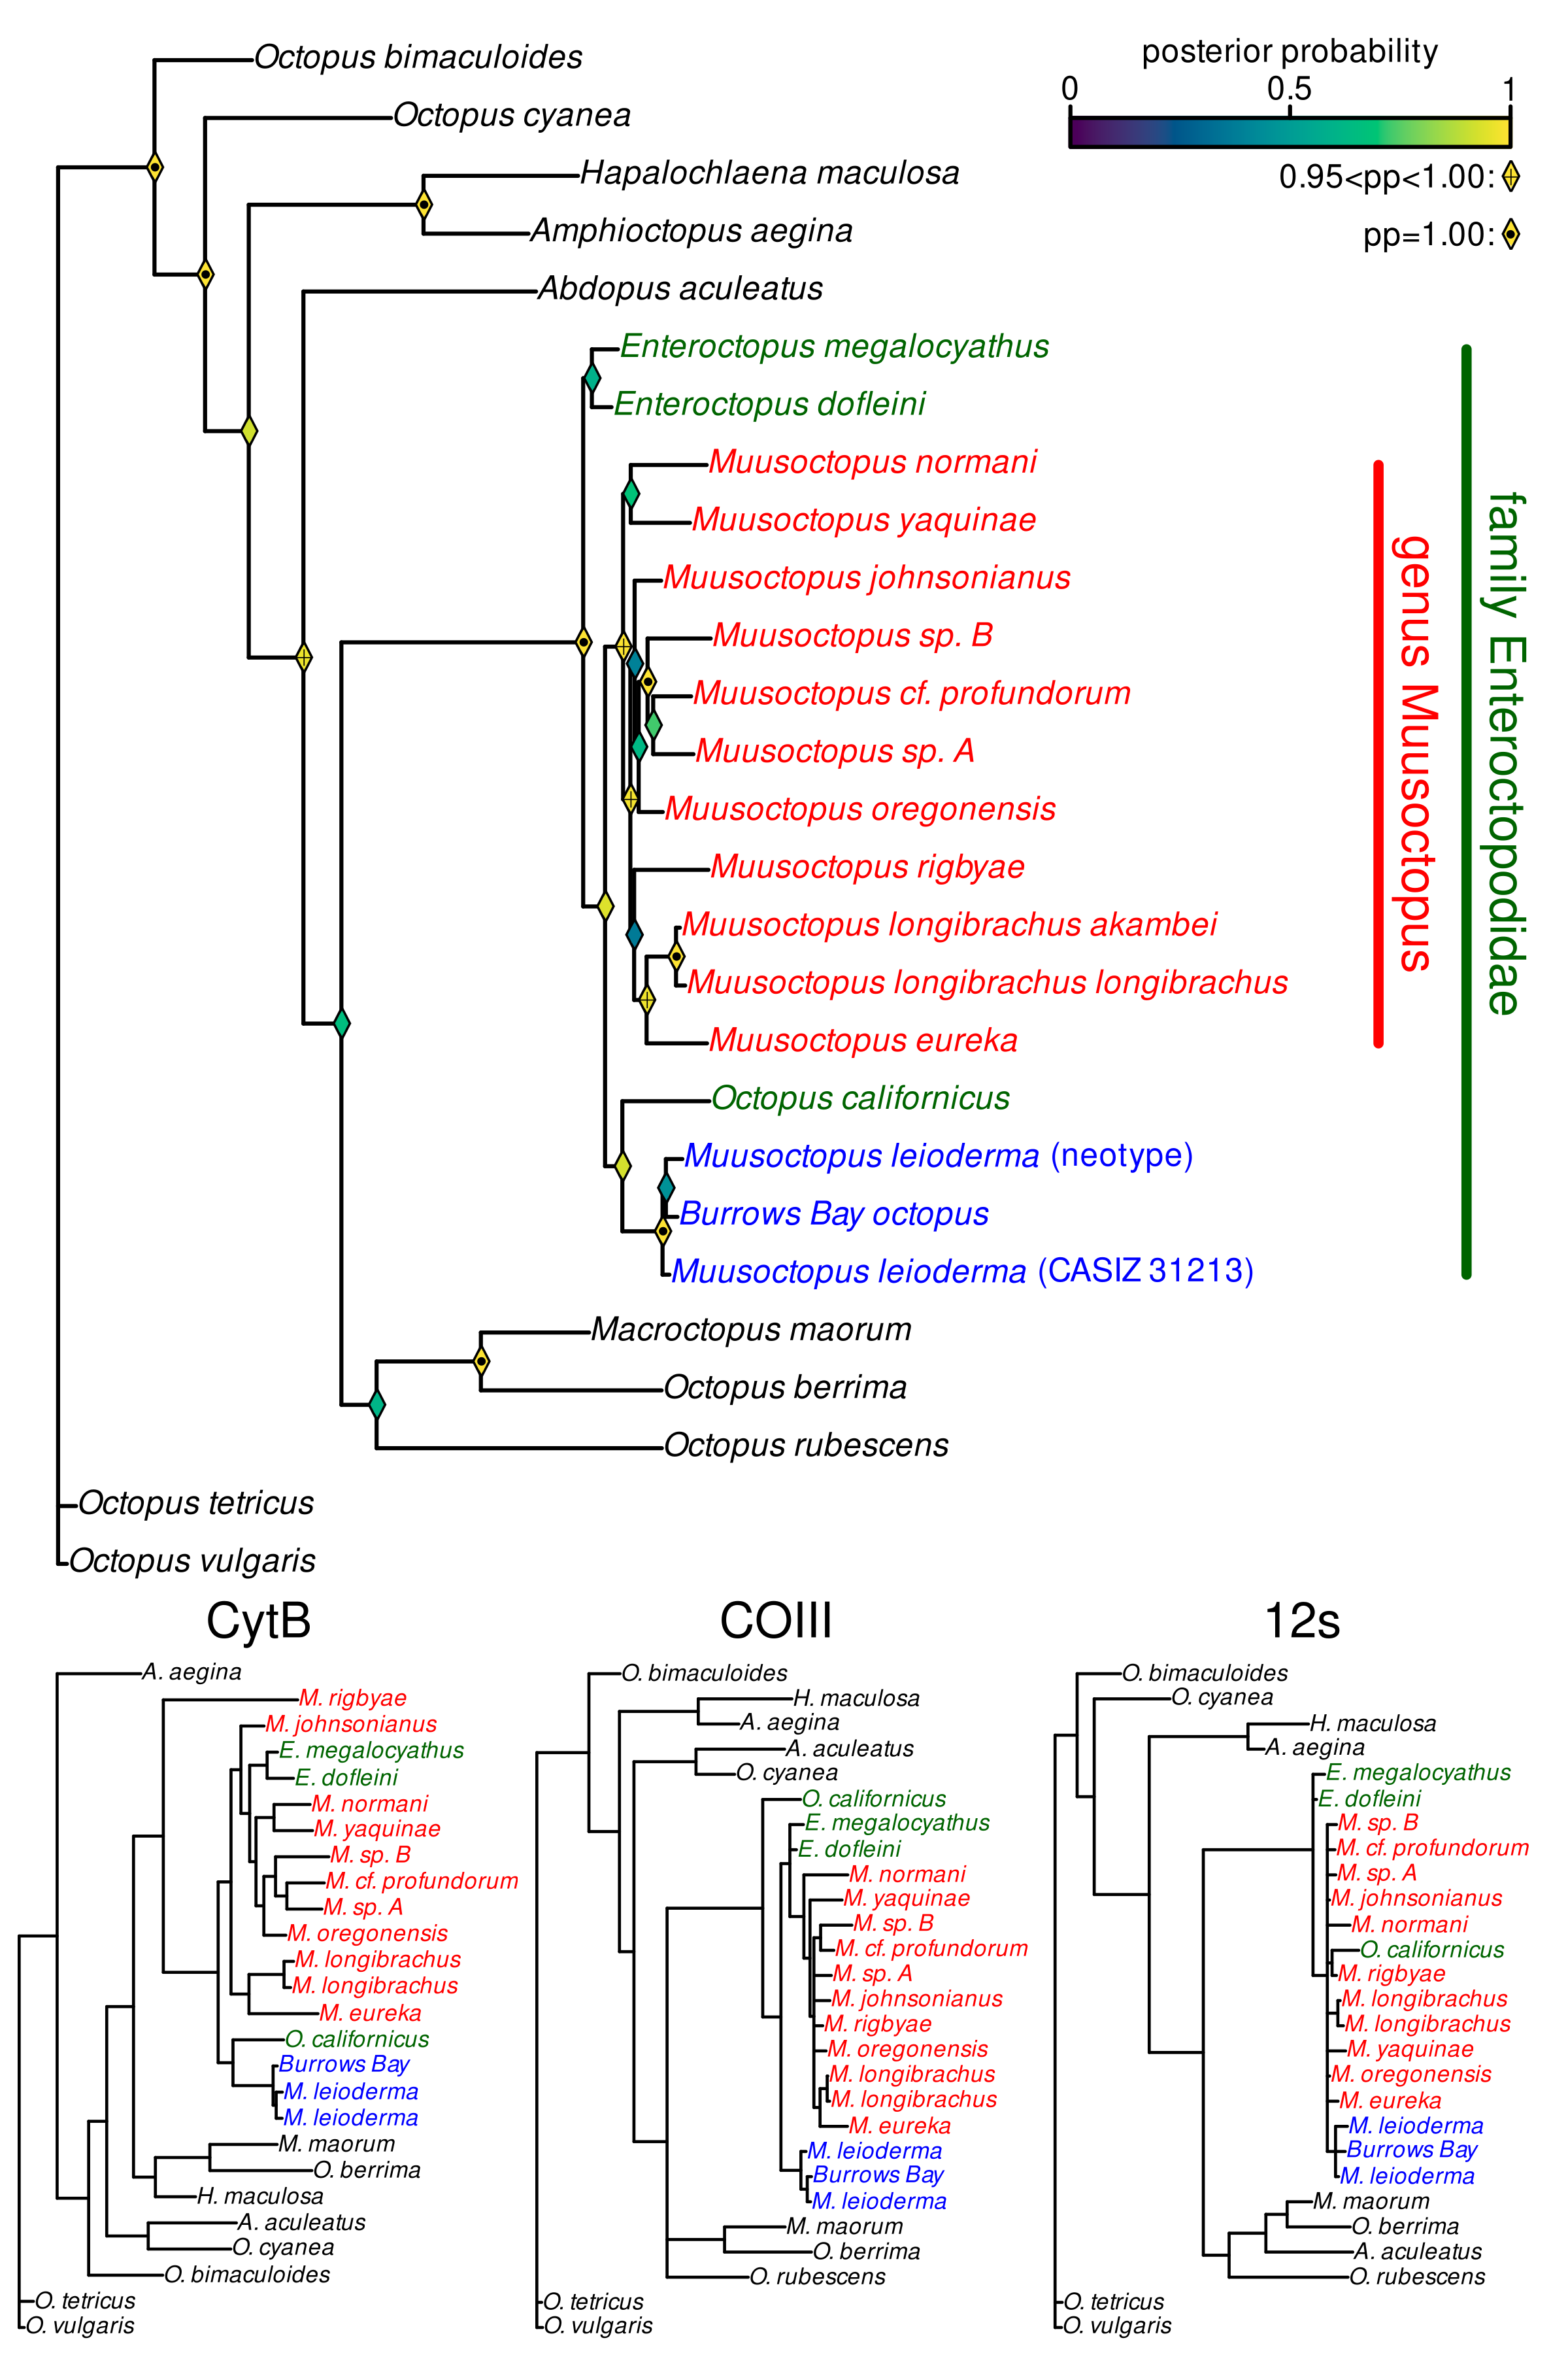
\includegraphics{Figure2.png}
\caption{Phylogeny of family Enteroctopodidae}
\end{figure}

\end{document}
